% !TEX program = xelatex
% Generated by make_tex.py from report.md.  Compile with XeLaTeX (or LuaLaTeX), twice:  xelatex report.tex
% Fonts: Latin Modern (text, math, code) and TeX Gyre Heros (headings); both ship with TeX Live.
\documentclass[paper=a4,fontsize=11pt,DIV=11,parskip=half,headings=small,numbers=noendperiod]{scrartcl}

\usepackage{amsmath,mathtools}
\usepackage{fontspec}
\usepackage{unicode-math}
\setmainfont{Latin Modern Roman}
\setsansfont{TeX Gyre Heros}[Scale=MatchLowercase]
\setmonofont{Latin Modern Mono}[Scale=0.94,HyphenChar=None]
\setmathfont{Latin Modern Math}
\usepackage{microtype}
\frenchspacing
\emergencystretch=2em

\usepackage{xcolor}
\definecolor{accent}{HTML}{1F4E79}
\definecolor{newcol}{HTML}{1B7F4B}
\definecolor{updcol}{HTML}{B45309}
\definecolor{findbg}{HTML}{EFF4FA}
\definecolor{limbg}{HTML}{FBF4E6}
\definecolor{limcol}{HTML}{C58B2A}
\definecolor{frontbg}{HTML}{F3F3F1}
\definecolor{rulegray}{HTML}{7A7A7A}

\usepackage{graphicx}
\graphicspath{{./}{figures/}}
\usepackage{booktabs,array,longtable,multirow}
\usepackage{enumitem}
\usepackage{needspace}
\usepackage{caption}
\usepackage{tcolorbox}
\tcbuselibrary{skins,breakable}

\usepackage[headsepline,footsepline=false,plainheadsepline=false]{scrlayer-scrpage}
\clearpairofpagestyles
\ihead{\sffamily\small Two trained models and a training experiment}
\ohead{\sffamily\small Version 11 \textperiodcentered{} 28 November 2026}
\cfoot*{\sffamily\small\pagemark}

\setkomafont{disposition}{\sffamily\bfseries\color{accent}}
\addtokomafont{section}{\Large}
\addtokomafont{subsection}{\large}
\setcounter{tocdepth}{2}
\setcounter{secnumdepth}{2}

\captionsetup{font=small,labelfont={sf,bf},labelsep=period,justification=raggedright,singlelinecheck=false,skip=6pt}

\setlist{itemsep=0.28em,topsep=0.3em,parsep=0pt,partopsep=0pt}
\setlist[itemize,1]{leftmargin=1.4em,label={\color{accent}\textbullet}}
\setlist[itemize,2]{leftmargin=1.3em,label={\color{accent}\textendash},itemsep=0.15em}
\setlist[enumerate,1]{leftmargin=2.0em,label={\color{accent}\sffamily\bfseries\small\arabic*.},itemsep=0.45em}

\renewcommand{\arraystretch}{1.16}
\setlength{\LTpre}{4pt}
\setlength{\LTpost}{8pt}
\renewcommand{\topfraction}{0.85}
\renewcommand{\bottomfraction}{0.7}
\renewcommand{\textfraction}{0.12}
\renewcommand{\floatpagefraction}{0.75}
\setcounter{topnumber}{2}
\setlength{\tabcolsep}{5pt}
\setlength{\heavyrulewidth}{0.9pt}
\setlength{\lightrulewidth}{0.5pt}

% text macros (robust, so they may appear in headings, captions and tables)
\DeclareRobustCommand{\lead}[1]{\textsf{\bfseries\color{accent}#1}}
\DeclareRobustCommand{\code}[1]{{\fontseries{m}\ttfamily #1}}
\DeclareRobustCommand{\hdr}[1]{\textsf{\bfseries #1}}
\DeclareRobustCommand{\boxlabel}[2]{{\sffamily\bfseries\small\color{#1}#2}}

% [NEW] and [UPDATED] tags
\newcommand{\tagpill}[2]{\tcbox[on line,colback=#1,colframe=#1,boxrule=0pt,arc=1.6pt,left=2.4pt,right=2.4pt,top=0.9pt,bottom=0.9pt,boxsep=0pt,tcbox raise base,fontupper={\sffamily\bfseries\fontsize{6.8}{7}\selectfont\color{white}}]{#2}}
\DeclareRobustCommand{\tagnew}{\texorpdfstring{\tagpill{newcol}{NEW}}{[NEW]}}
\DeclareRobustCommand{\tagupd}{\texorpdfstring{\tagpill{updcol}{UPDATED}}{[UPDATED]}}

% boxes: findings (blue), limits and caveats (amber), front matter (grey)
\newtcolorbox{findbox}[1]{enhanced,breakable,colback=findbg,colframe=findbg,boxrule=0pt,sharp corners,
  borderline west={2.4pt}{0pt}{accent},left=9pt,right=8pt,top=5pt,bottom=4pt,before skip=8pt,after skip=8pt,
  before upper={\boxlabel{accent}{#1}\par\nopagebreak\vspace{1pt}}}
\newtcolorbox{limbox}[1]{enhanced,breakable,colback=limbg,colframe=limbg,boxrule=0pt,sharp corners,
  borderline west={2.4pt}{0pt}{limcol},left=9pt,right=8pt,top=5pt,bottom=4pt,before skip=8pt,after skip=8pt,
  before upper={\boxlabel{limcol}{#1}\par\nopagebreak\vspace{1pt}}}
\newtcolorbox{frontbox}{enhanced,breakable,colback=frontbg,colframe=frontbg,boxrule=0pt,arc=3pt,
  left=10pt,right=10pt,top=6pt,bottom=6pt,before skip=10pt,after skip=10pt}

\usepackage[colorlinks=true,linkcolor=accent,urlcolor=accent,citecolor=accent,bookmarksnumbered=true,
  pdftitle={Tests on two trained models, and a training experiment on four more: torn-bigger-13 and elem-partitioned-long-boosted-1},pdfsubject={Version 11}]{hyperref}

\begin{document}

\begin{flushleft}
{\sffamily\bfseries\color{accent}\small\MakeUppercase{Version 11}\hspace{0.7em}\textcolor{rulegray}{\textperiodcentered}\hspace{0.7em}\textcolor{rulegray}{28 November 2026}\par}
\vspace{8pt}
{\sffamily\bfseries\fontsize{24}{28}\selectfont Tests on two trained models,\par}
\vspace{0pt}
{\sffamily\bfseries\fontsize{24}{28}\selectfont and a training experiment on four more\par}
\vspace{8pt}
{\ttfamily\fontsize{15}{19}\selectfont torn-bigger-13}\hspace{0.5em}{\sffamily\large (general transpositions, $S_{25}$)\par}
\vspace{3pt}
{\ttfamily\fontsize{15}{19}\selectfont elem-partitioned-long-boosted-1}\hspace{0.5em}{\sffamily\large (elementary transpositions)\par}
\vspace{6pt}
{\sffamily\color{rulegray}The algorithm, and a notion of density\par}
\vspace{6pt}
{\color{accent}\rule{\linewidth}{1.1pt}}
\end{flushleft}

Run on 2026-11-25 to 2026-11-27. \S\,\ref{sec:3.1}–\ref{sec:3.13} use the two trained checkpoints as they are,
with no retraining; \S\,\ref{sec:3.14}–\ref{sec:3.16} use four models that I trained on Spartan from your
\code{hpc-\allowbreak{}experiment} code (\S\,\ref{sec:6.1}). Section~\ref{sec:2.3} also uses one real training
file and the real test file. Code, raw results and the figures are in this folder; commands to reproduce are in
\S\,\ref{sec:7}.

\begin{frontbox}
\lead{Version history.}

\begin{enumerate}
\item Version 1: baseline, stratified accuracy, planted-chase tests and Gram spectrum (\S\,\ref{sec:2},
  \S\,\ref{sec:3.1}–\ref{sec:3.5}).
\item Version 2: layer-wise probes, irrelevance interventions and the elementary-transposition model
  (\S\,\ref{sec:3.6}–\ref{sec:3.8}).
\item Version 3: which model produced Figure 5b, and where its blocks are (\S\,\ref{sec:3.8}).
\item Version 4: the position-embedding ablation, Test 6b (\S\,\ref{sec:3.8}).
\item Version 5: probes and activation patching at the word positions (\S\,\ref{sec:3.9}, \S\,\ref{sec:3.10}),
  and the design of the training experiment for the Spartan cluster (\S\,\ref{sec:6.1}; code and README in
  \code{../\allowbreak{}hpc-\allowbreak{}experiment/}).
\item Version 6: the same probes and patching on the elementary model (\S\,\ref{sec:3.11}).
\item Version 7: attention patterns and single-head ablation of both models (\S\,\ref{sec:3.12}); the training
  experiment is now one single-GPU job per model (\S\,\ref{sec:6.1}).
\item Version 8: the results of the training run on Spartan (\S\,\ref{sec:3.14}–\ref{sec:3.16}), two more
  inference tests on the original models (\S\,\ref{sec:3.13}), and the block question for the elementary arm
  (\S\,\ref{sec:3.15}). The title changed accordingly.
\item Version 9: a correction to how the data seen by the original and by the retrained models is compared
  (\S\,\ref{sec:3.14}, \S\,\ref{sec:3.15}, \S\,\ref{sec:5} item 12). No new experiments.
\item Version 10: memorisation in \code{torn-\allowbreak{}bigger-\allowbreak{}13} and hops against points
  (\S\,\ref{sec:3.17}); the other runs in the Spartan model folder, with the block boundary in other seeds
  (\S\,\ref{sec:3.18}); a reassessment of several conclusions of versions 8 and 9 (\S\,\ref{sec:1},
  \S\,\ref{sec:3.14}, \S\,\ref{sec:3.16}, \S\,\ref{sec:4}, \S\,\ref{sec:5} item 13).
\item Version 11 (this one): the algorithm I think the general model learned (\S\,\ref{sec:4.1}) and the notion
  of density the results support (\S\,\ref{sec:4.2}).
\end{enumerate}

\lead{What is new in this version (version 11).} The markers \textbf{\tagnew{}} and \textbf{\tagupd{}} show only
what changed since version 10. Text without a marker is unchanged from version 10. Each new version clears the
previous version’s markers.

\begin{itemize}
\item \lead{\S\,\ref{sec:4.1} \tagnew{}:} what algorithm I think the general model learned: suffix composition
  at the word positions with a reach that grows about like pointer jumping, read by the query in the last block;
  its limit is the reach, and long training chains are memorised beside it.
\item \lead{\S\,\ref{sec:4.2} \tagnew{}:} the notion of density I think the results support: coverage of chain
  patterns modulo relabelling (which explains the paper’s $S_{10}\to S_{25}$ result), and the closure the
  training procedure adds to it (which decides the long-chain edge).
\item \lead{\S\,\ref{sec:1} \tagupd{}:} new item 29.
\end{itemize}
\end{frontbox}

\tableofcontents

% ====================================================================================================
% 1 Summary [UPDATED]
% ====================================================================================================
\section{Summary \tagupd{}}\label{sec:1}
\begin{enumerate}
\item \lead{Baseline reproduced.} On the paper’s real test file the model gets 2,000/2,000 words right,
  free-running. On freshly generated words free-running accuracy was 3,000/3,000. Teacher-forced word accuracy
  was 19,999/20,000, with 499,999/500,000 positions correct.
\item \lead{Every test word is outside the training support.} The real training data touches at most 10 points
  (\S\,\ref{sec:2.3}). All 2,000 words of the real test file touch 17 to 25 points (mean 21.6), and my fresh
  words behave the same way.
\item \lead{But each individual chase in a natural test word is short.} In the real test file the longest chase
  made 9 hops and visited 9 distinct points. In my 20,000 fresh words, a chase visited at most 10 distinct
  points, and only 7 of 500,000 slots reached 10. So a test word is globally outside the support while each of
  its output slots is locally inside it. The paper-style accuracy therefore says nothing about slots with long
  chases.
\item \lead{Planted-chase (“ladder”) tests: accuracy is governed mainly by the number of hops $L$. The number of
  distinct points $s$ has a much smaller effect.}
\begin{itemize}
\item Accuracy is essentially perfect up to $L\approx 12$ and falls steeply after $L\approx 15$.
\item At fixed $s=12$: 100\% ($L=11$), 98.8\% ($L=14$), 78.5\% ($L=17$), 54.2\% ($L=20$).
\item At $L=20$ the model is at about 50–56\% whether the chase visits 4 points or 21 (1,000 words per cell in
  the fixed-hop sweep).
\end{itemize}
\item \lead{So the hypothesis I proposed earlier, that accuracy collapses once a chase visits more distinct
  points than the training support ($s\ge11$), is not supported.} Chases with 11–14 distinct points (10–13 hops)
  were 99.8–100\% correct. In the fixed-hop sweep (\S\,\ref{sec:3.3}), crossing from $s\le10$ to $s\ge11$ costs
  a small, measurable amount, about 2 points at $L=16$ and 4 points at $L=20$ (standard errors about 1),
  compared with 30–35 points for going from $L=16$ to $L=20$.
\item \lead{Unresolved: why hop count matters.} Either the 5-layer network cannot follow longer chains, or long
  chains are too rare in training, or both. The data is consistent with both (\S\,\ref{sec:3.3}). Tests 1, 2 and
  6a (\S\,\ref{sec:3.6}–\ref{sec:3.8}) narrow this but do not settle it, and the tests at the word positions
  (\S\,\ref{sec:3.9}–\ref{sec:3.10}, items 15 and 16) make a depth limit a serious candidate; see items 12, 15
  and 16. Item 18 adds that the elementary model, which follows 80 hops, shows the same word-position staircase.
  Item 19 adds that both models have heads that link hop letters and that these are needed more as chains get
  longer, without explaining how the elementary model composes 80 hops. Items 20, 21, 24 and 25 separate two
  questions that version 8 ran together. With long chains in the data, five blocks get 24 hops right, so the
  architecture can represent such chains. That does not show that the rule
  \code{torn-\allowbreak{}bigger-\allowbreak{}13} learned is not limited by its depth: its accuracy on fresh
  chains falls with the number of hops whatever the number of points visited (item 25), from about the reach of
  its probe staircase (item 15), while it is right on every long chain of its own training file (item 24).
\item \lead{Token embeddings are close to $S_{25}$-invariant} (\S\,\ref{sec:3.5}), but one of my earlier
  predictions about their spectrum failed.
\item \lead{The training support is $m=10$}, measured from the real training data (\S\,\ref{sec:2.3}). The
  checkpoint config’s \code{ACTUAL\_\allowbreak{}GROUP\_\allowbreak{}SIZE = 16} does not describe that data. In
  an earlier version of this report I wrongly took 16 from the config.
\item \lead{Layer-wise probes (\S\,\ref{sec:3.6}).} At the position that predicts $p_k$, the pointer’s location
  after $r$ hops is linearly decodable for the first few hops only. For $r=1$ a probe reaches 97–99\% at layer
  3, for $r=4$ about 60\% at layers 4–5, and for $8\le r\le L-2$ it is at most 13\% (chance 4\%) in every layer.
  That holds even for $L=8$ and $L=12$, where the model is 100\% correct. The answer itself appears only after
  the last block. So no linear probe reads a step-by-step record of the chain at the query position (a nonlinear
  one is not excluded), and there is no linearly readable staircase of one hop per layer. Composition at the
  input positions is probed in \S\,\ref{sec:3.9} (item 15).
\item \lead{Irrelevance interventions (\S\,\ref{sec:3.7}).} For $L\le 12$ and for natural words the prediction
  depends on the hop letters and on nothing else. Replacing every letter that cannot touch the pointer leaves
  the prediction unchanged in 98.1–100\% of 800 words per set, and replacing one hop letter changes it in about
  96\% (planted chases). At $L=16$ and $L=20$ the same replacements change 16\% and 45\% of predictions, almost
  all of them near-ties, and accuracy does not fall (87.1\% to 88.0\%, and 48.5\% to 50.4\%). At $L=20$,
  replacing a hop letter that is read last, i.e. one of the chain’s final hops, changes the prediction only
  about 60\% of the time, against 95–98\% for hop letters read first.
\item \lead{Elementary-transposition model (\S\,\ref{sec:3.8}).} My NumPy port reproduces the model: 31,996 of
  32,000 slots correct on the real test file (99.9875\%, teacher-forced) and 500/500 words free-running. At
  fixed width 8 (the pointer stays inside 8 adjacent positions) accuracy is 99.8–100\% from 12 up to 80 hops.
  There is no hop-count cliff, and its training data contains chases of up to 78 hops (about 0.1\% of slots have
  56 or more). Accuracy falls only when the chase spans more positions than any training chase did (width at
  least 12): 95.6\% at width 16 with 24 hops, 90.0\% at width 16 with 40 hops. On 3,000 fresh words, 7 of the 8
  errors are at width 11 or more, which holds 590 of the 48,000 slots.
\item \lead{What this does to item 6.} The elementary model has the same architecture family (5 blocks, 6 heads;
  my NumPy code loads both) and follows chases of 40–80 hops when its training data contains chases that long.
  The general-transposition model’s cliff at 15–20 hops sits where its own training data ends
  (\S\,\ref{sec:3.3}). That favoured “rare in training” over “five layers cannot do it”, but it was never a
  proof: the two tasks differ (\S\,\ref{sec:3.8}), and I have not trained the general model on longer chains.
  The word-position results (items 15 and 16) weaken that lean: chain continuations are built layer by layer,
  which is how a depth limit would look, so I now treat the two readings as open (\S\,\ref{sec:5} item 8). The
  elementary model has the same word-position staircase and follows 80 hops (item 18), so the staircase does not
  by itself separate the two readings. The head-level results (item 19) do not separate them either. The
  training run separates the architecture from the learned rule (items 20, 21, 24 and 25): five blocks can
  follow 24 hops, so the cliff is not a limit of what the architecture can represent; whether
  \code{torn-\allowbreak{}bigger-\allowbreak{}13} learned a rule limited by its depth is open, and items 24 and
  25 make that the most coherent reading I have. The end of the training chains is not the explanation either:
  the decline on fresh chains starts at 13 to 15 hops, where the training file holds hundreds to thousands of
  chains (item 24).
\item \lead{Figure 5b (\S\,\ref{sec:3.8}).} The saved picture in the original repo’s
  \code{embedding\_\allowbreak{}pictures/} matches the
  \code{elem-\allowbreak{}partitioned-\allowbreak{}long-\allowbreak{}boosted-\allowbreak{}1} checkpoint in this
  repo (correlation 0.9999), and you confirmed it is Figure 5b. Its word positions split into two blocks at
  position 72, and the 16 output positions form a third block at 120, so the block sides are about 72 and 48,
  not 45. The training data shows nothing special at 45 or at 72.
\item \lead{Position-embedding ablation, Test 6b (\S\,\ref{sec:3.8}).} Swapping entries of the
  position-embedding table of the elementary model makes its answers follow the rearranged word: in 92.6–93.6\%
  of the slots where the two answers differ (about 1,700–2,000 slots per segment swap), and 1\% or fewer follow
  neither. Swaps that cross the block boundary at 72 behave the same as swaps inside a block (92.6–92.9\%
  against 92.9–93.6\%), so I find no sign that the boundary does anything the model relies on. The model reads
  the order of the letters from these vectors.
\item \lead{At the word positions, the continuation of a chain becomes readable one layer at a time
  (\S\,\ref{sec:3.9}).} For a letter $(a,b)$ at word position $t$, the “continuation” of endpoint $a$ is where a
  pointer that leaves the letter at $a$ ends up after the remaining letters to the left. A linear probe trained
  on letters whose chain has $h$ hops still to go decodes it with the following accuracy (chance 4\%): at $h=1$,
  27\% at layer 1, 56\% at layer 2 and 72–77\% at layers 3–5; at $h=2$ to 4, 4–9\% up to layer 2, 33–47\% at
  layer 3, 60–66\% at layer 4; at $h=5$ to 8, 4–6\% up to layer 2, 7–11\% at layer 3, 40–47\% at layer 4,
  56–57\% at layer 5; at $h=9$ to 12, 3–5\% through layer 3, 10\% at layer 4, 64\% at layer 5; at $h=13$ to 24,
  4–5\% through layer 4 and 74\% at layer 5. The reach grows with depth, roughly 1, 1, 4, 8 and 13 or more hops
  at layers 1 to 5. That is the pattern a log-depth (“pointer-jumping”) composition would give, and it would cap
  five blocks near 16 hops. A probe does not show the algorithm, and the high-$h$ bins come from my planted
  words only (\S\,\ref{sec:3.9}). The elementary model shows the same staircase at its word positions and still
  follows 80 hops (item 18). A five-block model trained on long chains does 24 hops (item 20), and its probes do
  not follow this staircase (item 22).
\item \lead{Activation patching agrees (\S\,\ref{sec:3.10}).} Corrupt one hop letter of a planted chain ($L=8$,
  12 or 16, model right on the clean word) and patch clean activations into the corrupted run. For a middle or
  last hop, restoring the clean activations at \emph{all word positions} after block 4 brings back the clean
  answer in every word (1.00 to two decimals in all six conditions), although the query position’s own state was
  computed from the corrupted word: the late part of the chain reaches the answer through the word positions,
  read in the last block. For the first hop, restoration falls to 33–51\% when the patch is made after block 2
  and to 8–10\% after block 3: the query position has taken in the first hops by then (consistent with
  \S\,\ref{sec:3.6}). Patching only the letters to the \emph{right} of the corrupted one (read earlier in the
  chase) restores the answer for a middle hop from layer 3 on (30–38\% after block 3, 72–93\% after block 4) and
  for the last hop from layer 2 on (43–77\% after block 2, 97–100\% after block 3); patching only the letters to
  its \emph{left} (read later) restores nothing in any condition. So the corrupted letter’s influence travels
  towards the letters read before it, the direction in which continuations are built.
\item \lead{The training experiment (\S\,\ref{sec:6.1}) was run on Spartan; its results are in items 20 to 23
  (\S\,\ref{sec:3.14}–\ref{sec:3.16}).} It ran as one single-GPU job per model (\code{bash
  submit.\allowbreak{}sh}). The three general arms finished their 200,000 steps (205M fresh words each; 5.3, 5.5
  and 8.6 hours), and the elementary arm was stopped by its time limit at step 106,250 of 110,000 (109M words,
  9.6 hours). The code matched \code{transformer.\allowbreak{}py} to 1e-6 and the data generators matched your
  real training statistics (tested on CPU before the run). One seed per arm.
\item \lead{The elementary model shows the same word-position staircase, and follows 80 hops
  (\S\,\ref{sec:3.11}).} I ran the tests of \S\,\ref{sec:3.9} and \S\,\ref{sec:3.10} on
  \code{elem-\allowbreak{}partitioned-\allowbreak{}long-\allowbreak{}boosted-\allowbreak{}1}. On natural words,
  a probe for the continuation of a chain is clearly above its layer-0 baseline for $h=1$ at layer 1 (86\%
  against 56\%), $h\le2$ at layer 2, $h\le4$ at layer 3, $h\le8$ at layer 4 (50\% and 45\% at $h=5$–6 and 7–8,
  against 18\% and 15\%), and only partly up to 12 to 16 at layer 5: about 1, 2, 4, 8 and 12 hops at layers 1 to
  5, a doubling pattern like the general model’s (1, 1, 4, 8, 13 or more). Yet this model follows chains of 80
  hops with 99.8\% accuracy (item 11), so a per-position reach of about $2^\ell$ does not by itself cap the hop
  length, and the argument I drew from \S\,\ref{sec:3.9} for a depth limit in the general model is weaker
  (\S\,\ref{sec:5} item 9). Patching agrees with \S\,\ref{sec:3.10} where it can be compared: with a middle or
  last hop corrupted ($L=12$ to 80), restoring all word positions after block 4 brings back the clean answer in
  every word, and with the first hop corrupted the repair works through layer 3 (0.97–1.00) and fails after
  block 4, at every $L$. One difference: restoring only the letters read later also repairs a corrupted first or
  middle hop (0.84 and 0.68 after block 3, $L=40$), which restored nothing in the general model. The probe
  numbers above $h=16$ exist only in planted words and are confounded with position (\S\,\ref{sec:3.11},
  Limits).
\item \lead{Attention heads link neighbouring hop letters, more of them are needed as chains get longer, and the
  elementary model’s reach doubles with depth (\S\,\ref{sec:3.12}).} I looked at the attention patterns of both
  models on planted chains and ablated one head at a time. (a) Both models have heads in blocks 1 to 3 whose
  attention goes to the next or the previous letter on the chain (up to 59\% of a letter’s attention, against
  4\% under uniform attention in the general model). A control on natural words shows this is content and not
  only position: the best of these heads give the next hop letter 3 to 4 times the attention of a non-chain
  letter at the same distance in the general model, and 13 to 40 times in the elementary model. (b) In the
  elementary model the hop offsets that heads attend to grow with depth: $\pm1$ in blocks 1 and 2, $\pm2$ and
  $\pm4$ in block 3, and from $\pm6$ to about $\pm12$ in block 4, on even offsets only; this matches the probe
  staircase of item 18. The general model shows $\pm1$ through block 3 and $+2$ and $+4$ in one head, so the
  doubling is less clear there. (c) Zeroing one head at the word positions costs more than 10 points for 1, 6
  and 12 of the 24 heads in blocks 1 to 4 at $L=8$, 12 and 16 (general model) and 8, 10 and 11 at $L=12$, 40 and
  80 (elementary model); the deepest heads of the elementary model matter only for long chains (block 4 head 1:
  1, 27 and 41 points lost at $L=12$, 40 and 80). (d) At the query position the heads read fixed ranges of word
  positions and pick chain letters within them (elementary model, $L=80$: block 4 head 0 reads the last 12
  letters, block 5 head 1 positions 72 to 83); I first read this as a rule about hop number, which was wrong
  (\S\,\ref{sec:5} item 10). (e) I did not find how 80 hops are composed: the largest offsets are about 10 to 12
  hops, and the probe cannot read the answer from the letters that block 5 reads. One head at a time cannot see
  redundancy, and attention is not causal.
\item \lead{Five blocks do 24 hops when the data contain such chains (\S\,\ref{sec:3.14}).} The model trained on
  half natural words and half planted chains of 3 to 25 hops (\code{g\_\allowbreak{}plant10}, whole words still
  on 10 points) gets 300 of 300 planted slots right in every cell I tested, for up to 24 hops and up to 25
  distinct points, which is outside the 10-point support; the same model with 8 blocks
  (\code{g\_\allowbreak{}plant10\_\allowbreak{}b8}) does the same. My prediction for the coverage reading (at
  least 90\% at 20 to 24 hops, including $s=14$ and 20) was met, but the control nearly met it too, because it
  has no cliff (item 21); so the planted arm’s advantage over the control is at 22 to 24 hops and for chains
  through few points only, and it says nothing about the original’s cliff. My prediction for the depth reading
  (the five-block planted model still falls off between 16 and 24 hops) failed: that refutes a limit of the
  architecture, not one of the rule the original learned (item 6). The 8-block arm says nothing about depth,
  because the five-block arm is already at the ceiling of the test (\S\,\ref{sec:5} item 11). Planted chains
  also bring the transition on natural words forward, by 1.7 times in steps with 5 blocks and 2.5 times with 8.
\item \lead{The control does not reproduce the original’s cliff, and both kinds of model follow chains beyond
  the ones they saw (\S\,\ref{sec:3.14}, \S\,\ref{sec:3.13}).} The control \code{g\_\allowbreak{}m10} has the
  original’s data distribution (natural words over 10 points) and gets 97–100\% at 14 to 20 hops (for 10 or more
  points), 95\% at 22 and 87\% at 24, where \code{torn-\allowbreak{}bigger-\allowbreak{}13} was at about 51\% at
  20 hops. Its weak spot is chains that stay on few points (65–74\% at 16 or more hops through 3 points), which
  natural words essentially never contain. The number of hops of a slot in a natural word is exactly
  Binomial(25, 0.18), so in its 205M words the control saw about 10 slots with 18 or more hops and, in
  expectation, none with 20 or more, yet it gets 97.7\% at 20. The elementary model does the same on its task:
  98.7\% at 100 hops and 92–95\% at 110 and 118, where my sample of its training data stops near 78 (Test 13).
  The original run differs from the control in several ways (205M distinct words, each seen once, against an
  8M-word file read 161 times; batch size; number of steps; schedule; seed), and I do not know which of them
  produced the original’s cliff.
\item \lead{A few word-position heads carry the chains in every general model, and the planted models differ
  from the original and the control in every internal measurement (\S\,\ref{sec:3.13}, \S\,\ref{sec:3.16}).} (a)
  In \code{torn-\allowbreak{}bigger-\allowbreak{}13} the four next-hop heads (b1h3, b2h5, b2h0, b3h4) zeroed
  together take the accuracy to 12\% at $L=8$ although each alone costs at most 3 points there (Test 14). (b)
  Greedy removal of word-position heads (Test 15): three of 24 heads bring the control to 18\% ($L=16$),
  \code{g\_\allowbreak{}plant10} to 31\% and \code{g\_\allowbreak{}plant10\_\allowbreak{}b8} (3 of 42) to 29\%
  ($L=24$); \code{e\_\allowbreak{}base} falls to 33\% with one head and to 25\% with eight ($L=80$), and 17 of
  its 24 heads cost more than 10 points singly. (c) In the planted models no single head’s word-dependent output
  is needed (mean replacement costs at most 6 points at $L=24$), the probes at the word positions read less
  (14–38\% at $h\ge5$, layer 5, for \code{g\_\allowbreak{}plant10}), and in the 8-block model the probe
  staircase and the hand-over of the first hop to the query are shifted three blocks later. (d) The attention of
  the general models stays at hop offsets $\pm1$ (one head at $+2$): no doubling, and I did not find the
  mechanism. (e) \code{e\_\allowbreak{}base} repeats the original elementary model’s staircase and doubling of
  attention offsets; its query takes in the first hop about one block earlier than the original’s. These are
  differences in measurements, with one seed per arm, linear probes trained within each arm and zero ablation,
  not a demonstrated difference in algorithm.
\item \lead{The block at position 72 has not formed in \code{e\_\allowbreak{}base} (\S\,\ref{sec:3.15}).} After
  109M words the pair of positions $(71,72)$ is as similar as an ordinary neighbour pair (cosine 0.26 against a
  median of 0.27); the original has its lowest value there (0.18 against 0.40). The position embeddings become
  smooth from the diagonal outwards from about step 4,000, before natural words reach 50\% (step 32,083), and
  are still smoothing at the end. The original elementary model saw 14 times as many words presented (96 epochs
  of 16M words), but \code{e\_\allowbreak{}base} saw about 7 times as many distinct words (109M against 16M).
\item \lead{\code{torn-\allowbreak{}bigger-\allowbreak{}13} is right on every long chain of its own training
  file, and not on fresh ones (\S\,\ref{sec:3.17}, Test 16).} On all its training slots with 14 to 18 hops
  (1,468 slots at 14, 270 at 15, 34 at 16, 4 at 17–18) it is at 100\%, while on fresh natural slots with the
  same number of hops it gets 0.976 at 14, 0.943 at 15, 0.868 at 16 and 0.72 at 17 (32 slots). Up to 12 hops
  training and fresh slots get the same margins. The decline therefore starts inside the range the file covers,
  and memorisation hides it on the training words. The fresh-data control is at 98–100\% on the same fresh
  slots, and \code{g\_\allowbreak{}plant10} at 100\% with a margin that does not depend on the number of hops.
\item \lead{The original’s limit is in hops, the control’s in points (\S\,\ref{sec:3.17}).} On planted chains
  through 5, 7 or 10 points \code{torn-\allowbreak{}bigger-\allowbreak{}13} gets nearly the same accuracy at
  every length (about 0.99 to 14 hops, 0.90 at 16, 0.7 at 18, 0.5 at 20 and 0.4 at 22), while the fresh-data
  control is at 0.95 at 22 hops through 10 points and fails only on chains that keep revisiting a few points
  (0.61 through 3 points).
\item \lead{The elementary models do not memorise their long chains (\S\,\ref{sec:3.17}).} In five elementary
  runs, training, validation and fresh slots with 40 to 80 or more hops get the same accuracy (99.3–100\%) and
  the same margins, although four of them end with a validation loss 40 to 3,000 times their training loss. So
  \code{torn-\allowbreak{}bigger-\allowbreak{}13}’s pattern is not a general effect of training on a static
  file, and a large gap between the logged losses is not by itself a sign of it.
\item \lead{This report is about the February 2025 \code{torn-\allowbreak{}bigger-\allowbreak{}13}, and the
  resume changed it little (\S\,\ref{sec:3.18}).} The repo checkpoint is the February model (161 epochs); the
  file now on Spartan was saved after a 24-epoch resume in November 2025 with a fresh optimiser. The resumed
  model is a little better at 15 to 22 hops (by 2 to 18 points, in every cell) and has the same shape of decline
  and the same memorisation.
\item \lead{The block boundary of Figure 5b appears in about half the runs with its config, at different places
  (\S\,\ref{sec:3.18}).} Of six fully trained runs with
  \code{elem-\allowbreak{}partitioned-\allowbreak{}long-\allowbreak{}boosted-\allowbreak{}1}’s config, three
  have a clear boundary (at 72, 81 and 78), one a weak one (about 79) and two none, unrelated to how long they
  trained (63 to 341 epochs); an older run has the sharpest boundary of all, at 69. In every model with a
  boundary several heads of the first block hardly attend across it, but chains that straddle it are followed as
  well as chains inside a block.
\item \lead{\tagnew{} The algorithm, and the notion of density (\S\,\ref{sec:4.1}, \S\,\ref{sec:4.2}).} I think
  \code{torn-\allowbreak{}bigger-\allowbreak{}13} composes, at each letter, where a pointer leaving it ends up
  after the rest of the word, with a reach that grows about like pointer jumping (1, 1, 4, 8, 13 or more hops
  after layers 1 to 5), and reads that at the chain’s first letter in the last block; its limit is the reach,
  and its long training chains are memorised beside it. The density notion that fits: the objects are slots
  through their chain patterns up to relabelling. Every test slot’s pattern is contained in the training
  patterns, which explains the paper’s result. Beyond that, containment is not enough: what the model
  generalises to depends on how often a pattern occurs and on the training procedure (\S\,\ref{sec:4.2}).
\end{enumerate}

% ====================================================================================================
% 2 Setup and provenance
% ====================================================================================================
\section{Setup and provenance}\label{sec:2}
\subsection{What was run}\label{sec:2.1}
\begin{itemize}
\item The model’s forward pass and greedy decoder were reimplemented in NumPy
  (\code{np\_\allowbreak{}transformer.\allowbreak{}py}), mirroring
  \code{scaling-\allowbreak{}generator/\allowbreak{}transformer.\allowbreak{}py}, including the attention
  scaling by $n_{\text{embed}}^{-1/2}$ and the mask (inputs attend bidirectionally; outputs attend to all inputs
  and causally to earlier outputs).
\item Weights come from \code{model.\allowbreak{}safetensors} (stored as bfloat16, upcast to float32).
\item Free-running decoding uses \code{force\_\allowbreak{}valid=\allowbreak{}True}, the repo’s own metric.
  Teacher-forced evaluation takes the argmax over the whole vocabulary at each output slot, given the true
  preceding outputs.
\end{itemize}

\subsection{Why I trust the reimplementation, and what is not checked}\label{sec:2.2}
\begin{itemize}
\item The mask I build equals the mask buffer stored in the checkpoint.
\item The cached incremental decoder agrees with a full forward pass to $1.7\times10^{-5}$ in the logits.
\item It scores 100\% on fresh words and 2,000/2,000 on the real test file. A faulty reimplementation would not.
\item \lead{Not done:} a direct comparison against the repo’s PyTorch code. PyTorch could not be installed in my
  sandbox (the package host was blocked).
\end{itemize}

\subsection{Test words and the training support}\label{sec:2.3}
\begin{itemize}
\item The test set is not in this repo (the real one is in \code{Midataur/\allowbreak{}permutations}, see
  below). For most tests I generated words to match
  \code{fast-\allowbreak{}data-\allowbreak{}gen/\allowbreak{}src/\allowbreak{}main.\allowbreak{}rs} for the
  general type: 25 letters, each an independent uniform draw from the $25^2=625$ tokens (token $=25a+b$), with
  the permutation computed by swapping positions as in \code{get\_\allowbreak{}permutation}.
\item \lead{Training support (measured).} The data is not in the latest commit of this repo. It is in
  \code{scaling-\allowbreak{}generator/\allowbreak{}data/\allowbreak{}torn\_\allowbreak{}bigger/} at commit
  \code{5863de5} (“torn-bigger-13”) of \code{Midataur/\allowbreak{}permutations}: 20 training files of 400,000
  words each (8M words) plus a 2,000-word test file. I read one training file and the test file
  (\code{data\_\allowbreak{}stats.\allowbreak{}py}, output in \code{data\_\allowbreak{}stats.\allowbreak{}txt}).
\begin{itemize}
\item Training words touch 7 to 10 distinct points (mean 9.93; 93\% touch exactly 10) and never more than 10.
  Their permutations move at most 10 points. So $m=10$, as in the paper.
\item 10.0\% of training letters are identity tokens, against 4.1\% in the test file.
\item Test words touch 17 to 25 points (mean 21.6).
\item The stored permutations equal the ones I recompute from the words, in both files, so my reading of the
  token convention is right.
\item
  \code{trained-\allowbreak{}models/\allowbreak{}torn-\allowbreak{}bigger-\allowbreak{}13-\allowbreak{}config.\allowbreak{}py}
  sets \code{ACTUAL\_\allowbreak{}GROUP\_\allowbreak{}SIZE = 16}, which does not match this data. Earlier I
  switched to $m=16$ because you suggested trusting the config over the paper. That was wrong: the config value
  does not describe the data. I have not checked the other 19 training files, and I cannot prove the checkpoint
  was trained on exactly these files, but it scores 2,000/2,000 on this test file.
\end{itemize}
\end{itemize}

% ====================================================================================================
% 3 Results
% ====================================================================================================
\section{Results}\label{sec:3}
\subsection{The pointer-chase picture (used throughout)}\label{sec:3.1}
\emph{What a word means.} A word is a sequence of $N$ letters $t_1,\dots,t_N$ (written here left to right; the
data generator indexes them $0,\dots,N-1$). Each letter is a transposition $s_{a,b}$ of two points $a\ne b$
among $n$ points, or the identity (a letter with $a=b$, which does nothing). The generator starts from the
arrangement $[0,1,\dots,n-1]$ and applies the letters in order from the left end, each one swapping the entries
at positions $a$ and $b$. The model’s target for output slot $k$ is the entry $p_k$ of the final arrangement. I
checked this in the generator
(\code{fast-\allowbreak{}data-\allowbreak{}gen/\allowbreak{}src/\allowbreak{}main.\allowbreak{}rs},
\code{get\_\allowbreak{}permutation}) and in
\code{permdata.\allowbreak{}py::\allowbreak{}apply\_\allowbreak{}words}, which uses the same convention.

\emph{Why the chase runs right to left.} The last letter is the last change to the arrangement, so the entry
that ends in slot $k$ sat, just before that letter, at the place the last letter sends $k$ to: at $k$ itself if
the letter does not touch $k$, and at the other endpoint if it does. Repeating this for the second-to-last
letter, and so on, walks back through the word from the right end to the left end. The entry found in the
initial arrangement is $p_k$, because the initial arrangement is the identity. In formula,
\[ p_k = t_1\bigl(t_2(\cdots t_N(k))\bigr), \]
where each $t_j$ is read as the map that exchanges $a$ and $b$ and fixes every other point, and the innermost
map $t_N$ acts first.

\emph{The pointer.} So for each slot $k$ I place a “pointer” at $k$ and read the word from the right end. At
each letter $s_{a,b}$, if the pointer is at $a$ it moves to $b$, if it is at $b$ it moves to $a$, and otherwise
it stays. The point where it stops after the left-most letter is $p_k$. Two things follow at once:

\begin{itemize}
\item A letter that moves the pointer is a \textbf{hop} (a \emph{hop letter}); the other letters are irrelevant
  to this slot. Different slots have different hop letters, and one letter can be a hop for several slots.
\item Only the hop letters decide $p_k$. If the pointer makes $L$ hops it visits at most $L+1$ distinct points,
  so the answer is determined by $L$ letters and nothing else in the word.
\end{itemize}

\emph{Worked example.} Take $n=13$ and the six letters (left to right) $\{9,12\}$, $\{4,5\}$, $\{1,9\}$,
$\{2,8\}$, $\{7,1\}$, $\{3,7\}$, and slot $k=3$. Reading from the right: $\{3,7\}$ moves the pointer $3\to7$;
$\{7,1\}$ moves it $7\to1$; $\{2,8\}$ does not touch point 1, so nothing happens; $\{1,9\}$ moves it $1\to9$;
$\{4,5\}$ does nothing; $\{9,12\}$ moves it $9\to12$. So $p_3=12$, with $L=4$ hops and $s=5$ distinct points
($3,7,1,9,12$). As a check in the generator’s own terms, swapping left to right carries the entry 12 along the
same path backwards, $12\to9\to1\to7\to3$, and it ends in slot 3.

\emph{What I record.} For each slot I record $L$ (the number of hops) and $s$ (the number of distinct points
visited, including the start). When I number the hop letters $1,\dots,L$ (\S\,\ref{sec:3.10}), hop 1 is the one
the pointer meets first, the right-most. On every word I check that the pointer’s final position equals the true
$p_k$. The elementary model (\S\,\ref{sec:3.8}) uses letters that swap neighbouring points $i$ and $i-1$; the
order of application and the chase are the same.

\subsection{Stratified accuracy on natural words}\label{sec:3.2}
Source: \code{strat\_\allowbreak{}summary.\allowbreak{}txt} (20,000 words, 500,000 slots, teacher-forced).

{\small\nopagebreak[4]
\begin{longtable}{@{}l r r@{}}
\toprule
\hdr{distinct points $s$} & \hdr{slots} & \hdr{errors} \\
\midrule
\endfirsthead
\toprule
\hdr{distinct points $s$} & \hdr{slots} & \hdr{errors} \\
\midrule
\endhead
\bottomrule
\endlastfoot
1–2 & 214,573 & 0 \\
3 & 146,448 & 1 \\
4 & 88,534 & 0 \\
5 & 36,284 & 0 \\
6 & 11,104 & 0 \\
7 & 2,552 & 0 \\
8 & 425 & 0 \\
9 & 73 & 0 \\
10 & 7 & 0 \\
\end{longtable}}

\begin{itemize}
\item The single error is at a slot with 2 hops and 3 distinct points, which is an easy case. One error in
  500,000 is noise, and I draw no conclusion from it.
\item The 95\% interval for the rarest bin ($s=10$, 7 slots) is [0.65, 1.0], so it carries almost no
  information.
\item Free-running: 3,000/3,000 (95\% interval [0.9987, 1.0]).
\end{itemize}

\subsection{Ladder (planted-chase) tests}\label{sec:3.3}
\lead{Design.} For one output slot I force the chase to make exactly $L$ hops and visit exactly $s$ distinct
points. All other letters are random but avoid the pointer’s current position, so they cannot move it. Hop
letters sit at random word positions (“spread”) or in the last $L$ letters (“contig”). Series:

\begin{itemize}
\item \emph{Minimal ladders:} $L=s-1$ (every hop reaches a new point).
\item \emph{Control:} $L=20$ hops with $s=4,6,8,10$.
\item \emph{Fixed support:} $s=12$ with $L=14,17,20$ (plus $L=11$ from the ladder series).
\end{itemize}

\begin{figure}[htbp]\centering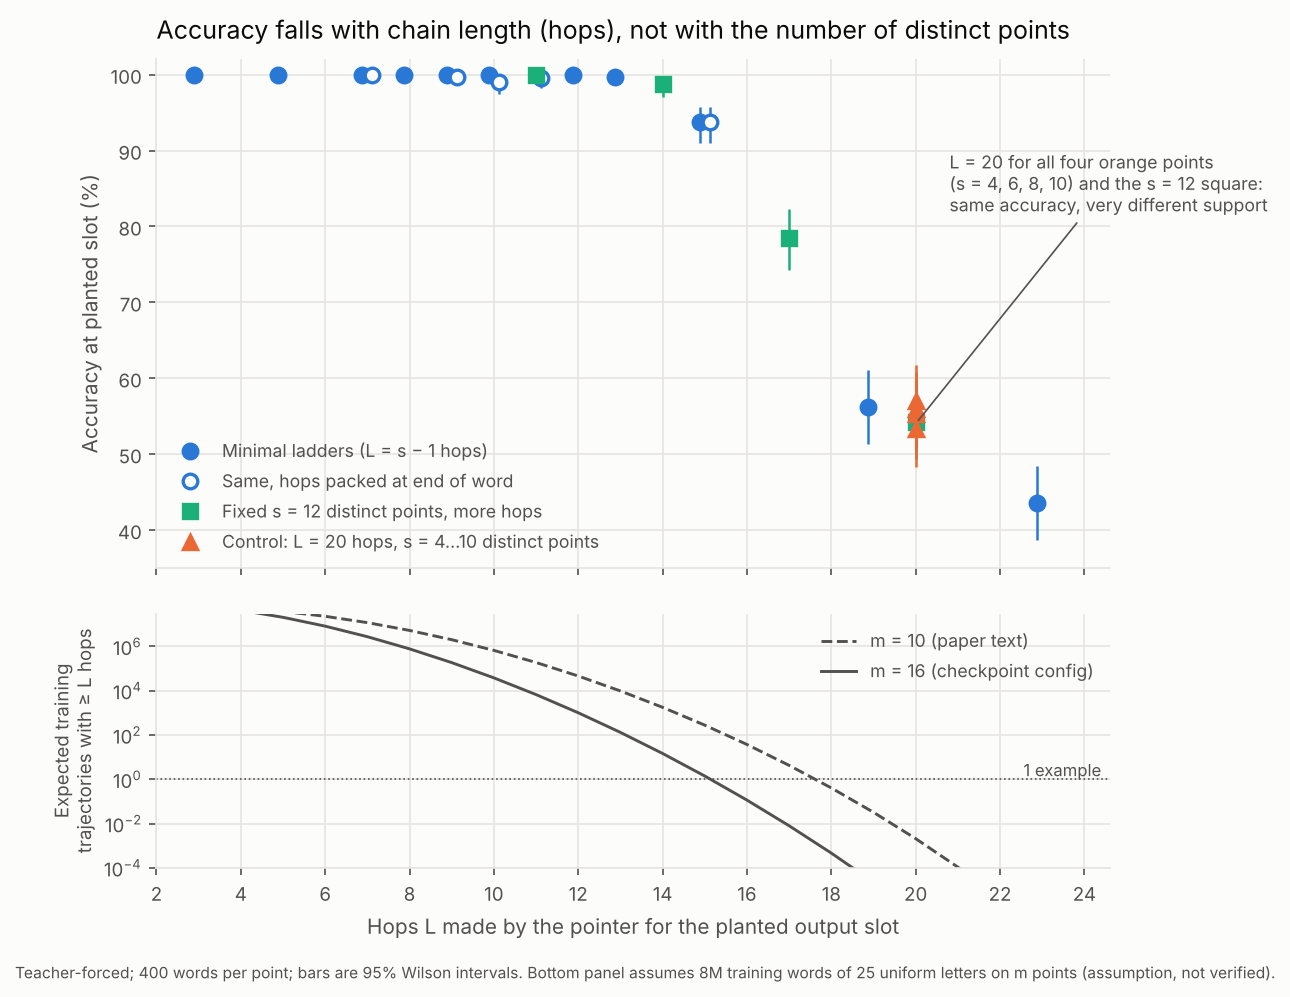
\includegraphics[width=0.88\linewidth]{fig_accuracy_vs_hops.png}\caption{Planted-chase accuracy against hop count $L$ (top), and the number of training slots with at least $L$ hops, from one real training file scaled to 8M words (bottom). Teacher-forced, 400 words per point, 95\% Wilson intervals.}\end{figure}

{\small\nopagebreak[4]
\begin{longtable}{@{}l r r r l r@{}}
\toprule
\hdr{series} & \hdr{$L$} & \hdr{$s$} & \hdr{free-running word} & \hdr{teacher-forced slot [95\% CI]} & \hdr{median logit margin} \\
\midrule
\endfirsthead
\toprule
\hdr{series} & \hdr{$L$} & \hdr{$s$} & \hdr{free-running word} & \hdr{teacher-forced slot [95\% CI]} & \hdr{median logit margin} \\
\midrule
\endhead
\bottomrule
\endlastfoot
ladder & 3 & 4 & 200/200 & 400/400 & 20.8 \\
ladder & 7 & 8 & 200/200 & 400/400 & 21.1 \\
ladder & 10 & 11 & 200/200 & 400/400 & 20.4 \\
ladder & 11 & 12 & 200/200 & 400/400 & 19.6 \\
ladder & 12 & 13 & 200/200 & 400/400 & 18.4 \\
ladder & 13 & 14 & 199/200 & 399/400 [98.6, 100] & 16.2 \\
ladder & 15 & 16 & 192/200 & 375/400 (93.8\%) [90.9, 95.7] & 10.2 \\
ladder & 19 & 20 & 116/200 & 225/400 (56.2\%) [51.4, 61.0] & 0.7 \\
ladder & 23 & 24 & 101/200 & 174/400 (43.5\%) [38.7, 48.4] & \ensuremath{-}0.4 \\
control & 20 & 4 & 96/200 & 221/400 (55.2\%) [50.4, 60.0] & 0.8 \\
control & 20 & 6 & 104/200 & 224/400 (56.0\%) [51.1, 60.8] & 1.8 \\
control & 20 & 8 & 118/200 & 228/400 (57.0\%) [52.1, 61.8] & 1.2 \\
control & 20 & 10 & 110/200 & 213/400 (53.2\%) [48.4, 58.1] & 0.5 \\
fixed $s=12$ & 14 & 12 & 197/200 & 395/400 (98.8\%) [97.1, 99.5] & 15.0 \\
fixed $s=12$ & 17 & 12 & 161/200 & 314/400 (78.5\%) [74.2, 82.2] & 5.0 \\
fixed $s=12$ & 20 & 12 & 119/200 & 217/400 (54.2\%) [49.4, 59.1] & 0.6 \\
contig & 11 & 12 & 198/200 & 398/400 (99.5\%) & 12.6 \\
contig & 15 & 16 & 198/200 & 375/400 (93.8\%) & 7.2 \\
\end{longtable}}

The full table (24 cells, including the remaining contig cells) is in
\code{ladder\_\allowbreak{}results.\allowbreak{}csv}.

\begin{findbox}{What it shows}
\begin{itemize}
\item At $L=20$ the accuracy is the same, within noise, for $s=4$ up to $s=12$ (400 words per cell). At $s=12$
  it varies from 100\% to 54\% as $L$ goes from 11 to 20. So $L$ is the dominant variable. The larger fixed-hop
  sweep below finds a small additional dependence on $s$ across the support boundary.
\item Where it fails, it fails softly: the median margin between the true logit and the best competitor goes
  from about 20 (easy) to about 0.6 at $L=20$. The model is close to indifferent rather than confidently wrong.
\item At $L\ge19$ accuracy is around 50\%, not near chance ($1/25$).
\item Hop letters packed at the end of the word give about the same accuracy as spread-out ones (e.g. both
  93.8\% at $L=15$).
\item Other output slots in the planted words stay at least 99\% correct in every cell.
\end{itemize}
\end{findbox}

\lead{Fixed-hop sweep across the support boundary.} The ladder cells confound $s$ and $L$, because a chase with
$s$ distinct points needs at least $s-1$ hops. To test the boundary directly I fixed $L$ and varied $s$ from
inside the training support ($s\le10$) to outside it ($s\ge11$). Script
\code{run\_\allowbreak{}beyond\_\allowbreak{}support.\allowbreak{}py}, teacher-forced, 1,000 words per cell,
seed 2027, result in \code{beyond\_\allowbreak{}support\_\allowbreak{}results.\allowbreak{}csv}.

{\small\nopagebreak[4]
\begin{longtable}{@{}r r l r@{}}
\toprule
\hdr{$L$} & \hdr{$s$} & \hdr{teacher-forced slot [95\% CI]} & \hdr{median logit margin} \\
\midrule
\endfirsthead
\toprule
\hdr{$L$} & \hdr{$s$} & \hdr{teacher-forced slot [95\% CI]} & \hdr{median logit margin} \\
\midrule
\endhead
\bottomrule
\endlastfoot
16 & 6 & 910/1000 (91.0\%) [89.1, 92.6] & 11.6 \\
16 & 9 & 895/1000 (89.5\%) [87.4, 91.3] & 9.9 \\
16 & 10 & 907/1000 (90.7\%) [88.7, 92.3] & 9.7 \\
16 & 11 & 896/1000 (89.6\%) [87.6, 91.3] & 9.3 \\
16 & 12 & 884/1000 (88.4\%) [86.3, 90.2] & 8.9 \\
16 & 17 & 876/1000 (87.6\%) [85.4, 89.5] & 6.2 \\
20 & 6 & 558/1000 (55.8\%) [52.7, 58.9] & 1.2 \\
20 & 9 & 529/1000 (52.9\%) [49.8, 56.0] & 0.5 \\
20 & 10 & 550/1000 (55.0\%) [51.9, 58.1] & 0.7 \\
20 & 11 & 508/1000 (50.8\%) [47.7, 53.9] & 0.2 \\
20 & 12 & 513/1000 (51.3\%) [48.2, 54.4] & 0.2 \\
20 & 17 & 499/1000 (49.9\%) [46.8, 53.0] & 0.0 \\
20 & 21 & 506/1000 (50.6\%) [47.5, 53.7] & 0.0 \\
\end{longtable}}

\begin{itemize}
\item Hop count dominates. Going from $L=16$ to $L=20$ costs about 30–35 points at every $s$ (for example 88.4\%
  to 51.3\% at $s=12$).
\item Pooling the cells inside the support ($s\le10$) and beyond it ($s\ge11$): at $L=16$ the accuracy is 90.4\%
  inside and 88.5\% beyond, a drop of 1.9 points (standard error 0.8). At $L=20$ it is 54.6\% and 50.6\%, a drop
  of 3.9 points (standard error 1.2).
\item So there is a small but detectable cost to leaving the support, about 2 to 4 points. It looks more like a
  small step at $s=10\to11$ than a smooth slope: the cells inside the support are flat (52.9–55.8\% at $L=20$)
  and so are those beyond it (49.9–51.3\%). With 1,000 words per cell I can’t rule out a gentle slope.
\item The cost of leaving the support is about a tenth of the cost of adding hops.
\item Caveat: at fixed $L$, larger $s$ also means a different word structure (fewer revisits of the same point),
  so this is not a pure change in support size.
\end{itemize}

\lead{Relation to training frequency (from the real training data).} I counted, in one of the 20 real training
files (400,000 words, \S\,\ref{sec:2.3}), the output slots whose pointer chase makes at least $L$ hops, and
scaled by 20 to the full 8M words. The tail is noisy because it rests on few observations.

\begin{center}\small
\begin{tabular}{@{}l r r r r r@{}}
\toprule
\hdr{$L \ge$} & \hdr{12} & \hdr{13} & \hdr{15} & \hdr{17} & \hdr{19} \\
\midrule
observed in file 1 & 2,310 & 483 & 18 & 1 & 0 \\
scaled to 8M words & 46,200 & 9,660 & 360 & 20 & 0 (upper 95\% bound about 60) \\
model accuracy at this $L$ & 100\% & 99.8\% & 93.8\% & 78.5\% & 56.2\% \\
\bottomrule
\end{tabular}
\end{center}

The accuracy cliff sits where the training data runs out of long chains: tens of thousands of slots with 12 or
more hops, a few hundred at 15, about 20 at 17, and none seen at 19 or more. At $L=17$ there are only about 20
examples in the whole training set and the model still gets 78.5\%. At $L=19$ to 20, where there are essentially
none, it still gets about 55\%. So it extrapolates partly beyond the chain lengths it saw, and degrades
gradually instead of failing at the edge of its training data. That fits “long chains are rare in training”. It
equally fits “five layers can only follow so many hops”, and this experiment cannot separate them. The numbers
come from one file of 20.

\begin{limbox}{Limitations of the design}
At $L=20$, 80\% of the word’s letters belong to one chain, so planted words differ from training words in other
ways too (\S\,\ref{sec:4}). The cells use 200 free-running and 400 teacher-forced words, so intervals are about
\ensuremath{\pm}5 percentage points. Teacher forcing lets the model see correct earlier outputs, which may help
it.
\end{limbox}

\subsection{Failure anatomy (exploratory, weak evidence)}\label{sec:3.4}
\code{run\_\allowbreak{}error\_\allowbreak{}anatomy.\allowbreak{}py} compares each wrong teacher-forced
prediction with the pointer’s positions after $0,1,\dots,L$ hops.

\begin{itemize}
\item For the minimal ladders this is uninformative: the chase path covers 20–24 of 25 points, so landing on it
  is nearly guaranteed.
\item For the few-point control ($s=4$) 71\% of failures land on the chase path (about 16\% expected by chance),
  which suggests failures are often intermediate states of the chase. But with only 4 points many hop counts map
  to the same point, which biases the “hops short of the end” measure downward.
\item For $s=12$, $L=20$: 79\% land on the path (about 46\% by chance), and the shortfall is spread widely
  (median 6 hops), not concentrated just short of the end.
\item So there is no clean “stops after $r$ hops” signature. I would not build on this.
\end{itemize}

\subsection{Gram spectrum of the token embeddings}\label{sec:3.5}
Tokens $s_{a,b}$ ($a<b$) are indexed by 2-element subsets of $\{1,\dots,25\}$, and $S_{25}$ acts on them. The
300-dimensional permutation module splits as
\[ M^{(23,2)}=S^{(25)}\oplus S^{(24,1)}\oplus S^{(23,2)},\qquad 300=1+24+275. \]
An $S_{25}$-invariant Gram matrix would be a combination of the three isotypic projectors (the Bose–Mesner
algebra of the Johnson scheme $J(25,2)$). \code{run\_\allowbreak{}gram.\allowbreak{}py} measures this, with a
null made by randomly relabelling the 300 tokens.

\begin{center}\small
\begin{tabular}{@{}>{\raggedright\arraybackslash}p{6.6cm} r r@{}}
\toprule
\hdr{quantity} & \hdr{trained} & \hdr{null (random relabelling)} \\
\midrule
fraction of Gram energy outside the three diagonal blocks & 0.0075 & 0.13 \\
off-diagonal energy not explained by the 3 class means & 0.021 & 1.00 \\
within-block relative eigenvalue spread (V0, V1, V2) & 0, 0.083, 1.01 & 0, 0.80, 2.64 \\
\bottomrule
\end{tabular}
\end{center}

\begin{itemize}
\item The embedding Gram is very close to invariant.
\item About 82\% of the symmetrised embedding energy lies in the additive part ($V_0\oplus V_1$, i.e. roughly
  $u_a+u_b$); regressing $E[s_{ab}]$ on $u_a+u_b$ gives $R^2=0.71$.
\item \lead{A prediction I made earlier did not hold cleanly:} I expected three eigenvalue clusters. $V_1$ is
  nearly one eigenvalue (28.8, spread 8\%), but the 275-dimensional block ($V_2$, mean eigenvalue 0.54) has a
  relative spread of about 1.0, so it does not collapse to a single value. It is tighter than the null but not
  clean.
\item $E[s_{ab}]$ and $E[s_{ba}]$ have cosine similarity about 0.74 (min 0.67). The paper described them as
  equal. They are related but not identical.
\item Only the general-transposition model was analysed.
\end{itemize}

\subsection{Layer-wise probes (Test 1)}\label{sec:3.6}
\lead{Question.} Does the model carry the pointer’s position after $r$ hops at the position that predicts $p_k$,
and in which layer does each one appear? If $x_r$ showed up at layer $\approx r$ and the staircase ran out near
$L\approx 15$, the five layers would be the bottleneck. If many hops showed up at once, the model would compose
in parallel and the cliff would need another explanation.

\lead{Design.} Planted chases with $L$ hops and $s$ distinct points, 4,000 words per design, designs
$(L,s)=(8,9),(12,13),(16,17),(20,21),(20,6)$. For each word I ran the model with teacher forcing and took the
residual-stream vector at position $25+k$ (the position whose output is $p_k$), after the embeddings (layer 0)
and after each of the five blocks (layers 1–5, before the final LayerNorm). Let $x_r$ be the pointer’s position
after $r$ hops, so $x_0=k$ and $x_L=p_k$. For every layer and every $r$ I fitted a ridge-regression probe from
the vector to the 25-way label $x_r$ on 60\% of the words, chose the ridge strength on 20\%, and report accuracy
on the remaining 20\% (800 words, standard error about 1.8 points at 50\%). Chance is 4\%. A control with
randomly shuffled training labels gave 3.7–4.6\% at layers 0 and 5 in every design
(\code{probe\_\allowbreak{}controls.\allowbreak{}json}). Script
\code{probe\_\allowbreak{}layers.\allowbreak{}py}.

\begin{figure}[htbp]\centering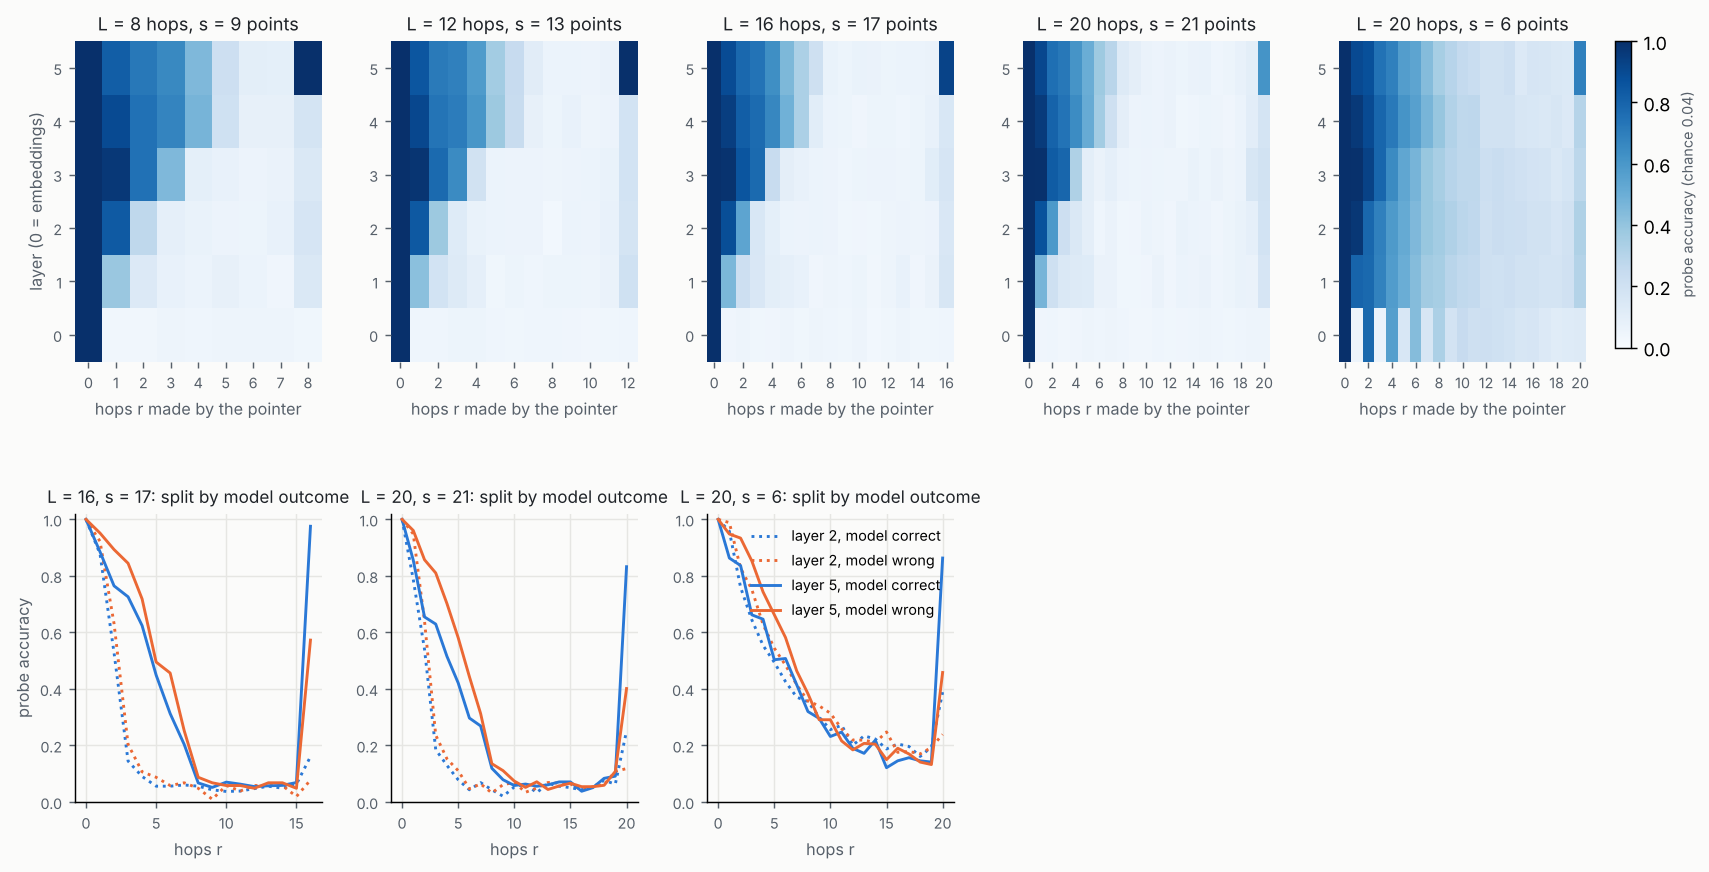
\includegraphics[width=1.00\linewidth]{fig_probe_layers.png}\caption{Probe accuracy for the pointer position after r hops, by layer, at the query position. Top: five designs (the colour scale is accuracy, chance 0.04). Bottom: for the designs where the model sometimes fails, probes at layers 2 and 5 split by whether the model got the slot right.}\end{figure}

Probe accuracy in percent, $L=12$, $s=13$ (the model is correct on all 800 test words here, so there is no split
by outcome):

{\small\nopagebreak[4]
\begin{longtable}{@{}l *{8}{r}@{}}
\toprule
\hdr{layer} & \hdr{$x_1$} & \hdr{$x_2$} & \hdr{$x_3$} & \hdr{$x_4$} & \hdr{$x_5$} & \hdr{$x_6$} & \hdr{$x_8$} & \hdr{$x_{12}$ (the answer)} \\
\midrule
\endfirsthead
\toprule
\hdr{layer} & \hdr{$x_1$} & \hdr{$x_2$} & \hdr{$x_3$} & \hdr{$x_4$} & \hdr{$x_5$} & \hdr{$x_6$} & \hdr{$x_8$} & \hdr{$x_{12}$ (the answer)} \\
\midrule
\endhead
\bottomrule
\endlastfoot
0 (embeddings) & 4 & 4 & 5 & 5 & 4 & 4 & 4 & 4 \\
1 & 42 & 18 & 13 & 9 & 4 & 5 & 5 & 20 \\
2 & 84 & 38 & 12 & 7 & 6 & 6 & 3 & 18 \\
3 & 98 & 78 & 65 & 19 & 6 & 6 & 5 & 18 \\
4 & 91 & 74 & 70 & 60 & 38 & 24 & 5 & 18 \\
5 & 85 & 71 & 69 & 58 & 36 & 24 & 6 & 100 \\
\end{longtable}}

\begin{findbox}{What it shows}
(the first four designs, which are minimal ladders: every $x_r$ is a different point).

\begin{itemize}
\item $x_0=k$ is decodable at 100\% in every layer. It is given by the query’s position, so it says nothing
  about mechanism.
\item \lead{Early hops appear in order, about one layer per hop.} $x_1$ is at 38–47\% after layer 1, 84–88\%
  after layer 2 and 97–99\% after layer 3. $x_2$ peaks at 75–86\%, $x_3$ at 67–79\% and $x_4$ at 47–66\%, each a
  layer or so later than the one before.
\item \lead{The staircase stops after about five hops.} $x_5$ and $x_6$ reach at most 51\% and 37\%, and $x_r$
  for $8\le r\le L-2$ stays at 3–13\% in every layer, for every design with $L\ge12$. (The state one hop before
  the answer, $x_{L-1}$, reaches 11\% at $L=16$ and 16\% at $L=20$ at layer 3, a little above chance.) At $L=8$,
  where the model is 100\% correct, $x_5,x_6,x_7$ are decodable at only 21\%, 10\% and 9\% in the last layer. So
  the model gets the right answer for 8 and 12 hops while the later intermediate positions are barely present at
  the query position.
\item \lead{The answer appears in the last block.} At layers 1–4 the probe for $x_L$ gives 14–20\%, which is
  above chance and which I do not explain. At layer 5 it gives 100\% for $L=8,12$, 92\% for $L=16$ and 61\% for
  $L=20$, close to the model’s own accuracy (100\%, 85.5\%, 48.6\% at the planted slot).
\item \lead{Correct versus wrong (bottom panels).} At layer 2 the probes behave almost identically on slots the
  model gets right and wrong. At layer 5 the wrong cases show higher, not lower, decodability for the early hops
  (for example $x_2$ at $L=16$: 89\% on wrong slots against 76\% on right ones). I have no explanation, and the
  split is exploratory.
\item \lead{The $(20,6)$ panel is not comparable.} With only 6 points, many $x_r$ coincide with $x_0$ (which is
  free) or with one another, so even the embeddings decode $x_2$ at 78\%. I would not read it.
\end{itemize}
\end{findbox}

\begin{findbox}{What this does and does not say}
\begin{itemize}
\item A purely sequential chase, one hop per layer with the state carried at the query position, cannot give
  correct answers for 8–12 hops with five blocks, and the probes agree: there is no sign of it past about 5
  hops. So “the staircase runs out around $L\approx15$” is not what happens. The first few hops are resolved in
  layers 1–4 and the rest is not visible.
\item \lead{How the model gets the later hops is not visible here.} Candidates are composition at the input-word
  positions (for example combining blocks of letters in parallel), a nonlinear encoding, or attention reading
  the letters directly. The probes cannot distinguish these.
\item Linear decodability is not use, and a failed probe does not prove absence.
\item Not done: probes at the input-word positions, and activation patching.
\end{itemize}
\end{findbox}

\subsection{Irrelevance interventions (Test 2)}\label{sec:3.7}
\lead{Question.} Does the model compute only along the chase, or do letters that cannot touch the pointer
influence the answer? If they do, failures at long $L$ could partly be distraction.

\lead{Design.} For an output slot $k$ a letter is \emph{irrelevant} if, at its turn in the right-to-left chase,
it does not contain the pointer’s current position (so it cannot change $p_k$). I replace irrelevant letters by
other letters that also avoid the pointer, so the true $p_k$ is unchanged by construction (checked on every
word), and ask whether the model’s prediction at slot $k$ changes. Conditions: all irrelevant letters replaced
(\code{full}), each with probability 1/2 (\code{half}), or all replaced by identity tokens (\code{identity}). As
a positive control, one random hop letter is replaced by an identity token, which changes the true $p_k$
(\code{delete1}). Word sets are planted chases with $L=8,12,16,20$ and natural random words (random slot), 800
each. The output prefix fed to the model is always the original word’s true outputs, so only the input letters
differ. Script \code{run\_\allowbreak{}irrelevance.\allowbreak{}py}.

Percentage of words whose prediction is unchanged (accuracy at the slot, before and after, for \code{full}):

\begin{center}\small
\begin{tabular}{@{}l c r r r r@{}}
\toprule
\hdr{word set} & \hdr{accuracy before \ensuremath{\to} after (\code{full})} & \hdr{\code{full}} & \hdr{\code{half}} & \hdr{\code{identity}} & \hdr{\code{delete1} (control)} \\
\midrule
planted $L=8$ & 100 \ensuremath{\to} 100 & 100.0 & 100.0 & 99.6 & 3.6 \\
planted $L=12$ & 100 \ensuremath{\to} 100 & 100.0 & 99.8 & 100.0 & 4.2 \\
planted $L=16$ & 87.1 \ensuremath{\to} 88.0 & 84.2 & 86.5 & 85.5 & 4.9 \\
planted $L=20$ & 48.5 \ensuremath{\to} 50.4 & 54.5 & 67.4 & 60.4 & 14.5 \\
natural words & 100 \ensuremath{\to} 100 & 100.0 & 100.0 & 98.1 & 14.6 \\
\bottomrule
\end{tabular}
\end{center}

The \code{delete1} figure for natural words, 14.6\%, is the share of slots with no hop at all (nothing to
delete), so it is not a failure of the control.

\lead{Confident versus near-tied predictions.} Splitting by the model’s baseline logit margin (confident: margin
above 5) shows where the changes at long $L$ come from:

\begin{center}\small
\begin{tabular}{@{}l r r@{}}
\toprule
\hdr{set} & \hdr{prediction unchanged, confident (n)} & \hdr{prediction unchanged, near-tied (n)} \\
\midrule
$L=16$, \code{full} & 96.4\% (501) & 63.9\% (299) \\
$L=20$, \code{full} & 99.0\% (104) & 47.8\% (696) \\
\bottomrule
\end{tabular}
\end{center}

\begin{figure}[htbp]\centering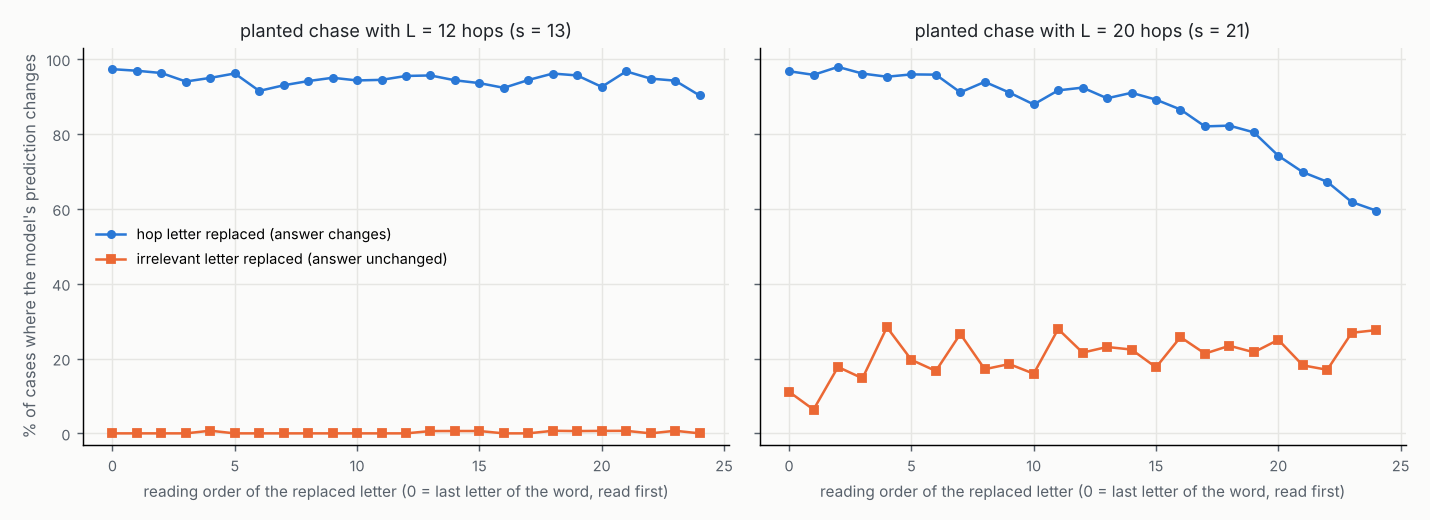
\includegraphics[width=1.00\linewidth]{fig_influence_map.png}\caption{Influence of single letters. Each point is the share of cases in which replacing one letter changes the model’s prediction, by the letter’s reading order. Blue: the letter is a hop letter (replaced by an identity token). Orange: the letter is irrelevant (replaced by a random pointer-avoiding letter). 300 words per panel.}\end{figure}

\begin{findbox}{What it shows}
\begin{itemize}
\item \lead{Locality holds at $L\le12$ and on natural words.} Replacing every irrelevant letter (13 to 23
  letters per word) leaves the prediction unchanged in 99.8–100\% of cases under \code{full} and \code{half},
  and in 98.1–100\% under \code{identity}. Every hop letter matters: replacing a single one changes the
  prediction in 94.6\% of the 3,600 hop letters tested at $L=12$ (0.2\% for irrelevant letters), with no strong
  dependence on where the letter sits in the word.
\item \lead{At $L=16$ and $L=20$ the predictions do move, but mostly where the model was undecided.} Confident
  predictions are 96–99\% stable, near-tied ones 48–64\%. Accuracy does not fall (87.1\% to 88.0\%, 48.5\% to
  50.4\%; with 800 words the standard error is about 1.2 to 1.8 points), so I see no systematic distraction. The
  changes look like a near-tie being re-rolled by any perturbation.
\item \lead{At $L=20$ the model partly ignores the chain’s last hops.} Replacing a hop letter that is read last
  (the first letters of the word) changes the prediction only about 60\% of the time, and the share rises
  steadily to 95–98\% for letters read first (right panel). Among the 104 confident $L=20$ words, replacing one
  random hop leaves the prediction unchanged in 34\%. This fits a model that sometimes stops following a long
  chain before the end. It does not prove that, and my earlier failure anatomy (\S\,\ref{sec:3.4}) found no
  clean “stops after $r$ hops” signature.
\end{itemize}
\end{findbox}

\begin{limbox}{Caveats}
Planted words at $L=16$ and $20$ are unlike training words anyway (\S\,\ref{sec:3.3}). Replacing irrelevant
letters with identity tokens makes natural words almost all identity, which is also unusual. Because the output
prefix is the \emph{original} one, other slots’ prefix tokens may disagree with the changed input. The model’s
output at slot $k$ ignored this at $L\le12$, which, if anything, strengthens the locality result.
\end{limbox}

\subsection{Elementary-transposition model (Tests 6a and 6b, and where Figure 5b comes from)}\label{sec:3.8}
\lead{The model.} \code{elem-\allowbreak{}partitioned-\allowbreak{}long-\allowbreak{}boosted-\allowbreak{}1}
(checkpoint in this repo; training and test data in \code{Midataur/\allowbreak{}permutations} at commit
\code{fdefb8c}). A word has 120 letters, each one of 16 tokens. Token $t\ge1$ swaps positions $t-1$ and $t$ and
token 0 is the identity, so the group is $S_{16}$ and the model emits 16 output slots. The vocabulary has 34
tokens (16 letter tokens, 16 output tokens, NULL, START) and the context is 136. The pointer chase is the same,
but every hop moves the pointer by $\pm1$. Instead of the number of distinct points I use the \textbf{width} $w$
of a chase: the number of adjacent positions it spans (largest minus smallest position visited, plus 1).

\lead{Port.} \code{np\_\allowbreak{}transformer.\allowbreak{}py} now takes \code{max\_\allowbreak{}group},
\code{input\_\allowbreak{}len} and \code{num\_\allowbreak{}trans}, and loads this model as
\code{NPTransformer(path, max\_\allowbreak{}group=\allowbreak{}16, input\_\allowbreak{}len=\allowbreak{}120,
num\_\allowbreak{}trans=\allowbreak{}16)}. The mask I build equals the stored one. As before I could not compare
with the repo’s PyTorch code; the check is the real test file below.

\lead{Real data} (first 100,000 rows of \code{train\_\allowbreak{}data1.\allowbreak{}csv}, i.e. 1.6M slots, and
the 2,000-word test file; \code{elem\_\allowbreak{}stats.\allowbreak{}py}, output
\code{elem\_\allowbreak{}stats.\allowbreak{}txt}).

\begin{itemize}
\item The stored permutations equal the ones I recompute (token $t$ swaps positions $t-1$ and $t$).
\item Training chases: hops per slot have mean 14.7, quantiles (5\%, 50\%, 95\%, 99\%, 99.9\%) of 0, 16, 38, 47,
  56, and a maximum of 78. Widths are at most 11 (no chase spans 12 or more positions); each training row uses
  at most 10 distinct tokens, from a window of up to 16.
\item Test file: hops mean 14.1 and maximum 29; width mean 5.6 and maximum 15; 0.53\% of slots have width 12 or
  more.
\item \lead{Model on the real test file:} 31,996 of 32,000 slots correct teacher-forced (99.9875\%), 1,996 of
  2,000 words, and 500 of 500 words free-running (first 500 test words). The four wrong slots (hops, width):
  (19, 14), (5, 4), (12, 13), (17, 13). Three of the four are at width 13 or more.
\end{itemize}

\lead{Planted cells} (\code{run\_\allowbreak{}elem\_\allowbreak{}cells.\allowbreak{}py}; 500 words per cell,
teacher-forced at the planted slot, seed 4242;
\code{elem\_\allowbreak{}cells\_\allowbreak{}results.\allowbreak{}csv}). The planted chase makes exactly $L$
hops and spans exactly $w$ positions; other letters avoid the pointer.

Teacher-forced accuracy at the planted slot (500 words per cell). Series A fixes the width at 8 and varies the
hops; series B and C fix the hops at 24 and 40 and vary the width.

\begin{center}\small
\begin{tabular}{@{}l *{5}{r}@{}}
\toprule
\hdr{A: width $w=8$, hops $L$} & \hdr{12} & \hdr{24} & \hdr{40} & \hdr{56} & \hdr{80} \\
\midrule
correct (of 500) & 500 & 500 & 500 & 500 & 499 \\
median logit margin & 22.9 & 22.8 & 21.9 & 20.6 & 16.7 \\
\bottomrule
\end{tabular}
\end{center}

\begin{center}\small
\begin{tabular}{@{}l *{6}{r}@{}}
\toprule
\hdr{B: $L=24$ hops, width $w$} & \hdr{4} & \hdr{8} & \hdr{11} & \hdr{12} & \hdr{14} & \hdr{16} \\
\midrule
correct (of 500) & 500 & 500 & 500 & 500 & 496 & 478 \\
median logit margin & 23.1 & 23.1 & 22.5 & 21.8 & 18.2 & 12.1 \\
\bottomrule
\end{tabular}
\end{center}

\begin{center}\small
\begin{tabular}{@{}l *{4}{r}@{}}
\toprule
\hdr{C: $L=40$ hops, width $w$} & \hdr{8} & \hdr{11} & \hdr{12} & \hdr{16} \\
\midrule
correct (of 500) & 500 & 500 & 499 & 450 \\
median logit margin & 21.4 & 20.0 & 18.9 & 10.4 \\
\bottomrule
\end{tabular}
\end{center}

95\% Wilson intervals: 500/500 is [99.2, 100]; 499/500 is [98.9, 100]; 496/500 (99.2\%) is [98.0, 99.7]; 478/500
(95.6\%) is [93.4, 97.1]; 450/500 (90.0\%) is [87.1, 92.3].

\begin{figure}[htbp]\centering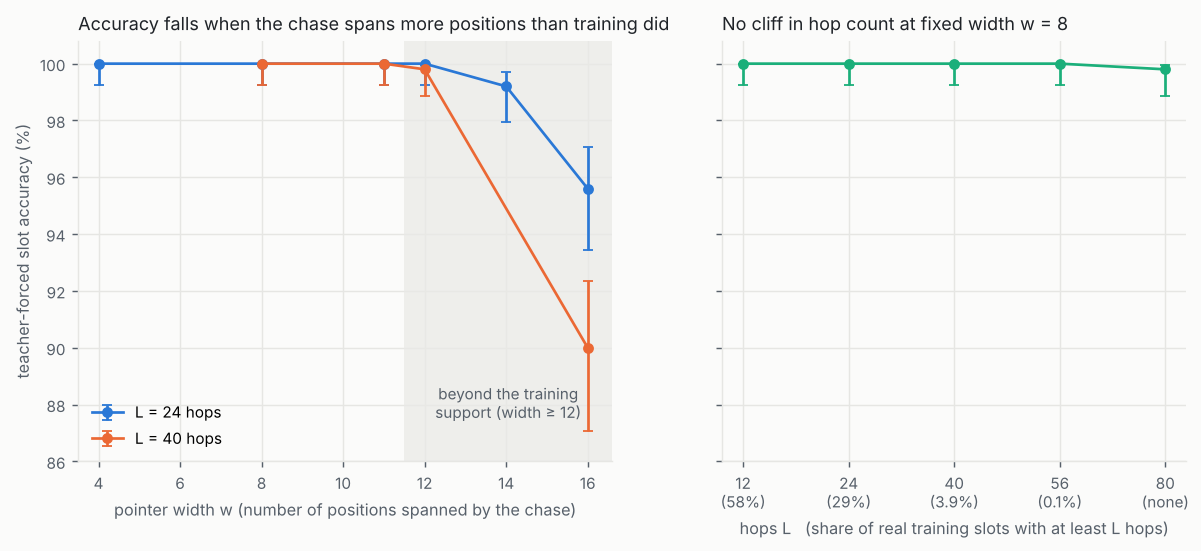
\includegraphics[width=1.00\linewidth]{fig_elem_cells.png}\caption{Elementary model, planted chases. Left: accuracy against width at 24 and 40 hops; the shaded region is wider than any training chase. Right: accuracy against hops at width 8, with the share of real training slots having at least that many hops under each tick. Teacher-forced, 500 words per point, 95\% Wilson intervals.}\end{figure}

\lead{Fresh natural words} (3,000 words, 48,000 slots; \code{elem\_\allowbreak{}natural.\allowbreak{}npz}). Slot
accuracy is 47,992/48,000 (99.983\%) and word accuracy 2,992/3,000 (99.73\%). By width:

\begin{center}\small
\begin{tabular}{@{}l r r@{}}
\toprule
\hdr{width} & \hdr{slots} & \hdr{errors} \\
\midrule
1–7 & 41,231 & 0 \\
8–10 & 6,179 & 1 \\
11 & 375 & 4 \\
12 or more & 215 & 3 \\
\bottomrule
\end{tabular}
\end{center}

By hop count the 8 errors are spread across the bins with 10–24 hops (3, 3 and 2 errors in bins of 21,300,
17,537 and 3,596 slots), and there are none among the 213 slots with 25 or more hops. I see no pattern with hop
count.

\begin{findbox}{What it shows}
\begin{itemize}
\item \lead{For this model, width is what matters, not hop count.} At width 8 accuracy is 99.8–100\% from 12 to
  80 hops. Training chases reach 78 hops, so $L=80$ is only just past the longest one seen and this is not an
  extrapolation test.
\item \lead{Leaving the trained width costs a few points, and more as chains get longer.} At width 16 (five
  beyond the training maximum of 11) accuracy is 95.6\% at 24 hops and 90.0\% at 40 hops. The margin falls
  smoothly (23 to 12 at $L=24$), so the failure is soft, as for the general model (\S\,\ref{sec:3.3}).
\item \lead{Degradation starts at the rare tail of the support, not exactly at its edge.} Width 11 is within the
  support but holds about 0.4\% of training slots, and it has 4 errors in 375 slots (1.1\%), against 1 error in
  47,410 slots at widths below 11.
\item \lead{Contrast with the general model.} There, accuracy fell steeply with hop count at fixed $s$
  (\S\,\ref{sec:3.3}) and depended only weakly on $s$. Here it is nearly flat in hop count and depends on width.
  The two training sets differ in the way that matters: the general model’s training data had essentially no
  chase of 19 or more hops, whereas the elementary model’s had many (3.9\% of slots with 40 or more).
\item \lead{Caveats on that comparison.} Hops of $\pm1$ inside a window of at most 11 positions are not the same
  computation as arbitrary jumps among 25 points, and many of the hops in a narrow window are back and forth.
  The width limit of the elementary model and the hop limit of the general model are both coverage effects of
  the training data, but I cannot show from this that the general model would behave like the elementary one if
  it were trained on long chains.
\end{itemize}
\end{findbox}

\lead{Which model produced Figure 5b (position-embedding self-similarity, $n=16$).} I searched the history of
\code{Midataur/\allowbreak{}permutations} for it (\code{fig5b\_\allowbreak{}provenance.\allowbreak{}py}, output
\code{fig5b\_\allowbreak{}provenance.\allowbreak{}txt}).

\begin{itemize}
\item \code{scaling-\allowbreak{}generator/\allowbreak{}mechanistic.\allowbreak{}ipynb} holds no PNG outputs at
  any commit; its plots are stored as plotly data, which still contains the matrices. The repo also contains
  four saved pictures in \code{scaling-\allowbreak{}generator/\allowbreak{}embedding\_\allowbreak{}pictures/}
  (token and position embeddings for \code{torn-\allowbreak{}bigger-\allowbreak{}13} and
  \code{elem-\allowbreak{}partitioned-\allowbreak{}long-\allowbreak{}boosted-\allowbreak{}1}), all added in
  commit \code{f262ca2} (2025-02-13).
\item Decoding each saved position picture back into similarity values and comparing with the cosine matrix of
  the position embeddings of the checkpoints in this repo gives correlation 0.9999 (elementary) and 1.0000
  (general), with a largest difference of 0.005, which is the colour quantisation. The 50\ensuremath{\times}50
  notebook plot of the general model matches its checkpoint exactly too.
\item \lead{You confirmed that the saved picture
  \code{position/\allowbreak{}elem-\allowbreak{}partitioned-\allowbreak{}long-\allowbreak{}boosted-\allowbreak{}1.\allowbreak{}png}
  is exactly Figure 5b.} So Figure 5b is the position-embedding similarity of the
  \code{elem-\allowbreak{}partitioned-\allowbreak{}long-\allowbreak{}boosted-\allowbreak{}1} checkpoint in this
  repo, 136 positions (120 word positions and 16 output positions). The saved 50\ensuremath{\times}50 picture
  for the general model matches \code{torn-\allowbreak{}bigger-\allowbreak{}13} in the same way; I expect it is
  the paper’s Figure 4b, but you have not confirmed that.
\item Three other 136\ensuremath{\times}136 pictures exist in the notebook history. Judged on off-diagonal
  structure, the ones at \code{fdefb8c} (2025-02-11) and \code{5863de5} (2025-02-12) have correlations 0.37 and
  0.80 with the final checkpoint, which suggests earlier training states of the same run, and the one at
  \code{1fb98be}/\code{dcb73d1} (2025-02-15/16) is unrelated to it (correlation 0.00).
\end{itemize}

\lead{Where its blocks are.} In the matrix of Figure 5b the word positions split at \textbf{72}: positions 0–71
and 72–119 form two blocks, with rows 72 and 73 transitional, and the 16 output positions 120–135 form a third.
The cosine between neighbouring positions dips at 71/72 (0.18, against about 0.4 elsewhere) and at 119/120
(0.06). The blocks of word positions therefore have sides about 72 and about 48 (46 or 47 if the transitional
rows are left out), not 45. I found no boundary of comparable sharpness elsewhere among the word positions. In
version 2 of this section I wrote that this checkpoint was not a clear example of the block and that I had no
seed that shows it. That was wrong: I looked for a boundary at 45, and the picture I made
(\code{elem\_\allowbreak{}pos\_\allowbreak{}gram.\allowbreak{}png}) used a colour scale that hid the structure.
This checkpoint is the example.

\lead{Position 45 in the training data} (\code{elem\_\allowbreak{}data\_\allowbreak{}stats.\allowbreak{}py},
\code{elem\_\allowbreak{}data\_\allowbreak{}stats.\allowbreak{}txt}, 400,000 training rows and the test file). I
found no structure at 45 or at 72. The training rows are position-stationary: for every position the token
histogram is consistent with the pooled one (chi-square $z$ scores between $-1.9$ and $+1.6$ over 120 positions,
none beyond 3; $z$ at positions 40–50 between $-0.9$ and $+1.5$), and the mean Coxeter length of the product of
the first $i$ letters is smooth through $i=45$ (second differences below 0.01). Training outputs move at most 13
points and have Coxeter length at most 42, while the test file reaches 16 points and length 48 (0.35\% of test
outputs have length 45 or more, against none in training). The test file’s token histogram is flat (0.062 each)
while training’s is bell-shaped (0.02 at the ends, 0.085 in the middle). I did not check position 72
specifically beyond the same stationarity test, which covers all 120 positions.

\lead{Test 6b: position-embedding ablation}
(\code{run\_\allowbreak{}pos\_\allowbreak{}ablation.\allowbreak{}py}, results in
\code{pos\_\allowbreak{}ablation\_\allowbreak{}results.\allowbreak{}json}). I edited the position-embedding
table of the elementary model in memory, so that the letter at word position $i$ is given the vector of position
$\sigma(i)$, and ran the real test words. If the model reads the order of the letters from the embeddings, its
answers should follow the \emph{rearranged} word $w'$, where $w'[\sigma(i)]=w[i]$. For each slot where the true
answer for $w$ and for $w'$ differ, I record whether the prediction equals the answer for $w$ (original), for
$w'$ (rearranged) or neither. The unedited model is 100\% correct on these words (150 words). Teacher forcing
with the original word’s true outputs as the prefix.

Segment swaps (two segments of 24 positions exchanged; 150 words):

{\small\nopagebreak[4]
\begin{longtable}{@{}>{\raggedright\arraybackslash}p{6.0cm} r r r r@{}}
\toprule
\hdr{swap} & \hdr{slots} & \hdr{original} & \hdr{rearranged} & \hdr{neither} \\
\midrule
\endfirsthead
\toprule
\hdr{swap} & \hdr{slots} & \hdr{original} & \hdr{rearranged} & \hdr{neither} \\
\midrule
\endhead
\bottomrule
\endlastfoot
inside block 1, adjacent: 0–23 with 24–47 & 1,723 & 6.2\% & 92.9\% & 1.0\% \\
inside block 1, far: 0–23 with 48–71 & 1,944 & 6.0\% & 93.3\% & 0.8\% \\
inside block 2: 72–95 with 96–119 & 1,751 & 5.7\% & 93.6\% & 0.7\% \\
across 72, adjacent: 48–71 with 72–95 & 1,766 & 6.2\% & 92.9\% & 0.8\% \\
across 72, far: 24–47 with 96–119 & 1,953 & 6.0\% & 92.6\% & 1.3\% \\
across 72, far: 0–23 with 96–119 & 2,024 & 5.9\% & 92.6\% & 1.5\% \\
\end{longtable}}

Single swaps of two neighbouring positions $(i,i+1)$ for every $i$ from 0 to 118 (150 words each, 5,832 slots
pooled): 93.6\% of the predictions follow the rearranged word. For the swap across the boundary, $(71,72)$, it
is 95\% (60 slots), which lies within the spread of the other pairs (the lowest is 85\%, at $i=35$, with 40–60
slots per pair).

\begin{itemize}
\item \lead{The model takes the order of the letters from the position vectors.} About 93\% of the answers
  follow the rearranged word, and 1\% or fewer follow neither, so the model is not broken by these edits, it is
  consistent with a reordered word.
\item \lead{Crossing 72 makes no measurable difference.} Segment swaps across the boundary (92.6–92.9\%) and
  inside a block (92.9–93.6\%) are alike, and so is the single swap at $(71,72)$. I find no sign that the model
  relies on the block boundary.
\item \lead{Not explained:} the 6–7\% of differing slots that keep the original answer. I have not looked into
  which slots they are.
\item \lead{Limits.} This shows whether the model uses the structure, not why training produced the blocks. Only
  swaps were tried: I did not remove the block structure itself (for example by projecting out the directions
  that separate the blocks), I did not test the 16 output positions, and the single-swap counts are small (40–60
  slots per pair). Teacher forcing may help the model.
\end{itemize}

\subsection{Probes at the word positions (Test 7)}\label{sec:3.9}
\begin{figure}[htbp]\centering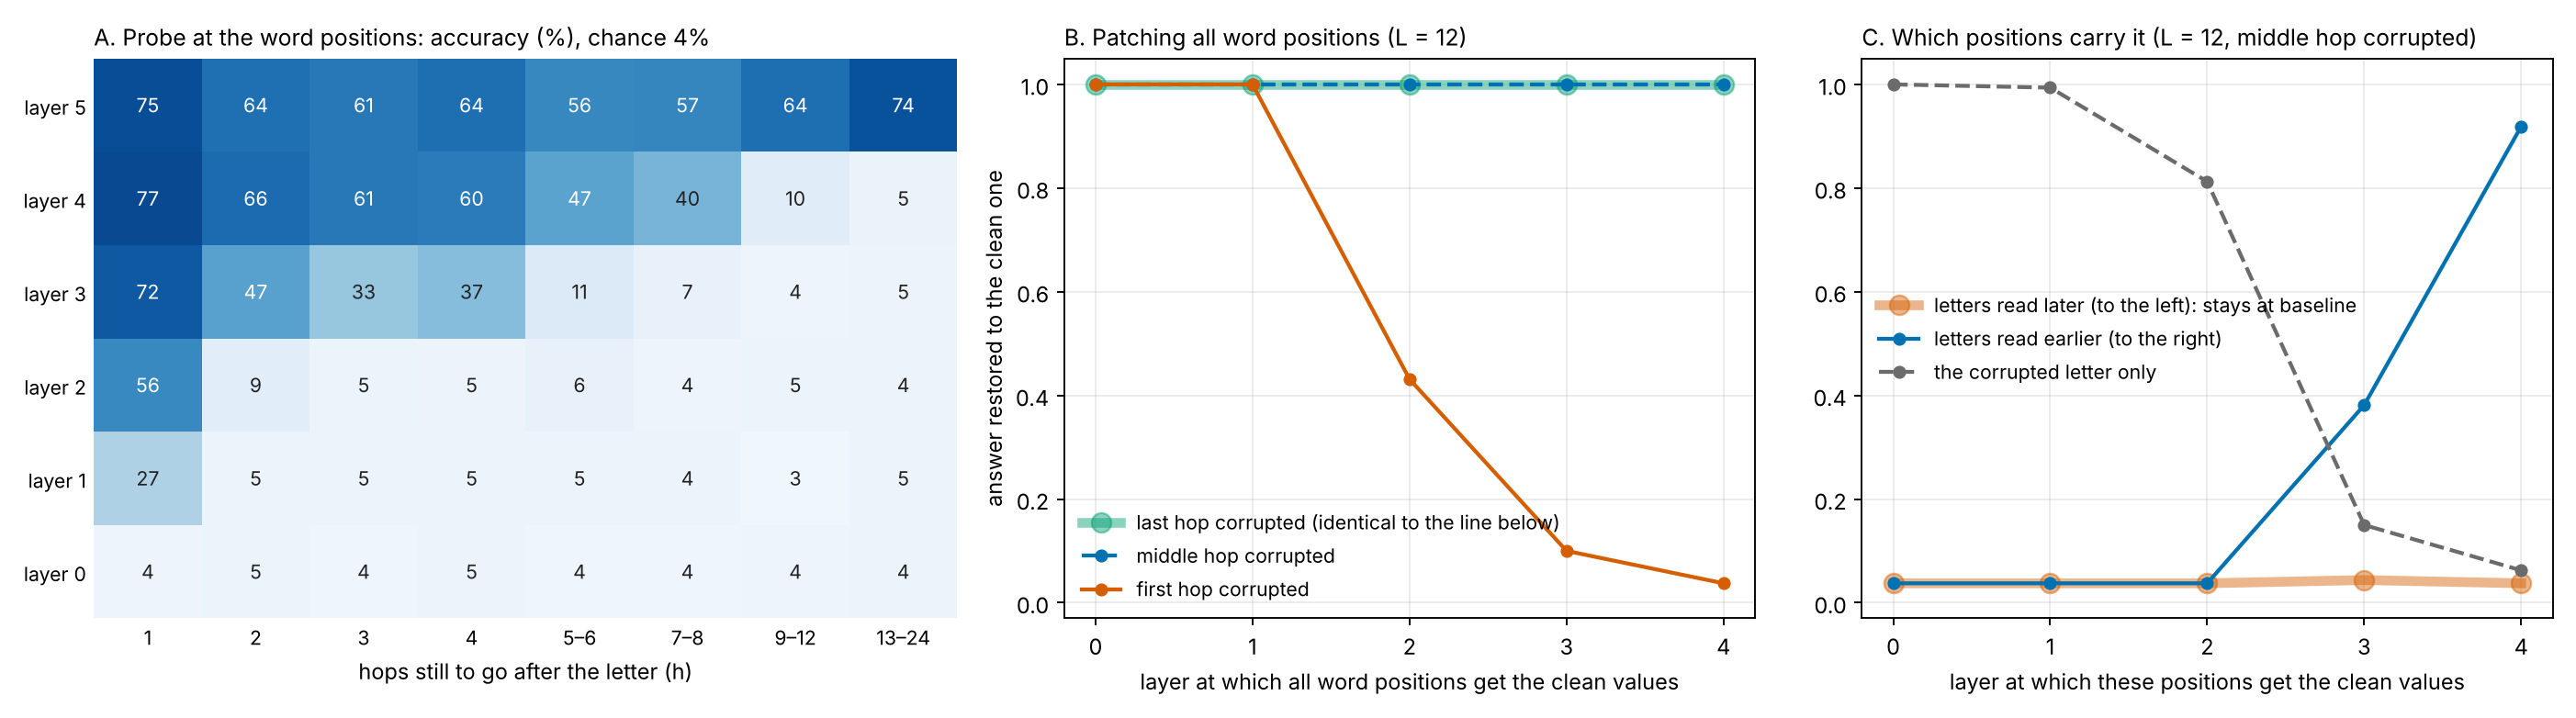
\includegraphics[width=1.00\linewidth]{fig_input_positions.png}\caption{Left: accuracy (\%) of a linear probe for the continuation of a chain, at the 25 word positions, by layer and by the number of hops $h$ still to go; chance is 4\%. Middle and right: activation patching (\S\,\ref{sec:3.10}) for planted chains of $L=12$ hops; “restored” is the share of words whose answer returns to the clean one.}\end{figure}

\lead{Setup} (\code{run\_\allowbreak{}input\_\allowbreak{}probes.\allowbreak{}py}, results in
\code{input\_\allowbreak{}probe\_\allowbreak{}results.\allowbreak{}json}, log in
\code{input\_\allowbreak{}probe\_\allowbreak{}log.\allowbreak{}txt}). Read a word right to left. A pointer that
leaves letter $t$ at endpoint $x$ continues through letters $t-1,\dots,0$ and ends at $\pi_{t-1}(x)$ after $h$
more hops. If the model composed chains by pointer jumping, the state of letter $t$ after layer $\ell$ would
carry $\pi_{t-1}(a_t)$ and $\pi_{t-1}(b_t)$ for chains of up to about $2^\ell$ remaining hops. So for every
layer $\ell$ (0 = embeddings, $\ell$ = after block $\ell$) I fit ridge probes from the residual stream at word
position $t$ to $\pi_{t-1}(a_t)$ and to $\pi_{t-1}(b_t)$ (25 classes each), \textbf{separately for each range of
$h$}, using only letters whose endpoint has that many hops to go. The rows are (word, position) pairs from 3,600
words: 1,200 planted words with $L=12$ and $s=9$, 1,200 planted with $L=20$ and $s=10$, and 1,200 natural words
over 25 points. Words are split 60/20/20 into train, validation (ridge strength) and test, so no word appears in
two parts. Input positions never see the outputs, so no teacher forcing is involved. A first version trained one
probe on all rows pooled; it was dominated by the many rows where the answer is the letter’s own endpoint
($h=0$) and showed nothing, so I report only the per-range probes.

Accuracy (\%) on test rows, chance 4\%:

{\small\nopagebreak[4]
\begin{longtable}{@{}l *{8}{r}@{}}
\toprule
\hdr{layer} & \hdr{$h=1$} & \hdr{2} & \hdr{3} & \hdr{4} & \hdr{5–6} & \hdr{7–8} & \hdr{9–12} & \hdr{13–24} \\
\midrule
\endfirsthead
\toprule
\hdr{layer} & \hdr{$h=1$} & \hdr{2} & \hdr{3} & \hdr{4} & \hdr{5–6} & \hdr{7–8} & \hdr{9–12} & \hdr{13–24} \\
\midrule
\endhead
\bottomrule
\endlastfoot
0 (embeddings) & 4 & 5 & 4 & 5 & 4 & 4 & 4 & 4 \\
1 & 27 & 5 & 5 & 5 & 5 & 4 & 3 & 5 \\
2 & 56 & 9 & 5 & 5 & 6 & 4 & 5 & 4 \\
3 & 72 & 47 & 33 & 37 & 11 & 7 & 4 & 5 \\
4 & 77 & 66 & 61 & 60 & 47 & 40 & 10 & 5 \\
5 & 75 & 64 & 61 & 64 & 56 & 57 & 64 & 74 \\
test rows & 8,650 & 4,569 & 2,199 & 1,076 & 1,234 & 986 & 1,661 & 1,589 \\
\end{longtable}}

Label-shuffle controls (training labels permuted across rows) give 3.3–5.2\% at layers 0, 4 and 5 for $h=1$, 5–6
and 13–24.

\begin{findbox}{What it shows}
\begin{itemize}
\item \lead{The reach of what is readable grows with depth.} At layers 1–2 only $h=1$ is readable. Readability
  extends to $h\le4$ at layer 3, to about $h\le8$ at layer 4, and to every $h$ I could test (up to 24) at layer
  5. Counting the hops covered, that is about 1, 1, 4, 8 and 13 or more at layers 1 to 5, which is a doubling
  pattern with some lag.
\item \lead{That is the pattern of log-depth composition, and it is a reason to take a depth limit seriously.}
  With about $2^\ell$ hops at layer $\ell$, five blocks would reach roughly 16 hops, close to where accuracy
  falls (\S\,\ref{sec:3.3}). This is a reading of the pattern; the probe does not show the algorithm. The
  elementary model has the same staircase and follows 80 hops (\S\,\ref{sec:3.11}), so the staircase alone is
  not that reason. \S\,\ref{sec:3.12} shows the doubling directly in the elementary model’s attention offsets
  and only partly in the general model’s. \S\,\ref{sec:3.14} shows a five-block model trained on long chains
  doing 24 hops, and \S\,\ref{sec:3.16} that its probes do not follow this staircase.
\item This is also where \S\,\ref{sec:3.6} left a gap: the query position holds the first few pointer states
  only, and the rest of the chain is held here, at the word positions.
\end{itemize}
\end{findbox}

\begin{limbox}{Limits}
\begin{itemize}
\item Natural words have at most about 9 remaining hops, so the bins with $h\ge9$ come only from my planted
  words. In those, the continuation at every hop letter of the long chain is the same point, the end of the
  chain, so these rows are less independent than their number suggests, and “decodable at layer 5” is weaker
  evidence for composition there than at small $h$.
\item A linear probe can fail to find information that is present in another form. The values of 3–5\% at the
  early layers mean that there is no linear code for this quantity there, not that there is no information.
\item Words are my own planted and natural words; I did not vary the distribution.
\item This is observational. \S\,\ref{sec:3.10} is the causal check.
\end{itemize}
\end{limbox}

\subsection{Activation patching at the word positions (Test 8)}\label{sec:3.10}
\lead{Setup} (\code{run\_\allowbreak{}patching.\allowbreak{}py}, results in
\code{patching\_\allowbreak{}results.\allowbreak{}json}, log in
\code{patching\_\allowbreak{}log.\allowbreak{}txt}).

\emph{The idea.} Damage the input in one place, then repair the model’s internal state in chosen places. If
putting the clean values back at some word positions, right after some block, undoes the damage, then the
information that decides the answer passes through those positions at that depth.

\begin{figure}[htbp]\centering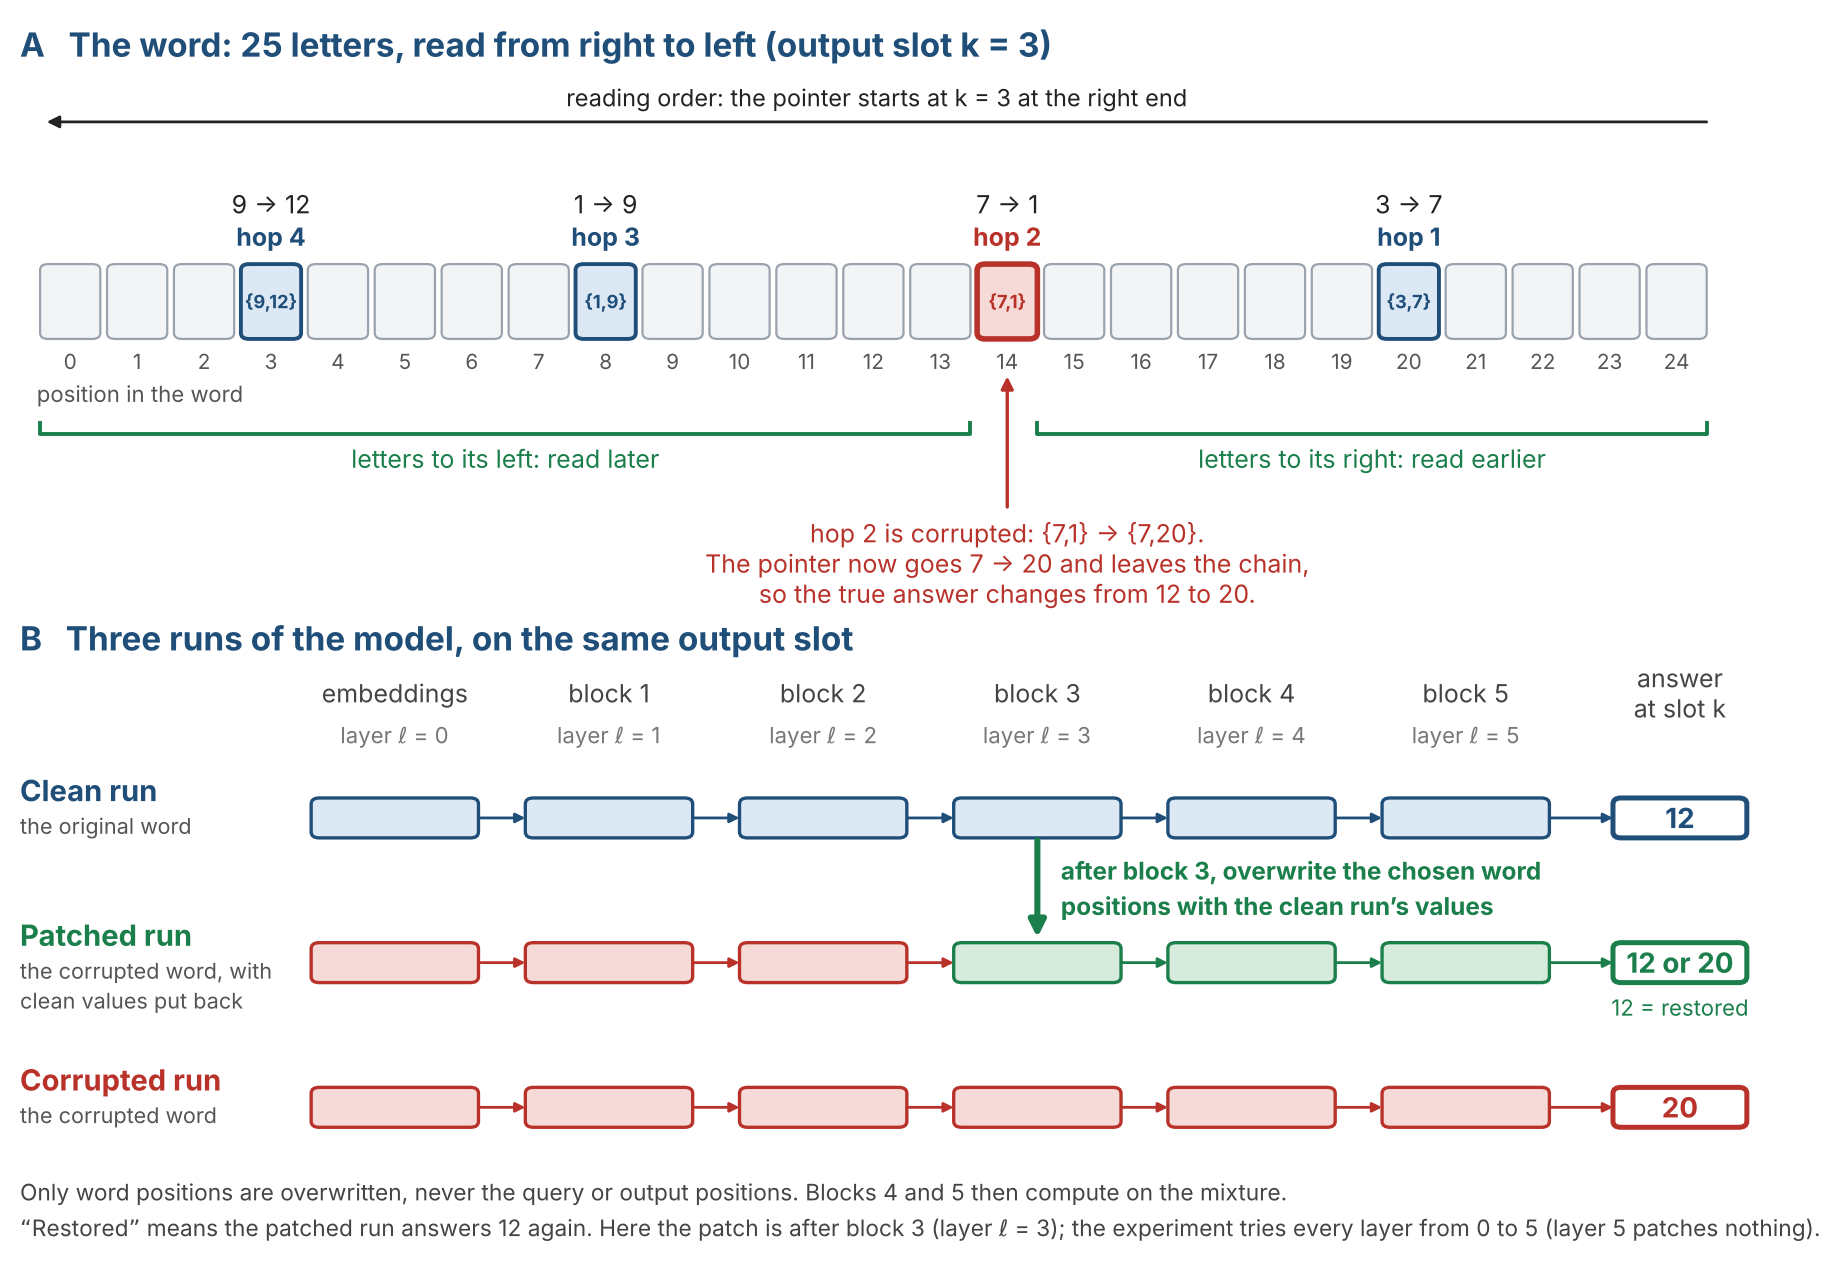
\includegraphics[width=1.00\linewidth]{fig_patching_setup.png}\caption{What the patching experiment does, for a word with $L=4$ hops (the real words have 25 letters and $L=8$, 12 or 16 hops). Top: the word, with the corrupted hop letter in red; “right” and “left” refer to that letter. Bottom: the three runs. The patched run is the corrupted run with clean values put back at chosen word positions after block $\ell$ ($\ell=3$ here).}\end{figure}

\emph{The four steps, for one output slot $k$ of one word.}

\begin{enumerate}
\item \lead{Clean word.} Take a planted word (\S\,\ref{sec:3.3}) in which the pointer of slot $k$ makes $L$ hops
  through $s=\min(L+1,10)$ distinct points, and keep it only if the model answers slot $k$ correctly. Call that
  answer $p_k$. The letters where the pointer moves are the \emph{hop letters} (the chain letters); all other
  letters are \emph{non-chain} letters. Number the hop letters $1,\dots,L$ in reading order, so hop 1 is the one
  nearest the right end, which the pointer meets first.
\item \lead{Corrupted word.} Pick one hop $j$. Its letter moves the pointer from $x_{j-1}$ to $x_j$. Replace it
  by a letter that moves the pointer from $x_{j-1}$ to $z$, where $z$ is a point not on the chain. The pointer
  now leaves the chain at hop $j$, and the true answer for slot $k$ becomes a different point $p^*_k$ (words
  where it does not change are dropped). In the figure ($L=4$, $k=3$) the hop letters
  $\{3,7\},\{7,1\},\{1,9\},\{9,12\}$ give $3\to7\to1\to9\to12$, so $p_k=12$. Replacing hop 2, $\{7,1\}$, by
  $\{7,20\}$ gives $3\to7\to20$, so $p^*_k=20$ (if a letter read later also contained 20, the pointer would
  carry on from there; the true answer is always recomputed from the corrupted word).
\item \lead{Two ordinary runs.} Run the model on the clean word and on the corrupted word. In both, the outputs
  fed back before slot $k$ are those of the clean word (teacher forcing), so the only difference between the
  runs is the word. Unpatched, the model follows the corrupted word, answering $p^*_k$, in 84–98\% of words (the
  “follows corrupted” column below), and answers $p_k$ in only 2–8\%.
\item \lead{Patched run.} Run the corrupted word again, but right after block $\ell$ overwrite the residual
  stream at a chosen set of word positions with the values from the clean run. The later blocks then compute on
  this mixture. The query and output positions are never overwritten. A word counts as \textbf{restored} if the
  prediction at slot $k$ is $p_k$ again. Here $\ell=0$ means the embeddings (before block 1) and $\ell$ means
  after block $\ell$.
\end{enumerate}

\emph{Which positions are overwritten.} Within the word every position can attend to every other one, so the
corruption can reach any of them. I try six sets:

\begin{itemize}
\item all 25 word positions;
\item the chain letters (all hop letters);
\item the letters to the right of the corrupted one (read earlier in the chase);
\item the letters to the left of it (read later);
\item the corrupted letter alone;
\item the non-chain letters (a control).
\end{itemize}

\emph{Reference points.} Patching all word positions at layer 0 gives back the clean word exactly, so it must
restore every word (the column headed 0 below). Patching at layer 5 changes nothing, because no later block
reads the word positions; it is the unpatched run, restored in 2–8\% of words.

\emph{What was run.} The corrupted hop was the first (hop 1), the middle (hop $L/2+1$) or the last (hop $L$),
for chains with $L=8$, 12 and 16, with 143–160 words each. Every table cell below is the share of those words
that are restored; the columns are the layer $\ell$ at which the patch is made (0–4).

\Needspace*{16\baselineskip}Patching \textbf{all 25 word positions} at layer $\ell$ (columns 0–4), by corrupted
hop:

{\small\nopagebreak[4]
\begin{longtable}{@{}r l r r *{5}{r}@{}}
\toprule
& & & & \multicolumn{5}{c}{\hdr{restored when patching at layer $\ell$}} \\
\cmidrule(lr){5-9}
\hdr{$L$} & \hdr{corrupted hop} & \hdr{words} & \hdr{follows corrupted} & \hdr{0} & \hdr{1} & \hdr{2} & \hdr{3} & \hdr{4} \\
\midrule
\endfirsthead
\toprule
& & & & \multicolumn{5}{c}{\hdr{restored when patching at layer $\ell$}} \\
\cmidrule(lr){5-9}
\hdr{$L$} & \hdr{corrupted hop} & \hdr{words} & \hdr{follows corrupted} & \hdr{0} & \hdr{1} & \hdr{2} & \hdr{3} & \hdr{4} \\
\midrule
\endhead
\bottomrule
\endlastfoot
8 & first & 160 & 0.96 & 1.00 & 1.00 & 0.51 & 0.10 & 0.05 \\*
8 & middle & 160 & 0.95 & 1.00 & 1.00 & 1.00 & 1.00 & 1.00 \\*
8 & last & 160 & 0.95 & 1.00 & 1.00 & 1.00 & 1.00 & 1.00 \\
\addlinespace[4pt]
12 & first & 160 & 0.97 & 1.00 & 1.00 & 0.43 & 0.10 & 0.04 \\*
12 & middle & 160 & 0.96 & 1.00 & 1.00 & 1.00 & 1.00 & 1.00 \\*
12 & last & 160 & 0.95 & 1.00 & 1.00 & 1.00 & 1.00 & 1.00 \\
\addlinespace[4pt]
16 & first & 143 & 0.98 & 1.00 & 1.00 & 0.33 & 0.08 & 0.03 \\*
16 & middle & 143 & 0.93 & 1.00 & 1.00 & 1.00 & 1.00 & 1.00 \\*
16 & last & 143 & 0.84 & 1.00 & 1.00 & 1.00 & 1.00 & 1.00 \\
\end{longtable}}

\Needspace*{16\baselineskip}Patching \textbf{subsets} of positions, $L=12$, restored at layer 0 / 1 / 2 / 3 / 4:

{\small\nopagebreak[4]
\begin{longtable}{@{}l >{\raggedright\arraybackslash}p{5.4cm} *{5}{r}@{}}
\toprule
\hdr{corrupted hop} & \hdr{patched positions} & \multicolumn{5}{c}{\hdr{restored when patching at layer $\ell$}} \\
\cmidrule(lr){3-7}
 & & \hdr{0} & \hdr{1} & \hdr{2} & \hdr{3} & \hdr{4} \\
\midrule
\endfirsthead
\toprule
\hdr{corrupted hop} & \hdr{patched positions} & \multicolumn{5}{c}{\hdr{restored when patching at layer $\ell$}} \\
\cmidrule(lr){3-7}
 & & \hdr{0} & \hdr{1} & \hdr{2} & \hdr{3} & \hdr{4} \\
\midrule
\endhead
\bottomrule
\endlastfoot
\textbf{middle} & chain letters & 1.00 & 1.00 & 1.00 & 1.00 & 1.00 \\*
 & letters to the right (read earlier) & .04 & .04 & .04 & .38 & .92 \\*
 & letters to the left (read later) & \multicolumn{5}{c}{.04 at every layer} \\*
 & the corrupted letter & 1.00 & .99 & .81 & .15 & .06 \\*
 & non-chain letters & \multicolumn{5}{c}{.04 at every layer} \\
\addlinespace[4pt]
\textbf{last} & chain letters & 1.00 & 1.00 & 1.00 & 1.00 & 1.00 \\*
 & letters to the right (read earlier) & .04 & .04 & .77 & 1.00 & 1.00 \\*
 & letters to the left (read later) & \multicolumn{5}{c}{.04 at every layer} \\*
 & the corrupted letter & 1.00 & 1.00 & .35 & .04 & .04 \\*
 & non-chain letters & \multicolumn{5}{c}{.04 at every layer} \\
\addlinespace[4pt]
\textbf{first} & chain letters & 1.00 & 1.00 & .40 & .07 & .04 \\*
 & letters to the right (read earlier) & \multicolumn{5}{c}{.03 at every layer} \\*
 & letters to the left (read later) & \multicolumn{5}{c}{.03 at every layer} \\*
 & the corrupted letter & 1.00 & .98 & .23 & .06 & .04 \\*
 & non-chain letters & \multicolumn{5}{c}{.03 at every layer} \\
\end{longtable}}

\begin{findbox}{What it shows}
\begin{itemize}
\item \lead{Late hops are read from the word positions in the last block.} For a middle or last hop, patching
  all word positions even at layer 4, which leaves block 5 as the only reader, brings back the clean answer in
  every word, although the query position’s own residual stream after block 4 was computed from the corrupted
  word. Whatever the query took in during blocks 1–4 about these hops does not decide the answer.
\item \lead{The first hops are different.} Corrupting the first hop is not repaired by clean word positions from
  layer 2 or 3 on (33–51\% after block 2, 8–10\% after block 3), because the query position has already read it:
  that is the part of the chain the query holds itself (\S\,\ref{sec:3.6}).
\item \lead{The corrupted letter’s effect travels to the letters read before it.} Clean activations at the
  letters to its right (read earlier in the chase) restore the answer, from layer 2 for the last hop and from
  layer 3 for a middle hop, while clean activations at the letters to its left (read later) restore nothing at
  any layer. This is the direction in which the continuation probes of \S\,\ref{sec:3.9} would be built: each
  letter learns where the chain beyond it leads.
\item The corrupted letter’s own state carries it only through about layer 2, after which the information has
  moved to other positions. Non-chain letters never matter (control).
\end{itemize}
\end{findbox}

\begin{limbox}{Limits}
143–160 words per cell, chains of at most 16 hops (at $L=20$ the model is right only about half the time, so
there is no clean baseline to restore), one corruption type, and positions are patched all at once rather than
one head or one layer component at a time. “Restored” is the share of words whose prediction equals the clean
answer; the unpatched baseline is 2–8\%.
\end{limbox}

\subsection{Probes and patching at the word positions of the elementary model (Tests 9 and 10)}\label{sec:3.11}
\begin{figure}[htbp]\centering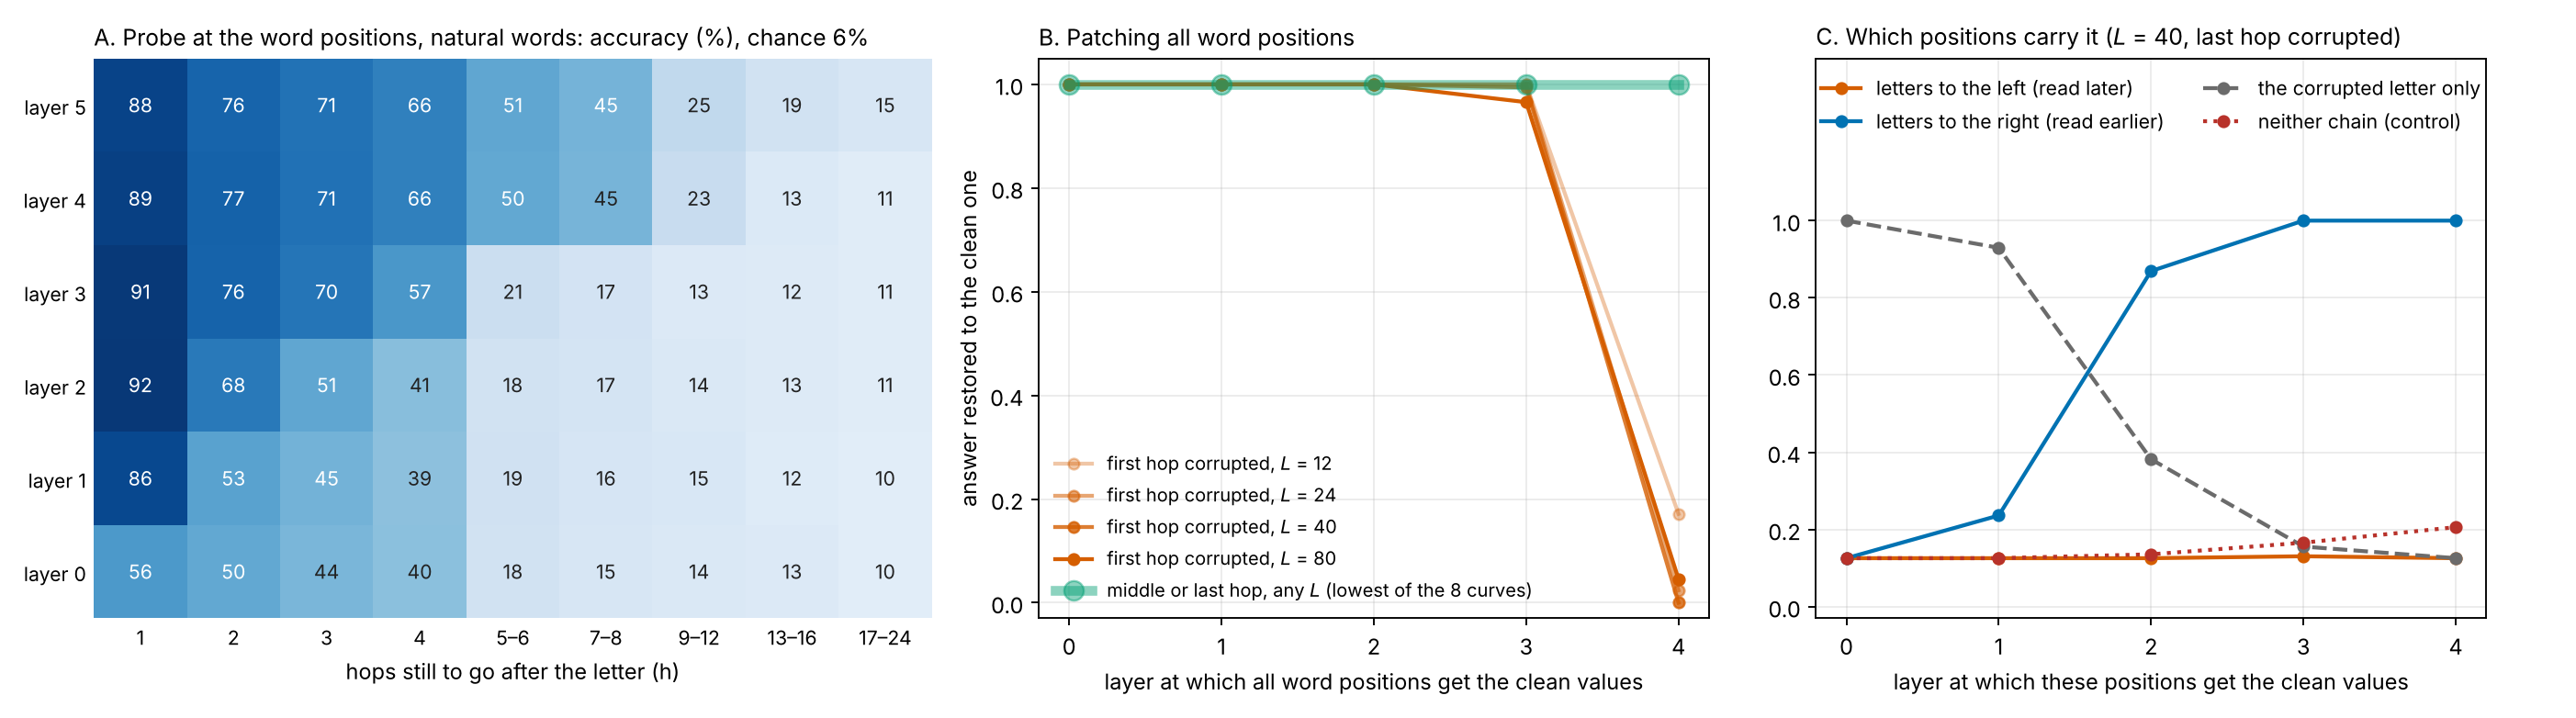
\includegraphics[width=1.00\linewidth]{fig_input_positions_elem.png}\caption{Left: accuracy (\%) of a linear probe for the continuation of a chain at the 120 word positions of the elementary model, natural words, by layer and by the number of hops $h$ still to go; chance is 6\%. Middle: activation patching of all word positions, for planted chains of $L=12$ to 80 hops. Right: which positions carry the answer, for $L=40$ with the last hop corrupted. “Restored” is the share of words whose answer returns to the clean one.}\end{figure}

\lead{Why.} The elementary model follows chases of up to 80 hops (\S\,\ref{sec:3.8}), five times as far as the
general model. In \S\,\ref{sec:3.9} I read the general model’s staircase of readable continuations (about 1, 1,
4, 8 and 13 or more hops at layers 1 to 5) as log-depth composition, which would cap five blocks near 16 hops.
If the elementary model shows the same staircase and still follows 80 hops, the staircase alone cannot be what
sets a model’s hop limit. So I ran the tests of \S\,\ref{sec:3.9} and \S\,\ref{sec:3.10} on it.

{\raggedright \lead{Setup}
(\code{run\_\allowbreak{}input\_\allowbreak{}probes\_\allowbreak{}elem.\allowbreak{}py},
\code{run\_\allowbreak{}patching\_\allowbreak{}elem.\allowbreak{}py}; results in
\code{input\_\allowbreak{}probe\_\allowbreak{}elem\_\allowbreak{}results.\allowbreak{}json} and
\code{patching\_\allowbreak{}elem\_\allowbreak{}results.\allowbreak{}json}, logs in
\code{input\_\allowbreak{}probe\_\allowbreak{}elem\_\allowbreak{}log.\allowbreak{}txt} and
\code{patching\_\allowbreak{}elem\_\allowbreak{}log.\allowbreak{}txt}). The designs are those of
\S\,\ref{sec:3.9} (ridge probes per range of remaining hops) and \S\,\ref{sec:3.10} (corrupt one hop letter,
patch clean activations back, teacher forcing with the clean outputs; the four steps are described there). The
elementary letters force these changes:\par}

\begin{itemize}
\item A word has 120 letters. Token $\tau\ge1$ swaps positions $\tau-1$ and $\tau$, so a letter’s endpoints are
  $a=\tau-1$ and $b=\tau$, and there are 16 points, so the probes have 16 classes (chance 6\%). Identity letters
  (token 0) have no endpoints and are left out of the probes.
\item Probes: 1,350 words, namely 450 natural words (120 uniform letters over the 16 tokens, as in the real test
  file) and 450 planted words each with $L=40$ and with $L=80$ hops over a window of width 8, which supply the
  long ranges. The hop ranges are extended to 25–48 and 49 or more. Words are split 60/20/20 into train,
  validation and test as in \S\,\ref{sec:3.9}. The main table uses the natural words only, trained and tested
  within them.
\item Corruption: the hop letter that moves the pointer from $x_{j-1}$ to $x_j$ is replaced by the letter that
  moves it to the other neighbour, $z=2x_{j-1}-x_j$. If $z$ is outside 0 to 15 no such letter exists and the
  word is skipped (19 to 33 of 200 words when the first hop is corrupted, at most 6 otherwise). The corrupted
  pointer then follows its own chain of hop letters, which differs from the clean chain, so besides the clean
  chain I also patch the corrupted pointer’s hop letters, and the control “neither chain” excludes both.
\item Patching: planted words with $L=12$, 24, 40 and 80 hops over width 8; the first, middle (hop $L/2+1$) and
  last hop corrupted; 200 words per $L$ (the model is right on all 200 clean words at every $L$), 167 to 200 per
  cell after skipping. A faster but equivalent computation recomputes only the blocks after the patched layer. I
  checked it against the full forward pass of \S\,\ref{sec:3.10} on 30 words: identical predictions, logits
  equal to $2\times10^{-7}$.
\end{itemize}

Accuracy (\%) on test rows of the probe, natural words only. Layer 0 is the baseline to compare with, because
the token and position alone already give 40–56\% at $h\le4$, where the endpoint is only a few steps from where
it started:

{\small\nopagebreak[4]
\begin{longtable}{@{}l *{9}{r}@{}}
\toprule
\hdr{layer} & \hdr{$h=1$} & \hdr{2} & \hdr{3} & \hdr{4} & \hdr{5–6} & \hdr{7–8} & \hdr{9–12} & \hdr{13–16} & \hdr{17–24} \\
\midrule
\endfirsthead
\toprule
\hdr{layer} & \hdr{$h=1$} & \hdr{2} & \hdr{3} & \hdr{4} & \hdr{5–6} & \hdr{7–8} & \hdr{9–12} & \hdr{13–16} & \hdr{17–24} \\
\midrule
\endhead
\bottomrule
\endlastfoot
0 (embeddings) & 56 & 50 & 44 & 40 & 18 & 15 & 14 & 13 & 10 \\
1 & 86 & 53 & 45 & 39 & 19 & 16 & 15 & 12 & 10 \\
2 & 92 & 68 & 51 & 41 & 18 & 17 & 14 & 13 & 11 \\
3 & 91 & 76 & 70 & 57 & 21 & 17 & 13 & 12 & 11 \\
4 & 89 & 77 & 71 & 66 & 50 & 45 & 23 & 13 & 11 \\
5 & 88 & 76 & 71 & 66 & 51 & 45 & 25 & 19 & 15 \\
test rows & 1,424 & 1,423 & 1,420 & 1,418 & 2,811 & 2,700 & 4,395 & 2,266 & 746 \\
\end{longtable}}

Label-shuffle controls (training labels permuted across rows) give 5.8–7.5\% at layer 0 and 6.0–9.3\% at layers
4 and 5, for $h=1$, 5–6, 13–24 and 25–48.

Long ranges exist only in my planted words (natural words have at most about 24 remaining hops). Accuracy (\%)
there, trained and tested within each set, for layers 0, 4 and 5:

{\small\nopagebreak[4]
\begin{longtable}{@{}l l *{6}{r}@{}}
\toprule
\hdr{planted words} & \hdr{layer} & \hdr{9–12} & \hdr{13–16} & \hdr{17–24} & \hdr{25–32} & \hdr{33–48} & \hdr{49+} \\
\midrule
\endfirsthead
\toprule
\hdr{planted words} & \hdr{layer} & \hdr{9–12} & \hdr{13–16} & \hdr{17–24} & \hdr{25–32} & \hdr{33–48} & \hdr{49+} \\
\midrule
\endhead
\bottomrule
\endlastfoot
$L=40$ & 0 & 15 & 13 & 12 & 10 & 16 & – \\
 & 4 & 26 & 16 & 14 & 15 & 17 & – \\
 & 5 & 28 & 18 & 23 & 36 & 42 & – \\
 & test rows & 3,642 & 1,821 & 1,313 & 729 & 630 & – \\
$L=80$ & 0 & 18 & 16 & 15 & 17 & 16 & 11 \\
 & 4 & 33 & 25 & 20 & 16 & 14 & 16 \\
 & 5 & 33 & 25 & 32 & 54 & 66 & 66 \\
 & test rows & 2,491 & 1,651 & 1,704 & 875 & 1,465 & 2,821 \\
\end{longtable}}

\Needspace*{16\baselineskip}Patching \textbf{all 120 word positions} at layer $\ell$ (columns 0–4), by corrupted
hop (“follows corrupted” is the unpatched model’s share of answers equal to the corrupted word’s):

{\small\nopagebreak[4]
\begin{longtable}{@{}r l r r *{5}{r}@{}}
\toprule
& & & & \multicolumn{5}{c}{\hdr{restored when patching at layer $\ell$}} \\
\cmidrule(lr){5-9}
\hdr{$L$} & \hdr{corrupted hop} & \hdr{words} & \hdr{follows corrupted} & \hdr{0} & \hdr{1} & \hdr{2} & \hdr{3} & \hdr{4} \\
\midrule
\endfirsthead
\toprule
& & & & \multicolumn{5}{c}{\hdr{restored when patching at layer $\ell$}} \\
\cmidrule(lr){5-9}
\hdr{$L$} & \hdr{corrupted hop} & \hdr{words} & \hdr{follows corrupted} & \hdr{0} & \hdr{1} & \hdr{2} & \hdr{3} & \hdr{4} \\
\midrule
\endhead
\bottomrule
\endlastfoot
12 & first & 181 & 0.99 & 1.00 & 1.00 & 1.00 & 1.00 & .17 \\*
12 & middle & 200 & 0.94 & 1.00 & 1.00 & 1.00 & 1.00 & 1.00 \\*
12 & last & 196 & 0.94 & 1.00 & 1.00 & 1.00 & 1.00 & 1.00 \\
\addlinespace[4pt]
24 & first & 167 & 0.99 & 1.00 & 1.00 & 1.00 & 1.00 & .02 \\*
24 & middle & 196 & 0.91 & 1.00 & 1.00 & 1.00 & 1.00 & 1.00 \\*
24 & last & 200 & 0.90 & 1.00 & 1.00 & 1.00 & 1.00 & 1.00 \\
\addlinespace[4pt]
40 & first & 176 & 0.98 & 1.00 & 1.00 & 1.00 & .99 & .00 \\*
40 & middle & 196 & 0.86 & 1.00 & 1.00 & 1.00 & 1.00 & 1.00 \\*
40 & last & 199 & 0.86 & 1.00 & 1.00 & 1.00 & 1.00 & 1.00 \\
\addlinespace[4pt]
80 & first & 175 & 0.92 & 1.00 & 1.00 & 1.00 & .97 & .05 \\*
80 & middle & 194 & 0.71 & 1.00 & 1.00 & 1.00 & 1.00 & 1.00 \\*
80 & last & 196 & 0.69 & 1.00 & 1.00 & 1.00 & 1.00 & 1.00 \\
\end{longtable}}

\Needspace*{16\baselineskip}Patching \textbf{subsets} of positions, $L=40$, restored at layer 0 / 1 / 2 / 3 / 4:

{\small\nopagebreak[4]
\begin{longtable}{@{}l >{\raggedright\arraybackslash}p{5.4cm} *{5}{r}@{}}
\toprule
\hdr{corrupted hop} & \hdr{patched positions} & \multicolumn{5}{c}{\hdr{restored when patching at layer $\ell$}} \\
\cmidrule(lr){3-7}
 & & \hdr{0} & \hdr{1} & \hdr{2} & \hdr{3} & \hdr{4} \\
\midrule
\endfirsthead
\toprule
\hdr{corrupted hop} & \hdr{patched positions} & \multicolumn{5}{c}{\hdr{restored when patching at layer $\ell$}} \\
\cmidrule(lr){3-7}
 & & \hdr{0} & \hdr{1} & \hdr{2} & \hdr{3} & \hdr{4} \\
\midrule
\endhead
\bottomrule
\endlastfoot
\textbf{middle} & chain letters & 1.00 & 1.00 & .99 & .99 & .99 \\*
 & corrupted pointer’s chain letters & 1.00 & .98 & .90 & .91 & .87 \\*
 & letters to the right (read earlier) & .13 & .20 & .40 & .57 & .77 \\*
 & letters to the left (read later) & .13 & .15 & .53 & .68 & .45 \\*
 & the corrupted letter & 1.00 & .92 & .44 & .23 & .15 \\*
 & neither chain & .13 & .13 & .14 & .15 & .15 \\
\addlinespace[4pt]
\textbf{last} & chain letters & \multicolumn{5}{c}{1.00 at every layer} \\*
 & corrupted pointer’s chain letters & \multicolumn{5}{c}{1.00 at every layer} \\*
 & letters to the right (read earlier) & .13 & .24 & .87 & 1.00 & 1.00 \\*
 & letters to the left (read later) & \multicolumn{5}{c}{.13 at every layer} \\*
 & the corrupted letter & 1.00 & .93 & .38 & .16 & .13 \\*
 & neither chain & .13 & .13 & .14 & .17 & .21 \\
\addlinespace[4pt]
\textbf{first} & chain letters & 1.00 & 1.00 & .99 & .58 & .00 \\*
 & corrupted pointer’s chain letters & 1.00 & .95 & .72 & .52 & .00 \\*
 & letters to the right (read earlier) & \multicolumn{5}{c}{.00 at every layer} \\*
 & letters to the left (read later) & .00 & .02 & .49 & .84 & .00 \\*
 & the corrupted letter & 1.00 & .94 & .43 & .06 & .00 \\*
 & neither chain & \multicolumn{5}{c}{.00 at every layer} \\
\end{longtable}}

\begin{findbox}{What it shows}
\begin{itemize}
\item \lead{The probes show the same doubling staircase.} On natural words the readable reach (accuracy clearly
  above the layer-0 row) is $h=1$ at layer 1 (86\% against 56\%), $h\le2$ at layer 2 (68\% against 50\%),
  $h\le4$ at layer 3 (70\% at $h=3$ and 57\% at $h=4$, against 44\% and 40\%), $h\le8$ at layer 4 (50\% and 45\%
  at $h=5$–6 and 7–8, against 18\% and 15\%), and only partly beyond at layer 5 (25\% at $h=9$–12 and 19\% at
  13–16, against 14\% and 13\%; nothing at 17–24). That is about 1, 2, 4, 8 and 12 hops at layers 1 to 5,
  against 1, 1, 4, 8 and 13 or more for the general model (\S\,\ref{sec:3.9}): a doubling pattern with a short
  last step.
\item \lead{Yet this model follows 80 hops, so the staircase alone does not set the hop limit.} No word position
  holds more than about 8 to 12 hops of continuation at any layer in natural words, and a chase of 80 hops is
  still followed (\S\,\ref{sec:3.8}). Patching agrees that the first hops are not taken in later for longer
  chains: with the first hop corrupted, restoring all word positions works through layer 3 (0.97–1.00 at every
  $L$ from 12 to 80) and fails after block 4 (0.00–0.17). Whatever the elementary model does with long chains,
  it is not capped by a per-position reach of about $2^\ell$. This weakens the argument I drew from
  \S\,\ref{sec:3.9} for the general model (\S\,\ref{sec:5} item 9); it does not show that the general model is
  not depth-limited, because the two tasks differ (a hop moves the pointer by one place, inside a window of at
  most 11 positions in training).
\item \lead{Late hops are still read from the word positions in the last block.} For a middle or last hop,
  patching all word positions after block 4 restores the clean answer in every word (1.00 at every $L$ from 12
  to 80), and the chain letters alone do almost as well (0.93–1.00), although the query position’s own state was
  computed from the corrupted word. This is the same as in \S\,\ref{sec:3.10}.
\item \lead{One difference from the general model: the letters read later also carry it.} For the first and the
  middle hop, patching only the letters to the left of the corrupted one (read later) restores the answer: for
  the first hop 0.49 after block 2 and 0.84 after block 3, for the middle hop 0.53, 0.68 and 0.45 after blocks
  2, 3 and 4 ($L=40$). In \S\,\ref{sec:3.10} this set restored nothing in any condition. The right side restores
  it, as in \S\,\ref{sec:3.10}, when it holds hop letters (middle or last hop; last hop, $L=40$: 0.87 after
  block 2, 1.00 after blocks 3 and 4); the left side does so only in this model (first or middle hop), and not
  when it holds no hop letters (last hop). The corrupted letter’s own state carries the answer through layer 1
  (0.92–0.93) and not after layer 2 (0.38–0.44), and the “neither chain” control stays near the unpatched level
  (0.13 to 0.21 at most).
\item \lead{At $L=80$ the model partly ignores a corrupted middle or last hop.} Unpatched, 25–26\% of those
  words still get the clean answer and only 69–71\% follow the corrupted word (86–94\% at $L\le40$). This is
  like the general model at $L=20$ (\S\,\ref{sec:3.7}), and it puts a floor of 25\% under the restoration rates
  in those rows.
\end{itemize}
\end{findbox}

\begin{limbox}{Limits}
\begin{itemize}
\item The longest ranges ($h\ge13$ at layer 5 and the 25-or-more bins) exist only in planted words, which are
  unlike natural ones: at $L=80$ two thirds of the letters are hops of one chain. All rows of one chain share a
  label, and at layer 5 accuracy there jumps (54–66\% at 25–48 hops, against 14–16\% at layer 4). Nothing reads
  the word positions after block 5, and the number of hops is confounded with the position of the letter in the
  word: for letters in the left half, $t<60$, layer 4 already reads about 13–16 hops (43\%) and layer 5 up to 48
  (70\%). I do not read the layer-5 jump as composition.
\item The staircase is read from natural words, where $h\ge13$ has few rows (2,266 and 746 test rows) and the
  layer-0 baseline is not chance. A linear probe can miss information that is present in another form.
\item One corruption type (the other neighbour); the corrupted pointer then follows its own hops, which the
  general-model design (a fresh point) avoids. Width 8 only, 167–200 words per cell, positions patched all at
  once rather than one head or one component at a time.
\item Probes are observational; the patching is the causal check. Neither says how the elementary model composes
  80 hops. That needs, for example, attention patterns or head-level patching at long $L$ (\S\,\ref{sec:6}).
  \S\,\ref{sec:3.12} adds attention patterns and single-head ablation; it does not find the mechanism either,
  and head-level patching is still open.
\end{itemize}
\end{limbox}

\subsection{Attention patterns and single-head ablation (Tests 11 and 12)}\label{sec:3.12}
\begin{figure}[htbp]\centering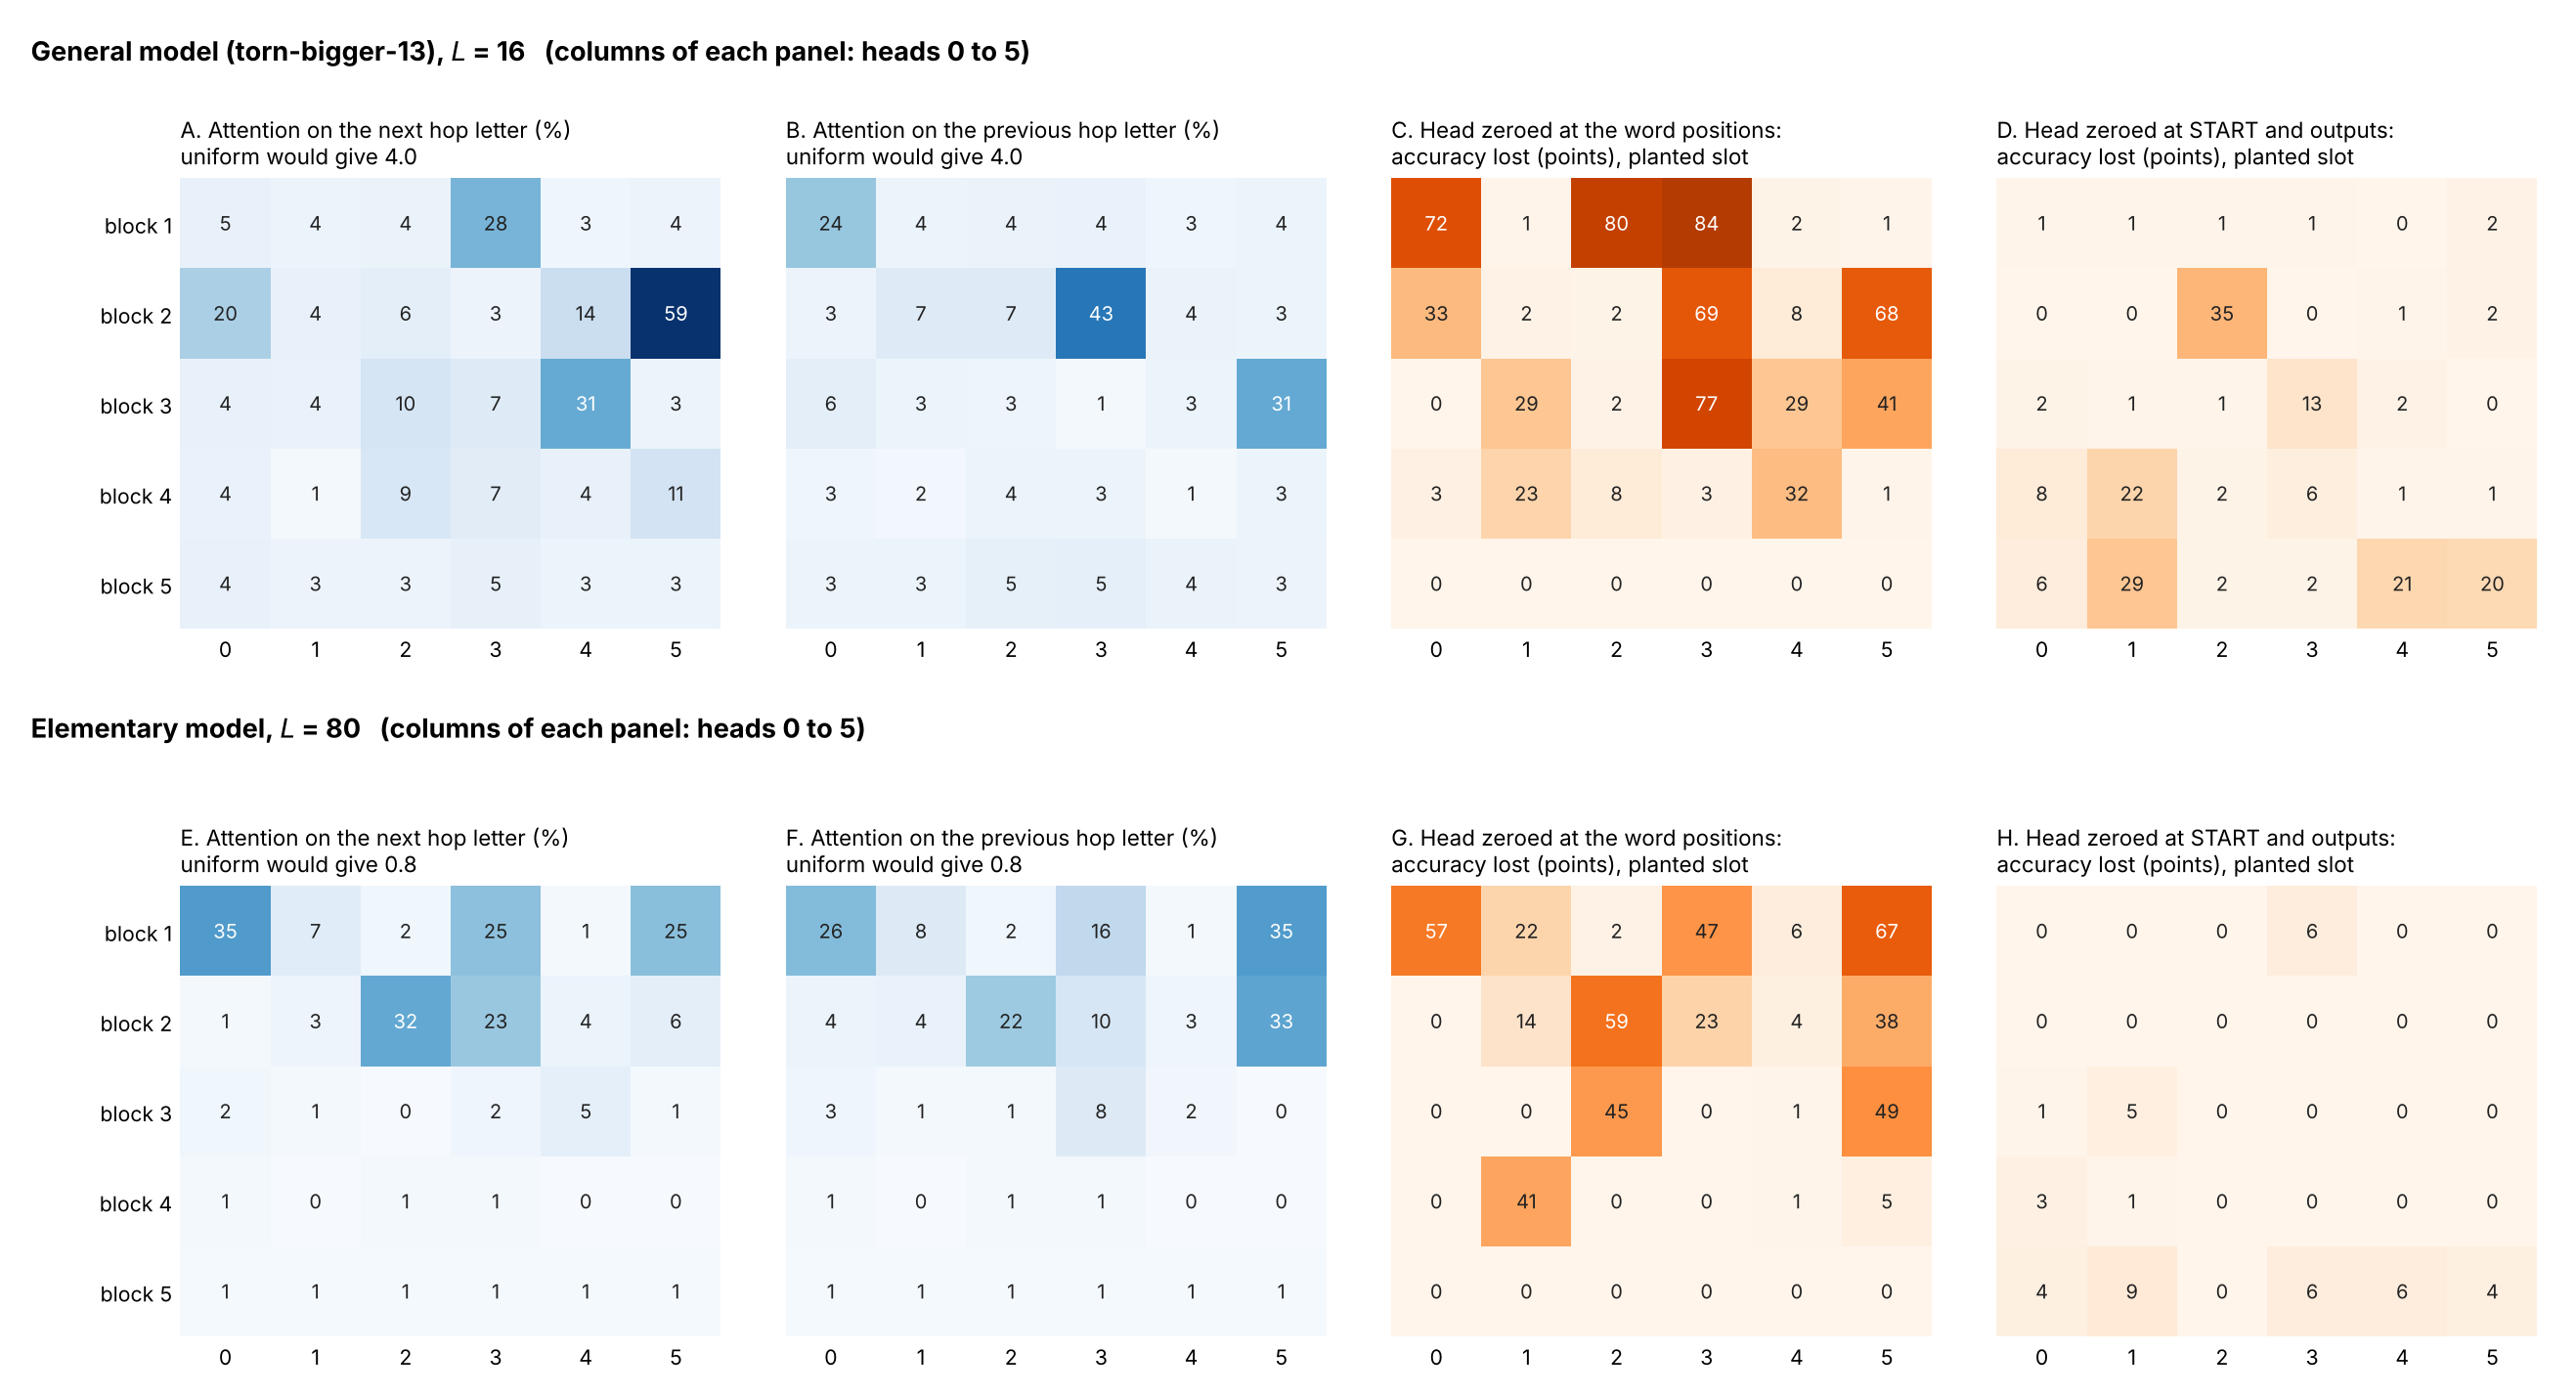
\includegraphics[width=1.00\linewidth]{fig_attention_heads.png}\caption{Attention and ablation by head, planted chains. Top row: the general model, $L=16$. Bottom row: the elementary model, $L=80$. In each panel the rows are blocks 1 to 5 and the columns are heads 0 to 5. A, B, E, F: the share (\%) of a hop letter’s attention that falls on the next hop letter (read later, to its left) and on the previous hop letter (read earlier, to its right), averaged over the hop letters of the chain; uniform attention would give 4.0\% (general) and 0.8\% (elementary). C, D, G, H: accuracy lost at the planted slot (percentage points) when one head’s output is set to zero at the word positions (C, G) or at START and the output positions (D, H).}\end{figure}

\begin{figure}[htbp]\centering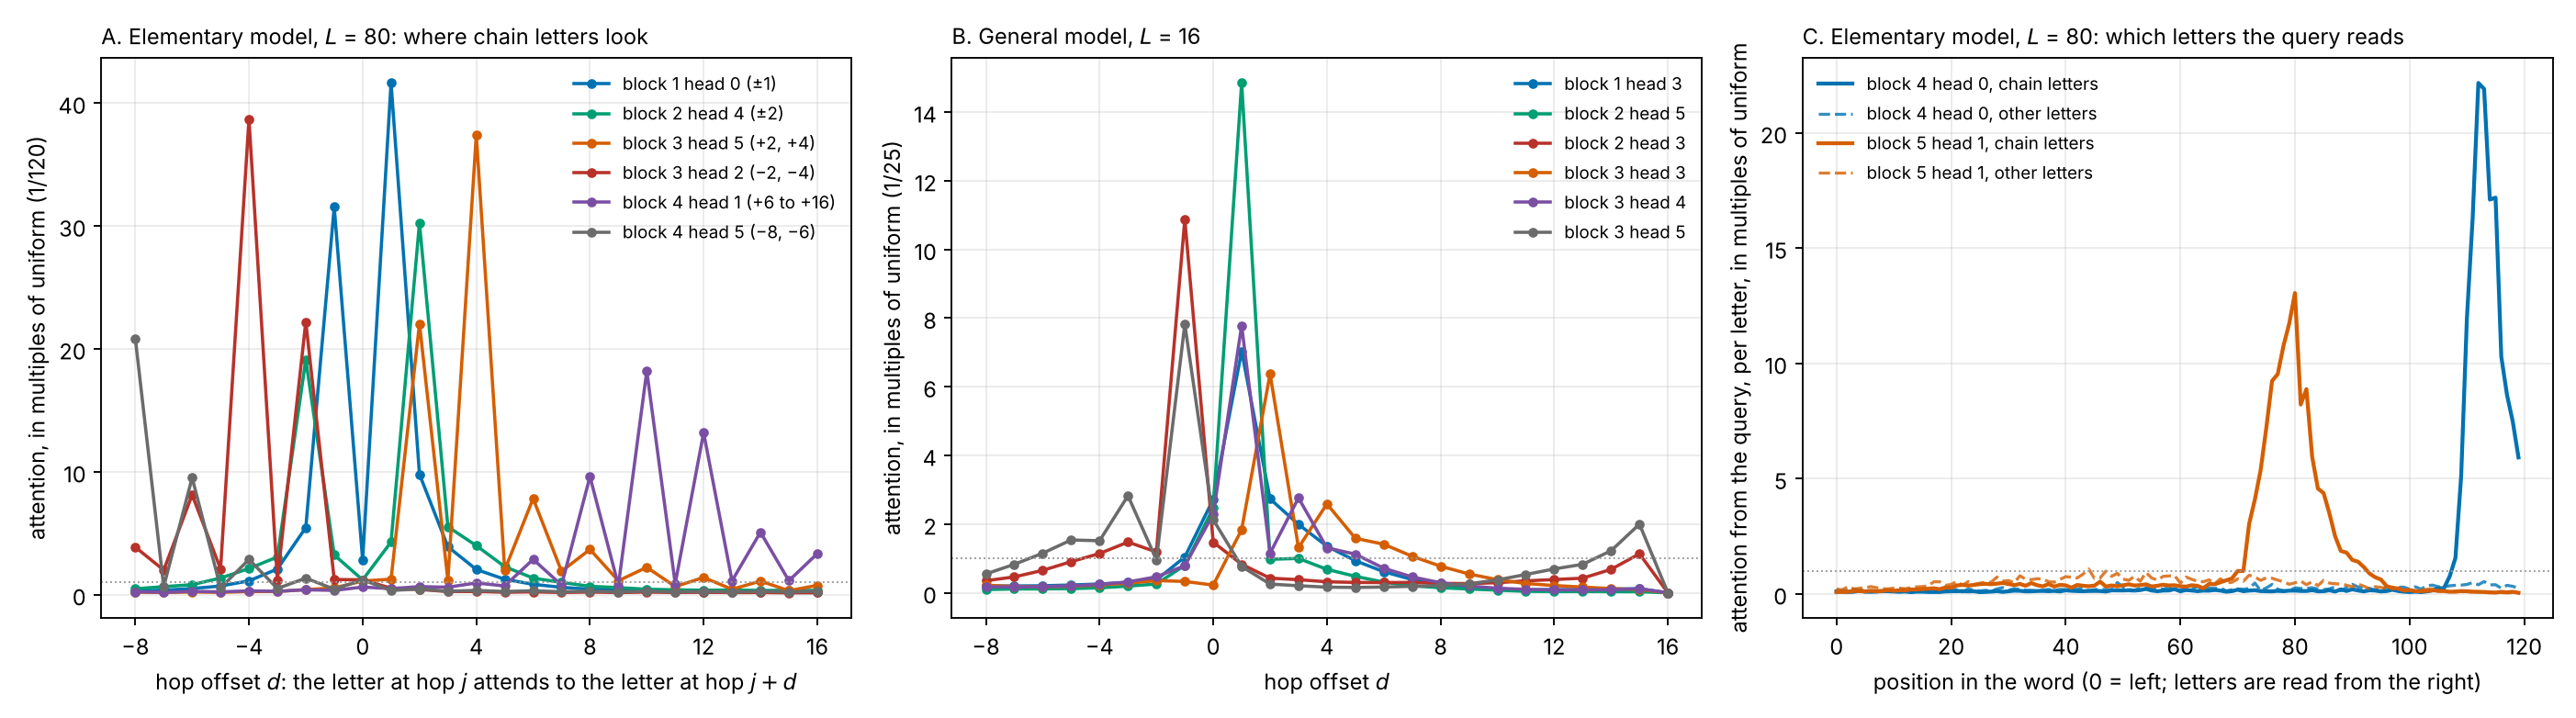
\includegraphics[width=1.00\linewidth]{fig_attention_profiles.png}\caption{Left: the elementary model’s heads at the word positions, $L=80$. A hop letter’s attention to the letter $d$ hops further along the chain, in multiples of uniform attention. Middle: the same for six heads of the general model, $L=16$. Right: attention of the query position (the one that predicts the slot) to each word position, per letter, for two heads of the elementary model, $L=80$, separately for letters on the chain and other letters.}\end{figure}

\lead{Why.} \S\,\ref{sec:6} of version 6 listed two tests as next steps: attention patterns at the word
positions of the general model, and of the elementary model at long $L$. \S\,\ref{sec:3.9}–\ref{sec:3.11} say
where continuations of a chain are built and at which layer they become readable, but not which heads build
them, and \S\,\ref{sec:3.11} left open how the elementary model reaches 80 hops when no word position holds more
than about 8 to 12 hops of continuation. Attention patterns say where each head looks; ablating a head says
whether the answer needs it.

{\raggedright \lead{Setup} (\code{attn\_\allowbreak{}tools.\allowbreak{}py},
\code{run\_\allowbreak{}attention.\allowbreak{}py},
\code{run\_\allowbreak{}attention\_\allowbreak{}content.\allowbreak{}py},
\code{run\_\allowbreak{}head\_\allowbreak{}ablation.\allowbreak{}py},
\code{run\_\allowbreak{}head\_\allowbreak{}ablation\_\allowbreak{}mean.\allowbreak{}py}; results in
\code{attention\_\allowbreak{}*\_\allowbreak{}results.\allowbreak{}json},
\code{attention\_\allowbreak{}content\_\allowbreak{}*\_\allowbreak{}results.\allowbreak{}json},
\code{head\_\allowbreak{}ablation\_\allowbreak{}*\_\allowbreak{}results.\allowbreak{}json} and
\code{head\_\allowbreak{}ablation\_\allowbreak{}mean\_\allowbreak{}*\_\allowbreak{}results.\allowbreak{}json},
logs next to them).\par}

\begin{itemize}
\item \lead{Words.} Planted words, teacher forcing with the clean outputs, as in \S\,\ref{sec:3.3} and
  \S\,\ref{sec:3.8}: $L=8$, 12 and 16 hops for the general model (over $\min(L+1,10)$ points), $L=12$, 40 and 80
  for the elementary model (window width 8). Only words that the model answers correctly at the planted slot are
  kept. That is all of them except $L=16$ for the general model (87 to 89\% in the three samples) and, in one
  sample, $L=80$ for the elementary model (99.5\%). Attention: 300 words per $L$ (general), 200 (elementary).
  Ablation: 200 and 100 words per $L$ (173 at general $L=16$).
\item \lead{Attention.} The weights come from
  \code{NPTransformer.\allowbreak{}forward(return\_\allowbreak{}attn=\allowbreak{}True)}. I checked my ablation
  forward pass against it (with nothing ablated the logits are identical), that attention rows sum to 1, and
  that word-position rows put no weight on the outputs. For each hop letter $j$ (hop 1 is read first) I measure
  the share of its attention that falls on the next hop letter ($j+1$, to the left), on the previous one ($j-1$,
  to the right), on the letter at hop $j+d$ for $d=-8$ to 16, and on other kinds of letters. For the query
  position (the one that predicts the slot) I measure the attention on each hop letter and on each word
  position, separately for chain letters and other letters.
\item \lead{Control for position.} In planted words most letters are chain letters (32–64\% in the general words
  used here, 10–67\% in the elementary ones), so a head that simply looks at the nearest letters on one side
  would look like a “next hop” head. On \textbf{natural} words, where the chain is a small part of the word, I
  therefore compare, for every hop letter and every distance of 1 to 6 positions, the attention on the letter at
  that distance when it is the next (or previous) hop letter with the attention on a non-chain letter at the
  same distance (a purely positional head gives 1). A stricter version uses as the comparison “decoys”:
  non-chain letters that hold the same point (the exit point, to the left; the entry point, to the right), at
  distances 2 to 6. Natural words: 200 for the general model (8,224 pairs of a slot and a hop letter with at
  least two hops), 150 for the elementary model (33,708 pairs).
\item \lead{Ablation.} One head at a time (30 per model), its output set to zero at (A) the word positions or
  (B) START and the output positions (which include the query). As a control for zeroing being too blunt, I also
  replaced the output by its mean over 150 other planted words at the same position and $L$, for the heads that
  lost more than 8 points when zeroed (the tables below list those that lost more than 10). The measure is
  teacher-forced accuracy at the planted slot.
\end{itemize}

Where the elementary model’s heads at the word positions look (hop offset $d$, with attention in multiples of
uniform attention in brackets; $L=80$), and accuracy when the head is zeroed at the word positions, for $L=12$,
40 and 80:

{\small\nopagebreak[4]
\begin{longtable}{@{}r r >{\raggedright\arraybackslash}p{4.6cm} l@{}}
\toprule
\hdr{block} & \hdr{head} & \hdr{largest hop offsets $d$ ($\times$ uniform)} & \hdr{accuracy, head zeroed ($L$ = 12 / 40 / 80)} \\
\midrule
\endfirsthead
\toprule
\hdr{block} & \hdr{head} & \hdr{largest hop offsets $d$ ($\times$ uniform)} & \hdr{accuracy, head zeroed ($L$ = 12 / 40 / 80)} \\
\midrule
\endhead
\bottomrule
\endlastfoot
1 & 0 & $+1$ (42), $-1$ (32) & 0.76 / 0.50 / 0.43 \\
2 & 2 & $+1$ (38), $-1$ (27) & 0.37 / 0.38 / 0.41 \\
2 & 4 & $+2$ (30), $-2$ (19) & 1.00 / 1.00 / 0.96 \\
3 & 2 & $-4$ (39), $-2$ (22), $-6$ (8) & 0.75 / 0.59 / 0.55 \\
3 & 5 & $+4$ (37), $+2$ (22), $+6$ (8) & 0.88 / 0.60 / 0.51 \\
4 & 1 & $+10$ (18), $+12$ (13), $+8$ (10) & 0.99 / 0.73 / 0.59 \\
4 & 5 & $-8$ (21), $-6$ (10) & 0.99 / 0.98 / 0.95 \\
\end{longtable}}

General model, heads that lost more than 10 points at some $L$ when zeroed (the planted slot; accuracy when
zeroed at $L=8$, 12 and 16, and with the output replaced by its mean at $L=16$; “share” is the share of the
head’s attention on that letter at $L=16$):

{\footnotesize\nopagebreak[4]
\begin{longtable}{@{}r r l >{\raggedright\arraybackslash}p{4.0cm} l r@{}}
\toprule
\hdr{block} & \hdr{head} & \hdr{zeroed at} & \hdr{what its attention does} & \hdr{accuracy, zeroed ($L$ = 8 / 12 / 16)} & \hdr{mean-replaced ($L=16$)} \\
\midrule
\endfirsthead
\toprule
\hdr{block} & \hdr{head} & \hdr{zeroed at} & \hdr{what its attention does} & \hdr{accuracy, zeroed ($L$ = 8 / 12 / 16)} & \hdr{mean-replaced ($L=16$)} \\
\midrule
\endhead
\bottomrule
\endlastfoot
1 & 0 & word & previous hop (share 24\%) & 0.99 / 0.60 / 0.28 & 0.32 \\
1 & 2 & word & no clear hop preference & 0.69 / 0.33 / 0.20 & 0.13 \\
1 & 3 & word & next hop (28\%) & 0.97 / 0.34 / 0.16 & 0.19 \\
2 & 0 & word & next hop (20\%) & 1.00 / 0.97 / 0.67 & 0.78 \\
2 & 3 & word & previous hop (43\%) & 0.98 / 0.56 / 0.31 & 0.29 \\
2 & 5 & word & next hop (59\%) & 1.00 / 0.73 / 0.32 & 0.38 \\
3 & 1 & word & no clear hop preference & 1.00 / 0.99 / 0.71 & 0.76 \\
3 & 3 & word & hops $+2$ and $+4$ ($6.4\times$ and $2.6\times$ uniform) & 1.00 / 0.67 / 0.23 & 0.27 \\
3 & 4 & word & next hop (31\%) & 1.00 / 0.92 / 0.71 & 0.75 \\
3 & 5 & word & previous hop (31\%) & 0.99 / 0.91 / 0.59 & 0.64 \\
4 & 1 & word & no clear hop preference & 1.00 / 0.96 / 0.77 & 0.77 \\
4 & 4 & word & no clear hop preference & 1.00 / 0.95 / 0.68 & 0.74 \\
2 & 2 & output & reads hop 1 (56\%) & 0.79 / 0.73 / 0.65 & 0.75 \\
3 & 3 & output & reads hops near 3.0 on average & 0.91 / 0.89 / 0.87 & 0.90 \\
4 & 1 & output & reads hops near 3.9 on average & 0.96 / 0.93 / 0.78 & 0.80 \\
5 & 1 & output & reads hops near 8.6 on average & 1.00 / 0.97 / 0.71 & 0.74 \\
5 & 4 & output & reads hops near 9.3 on average & 1.00 / 0.98 / 0.79 & 0.78 \\
5 & 5 & output & reads hops near 6.2 on average & 0.99 / 0.97 / 0.80 & 0.78 \\
\end{longtable}}

Elementary model, heads that lost more than 10 points at some $L$ when zeroed (accuracy when zeroed at $L=12$,
40 and 80, and mean-replaced at $L=80$; “share” is the share of the head’s attention on that letter at $L=80$):

{\footnotesize\nopagebreak[4]
\begin{longtable}{@{}r r l >{\raggedright\arraybackslash}p{3.8cm} l r@{}}
\toprule
\hdr{block} & \hdr{head} & \hdr{zeroed at} & \hdr{what its attention does} & \hdr{accuracy, zeroed ($L$ = 12 / 40 / 80)} & \hdr{mean-replaced ($L=80$)} \\
\midrule
\endfirsthead
\toprule
\hdr{block} & \hdr{head} & \hdr{zeroed at} & \hdr{what its attention does} & \hdr{accuracy, zeroed ($L$ = 12 / 40 / 80)} & \hdr{mean-replaced ($L=80$)} \\
\midrule
\endhead
\bottomrule
\endlastfoot
1 & 0 & word & next and previous hop (35\%, 26\%) & 0.76 / 0.50 / 0.43 & 0.79 \\
1 & 1 & word & hop letters within a few hops either side, no sharp offset & 0.96 / 0.73 / 0.78 & 0.97 \\
1 & 3 & word & next and previous hop (25\%, 16\%) & 0.27 / 0.60 / 0.53 & 0.62 \\
1 & 5 & word & next and previous hop (25\%, 35\%) & 0.68 / 0.39 / 0.33 & 0.50 \\
2 & 1 & word & hops $-2$ and $+2$ & 1.00 / 1.00 / 0.86 & 0.92 \\
2 & 2 & word & next and previous hop (32\%, 22\%) & 0.37 / 0.38 / 0.41 & 0.59 \\
2 & 3 & word & next hop (23\%), previous hop (10\%) & 0.80 / 0.54 / 0.77 & 0.87 \\
2 & 5 & word & previous hop (33\%) & 0.74 / 0.67 / 0.62 & 0.80 \\
3 & 2 & word & hops $-4$ and $-2$ & 0.75 / 0.59 / 0.55 & 0.53 \\
3 & 5 & word & hops $+4$ and $+2$ & 0.88 / 0.60 / 0.51 & 0.56 \\
4 & 1 & word & hops $+6$ to $+16$, even offsets & 0.99 / 0.73 / 0.59 & 0.49 \\
5 & 1 & output & letters at word positions 72 to 83 (55\% at $L=80$), chain letters & 0.70 / 0.54 / 0.91 & 0.83 \\
\end{longtable}}

For the last row, mean replacement gives 0.50 at $L=12$ and 0.28 at $L=40$.

\begin{findbox}{What it shows}
\begin{itemize}
\item \lead{Both models have heads that link a hop letter to its neighbours on the chain, and they read content,
  not only position.} In the general model they are in blocks 1 to 3: next-hop heads (block 1 head 3, block 2
  heads 5 and 0, block 3 head 4) and previous-hop heads (block 1 head 0, block 2 head 3, block 3 head 5), with
  up to 59\% of a letter’s attention on the next hop letter, against 4\% for uniform attention. The control on
  natural words says this is not only position. Block 2 head 5, block 2 head 0 and block 3 head 4 give the next
  hop letter 4.1, 3.4 and 3.2 times the attention of a non-chain letter at the same distance (at every distance
  from 1 to 6), and block 2 head 3 and block 3 head 5 give the previous hop letter 3.3 and 3.4 times; block 1
  heads 0 and 3 only 1.7 to 2.1 times. Against decoys that hold the same point the figures are 2.5–4.1, 1.6–1.8
  and 2.3–2.6 (next hop) and 1.9–2.7 and 1.9–2.5 (previous hop) for those five heads, and 1.0–1.2 for block 1
  heads 0 and 3. So blocks 2 and 3 pick the right letter among letters that hold the point, and block 1 mostly
  finds letters that hold it. In the elementary model the preference over non-chain letters is far larger (block
  1 head 3 about 40 times, block 2 head 2 about 18, block 2 head 3 about 16 to the left, block 1 heads 0 and 5
  about 13), and against decoys it is about 2 to 4 times for block 2 heads 2, 3 and 5 (on the side each favours)
  and block 1 heads 0 and 5, and 1.1 to 1.3 for block 1 heads 1 and 3.
\item \lead{The heads are needed, and more of them as the chain gets longer.} In the general model, zeroing one
  head at the word positions costs more than 10 points for 1 of the 24 heads in blocks 1 to 4 at $L=8$, 6 at
  $L=12$ and 12 at $L=16$. The hop heads of blocks 1 to 3 are among the most costly at $L=16$ (accuracy 0.16 to
  0.32 for block 1 head 3, block 3 head 3, block 1 head 0, block 2 heads 3 and 5), although block 2 head 5 costs
  nothing at $L=8$ (1.00). Replacing the output by its mean instead of zero gives the same ranking and mostly
  similar numbers (0.19 to 0.38 for the same five heads). In the elementary model 8, 10 and 11 of the 24 heads
  cost more than 10 points at $L=12$, 40 and 80. Block 5 at the word positions costs nothing in any cell, as it
  must, because nothing reads those positions. Block 1 head 2 of the general model has no clear hop preference,
  yet it costs more than any other head at $L=8$ (0.69) and 0.20 at $L=16$ (0.13 with the mean): I do not know
  what it does.
\item \lead{In the elementary model the hop offsets double with depth, and the deeper heads matter only for
  longer chains.} The first table shows $\pm1$ in blocks 1 and 2, $\pm2$ in block 2 (head 4), $\pm2$ and $\pm4$
  in block 3 and $+6$ to $+16$ in block 4 (the peak is at $+10$; I measured offsets up to $+16$ only). Only even
  offsets are used in blocks 3 and 4: block 3 head 2 gives 39 times uniform attention to the letter 4 hops on
  and 22 times to the one 2 hops on, and 1.2 times to the ones 3 and 1 hops on. Hop letters sit at random
  positions in planted words, so no positional rule alternates like that. This matches the probe staircase of
  \S\,\ref{sec:3.11} (readable about 1, 2, 4, 8 and 12 hops ahead at layers 1 to 5). The deeper heads are needed
  only for long chains: block 4 head 1 costs 1 point at $L=12$, 27 at $L=40$ and 41 at $L=80$, and block 3 head
  5 costs 12, 40 and 49. Not every head on this pattern is needed: zeroing block 2 head 4 or block 4 head 5
  costs at most 5 points.
\item \lead{The general model shows this less clearly.} Its heads link neighbouring hops at $\pm1$ through block
  3, with $+2$ and $+4$ only in block 3 head 3 ($6.4\times$ and $2.6\times$ uniform); two heads of block 4 that
  cost 23 and 32 points at $L=16$ (heads 1 and 4) show no clear hop preference. So the doubling of
  \S\,\ref{sec:3.9} (about 1, 1, 4, 8 and 13 or more hops at layers 1 to 5) is not read off the attention as
  directly as in the elementary model.
\item \lead{At the query position, the readout is by word position and content, not by hop number.} In the
  elementary model at $L=80$, block 4 head 0 puts 82\% of its attention on the last 12 letters of the word
  (positions 108 to 119), where chain letters get 12 times the attention of other letters, and block 5 head 1
  puts 55\% on positions 72 to 83, where chain letters get 8 times, against 0.6 for others. The ranges are
  similar at $L=40$ (60 to 83) and wider at $L=12$ (24 to 83). The hop number that block 5 head 1 reads
  therefore grows with $L$ (the mass peaks at hops about 6, 16 and 28 for $L=12$, 40 and 80) only because longer
  chains pack more hops into the same positions; I first read it as a rule about hop number, which was wrong
  (\S\,\ref{sec:5} item 10). Only block 5 head 1 costs more than 10 points on its own at START and the outputs
  (0.70, 0.54 and 0.91 for $L=12$, 40 and 80; 0.50, 0.28 and 0.83 with the mean), so at $L=80$ the readout is
  spread over several heads. In the general model the readout heads are in blocks 2, 4 and 5 and each costs 20
  to 35 points at $L=16$ (block 2 head 2, which reads hop 1: 0.65; block 4 head 1: 0.78; block 5 heads 1, 4 and
  5: 0.71, 0.79 and 0.80).
\item \lead{How the elementary model reaches 80 hops is still not explained.} The largest hop offsets with much
  attention are about $+10$ to $+12$ (block 4 head 1; I measured up to $+16$, where it has fallen to $3\times$
  uniform). The reader in block 5 sits at word positions 72 to 83, which at $L=80$ hold hops 25 to 30, not the
  end of the chain, and the probe of \S\,\ref{sec:3.11} cannot read the answer from the layer-4 states of those
  letters. Two explanations I have not tested are that the model uses the width-8 window (the walk cannot leave
  it, and the model loses accuracy beyond the widths it was trained on, \S\,\ref{sec:3.8}), and that the answer
  is assembled from several letters at once. Head-level patching at long $L$ would test both (\S\,\ref{sec:6}).
\end{itemize}
\end{findbox}

\begin{limbox}{Limits}
\begin{itemize}
\item Attention and ablation use planted words only; the control for position uses natural words and covers only
  the next and previous hop. A head that looks at a fixed number of hops ahead or at a fixed word position is
  not covered by it, and for the heads of blocks 3 and 4 I rely on the alternation of odd and even hop offsets.
\item Attention weights are not causal, and the ablation says only that a head is needed. The “what its
  attention does” column is my reading, not a demonstrated function.
\item One head at a time. A head with a backup, such as block 2 head 5 of the general model at $L=8$ (no loss),
  is invisible, and several heads that look alike (the next-hop heads of blocks 1 to 3) may share one job. I did
  not ablate groups of heads or patch single heads.
\item Zeroing is blunt. Mean replacement keeps the head’s word-independent part and is milder: for the
  elementary model, block 1 head 0 loses 21 points instead of 57 at $L=80$, block 1 head 5 loses 50 instead of
  67, block 2 head 2 loses 41 instead of 59. For general block 1 head 2 the mean makes it worse at $L=16$ (0.13
  against 0.20). The mean is over 150 other words at the same $L$, which still differs from each test word.
\item 100 words per cell for the elementary model and 200 for the general one (173 at $L=16$, a selected subset:
  the model is right on 86.5\% of those planted words), so a standard error of up to 5 points; I read only
  differences of more than about 10 points. Mean-replacement words were drawn afresh, so the zeroed and
  mean-replaced columns also differ by sampling.
\item The general words at $L=16$ and the elementary words at $L=80$ are the longest I tested, and the structure
  of the elementary planted words (window of width 8, random hop positions) may not carry over to natural words
  (\S\,\ref{sec:3.11}, Limits).
\item Run in NumPy on CPU, as the rest.
\end{itemize}
\end{limbox}

\subsection{Beyond the longest chase seen in training, and removing groups of heads (Tests 13 and
14)}\label{sec:3.13}
I ran these two while the training jobs were waiting. Both use the original checkpoints.

\lead{Test 13: the elementary model beyond its longest training chase}
(\code{run\_\allowbreak{}elem\_\allowbreak{}beyond\_\allowbreak{}hops.\allowbreak{}py}; results in
\code{elem\_\allowbreak{}beyond\_\allowbreak{}hops\_\allowbreak{}log.\allowbreak{}txt} and
\code{elem\_\allowbreak{}beyond\_\allowbreak{}hops\_\allowbreak{}results.\allowbreak{}json}). \S\,\ref{sec:3.8}
tested chases of up to 80 hops at width 8, and my sample of the training data (100,000 words, 1.6M output slots)
contains chases of that length very rarely. I pushed the test to the longest chase a 120-letter word can hold,
118 hops, for planted chains that stay inside a window of 8 positions (and, for three lengths, 4 positions),
with 300 words per row.

{\small\nopagebreak[4]
\begin{longtable}{@{}r >{\raggedleft\arraybackslash}p{6.4cm} r r@{}}
\toprule
\hdr{hops $L$} & \hdr{slots in my training sample with at least $L$ hops (of 1.6M)} & \hdr{accuracy, width 8 (\%)} & \hdr{accuracy, width 4 (\%)} \\
\midrule
\endfirsthead
\toprule
\hdr{hops $L$} & \hdr{slots in my training sample with at least $L$ hops (of 1.6M)} & \hdr{accuracy, width 8 (\%)} & \hdr{accuracy, width 4 (\%)} \\
\midrule
\endhead
\bottomrule
\endlastfoot
56 & 1,642 & 100.0 &  \\
70 & 8 & 100.0 &  \\
78 & 1 & 100.0 &  \\
80 & 0 & 99.7 & 100.0 \\
84 & 0 & 99.7 &  \\
90 & 0 & 100.0 &  \\
100 & 0 & 98.7 & 98.7 \\
110 & 0 & 92.3 &  \\
118 & 0 & 94.7 & 94.7 \\
\end{longtable}}

\begin{findbox}{What it shows}
\begin{itemize}
\item \lead{The elementary model keeps following chains far past the longest one in my training sample.} It is
  at 98.7\% for 100 hops, and at 92–95\% for 110 and 118, where the median margin has fallen from 20 (at 56
  hops) to 6 but the answer is still mostly right. The real training file is about 160 times larger than my
  sample (16M words), so it holds some chains longer than the 78 hops I saw once; I did not measure how many,
  and none of 118 hops can be expected.
\item So for this model the accuracy does not end where the data ends. A reading of the general model’s cliff as
  “the training data runs out of chains of that length” (\S\,\ref{sec:1} item 12, \S\,\ref{sec:4}) is weaker for
  it: whatever the elementary model does, it does not appear to be looking up chain lengths that it has seen.
\end{itemize}
\end{findbox}

\begin{limbox}{Limits}
One model, one seed, one chain type (planted chains inside a narrow window), and my training sample is only
1/160 of the real file.
\end{limbox}

\lead{Test 14: removing groups of heads in \code{torn-\allowbreak{}bigger-\allowbreak{}13}}
(\code{run\_\allowbreak{}group\_\allowbreak{}ablation.\allowbreak{}py}; results in
\code{group\_\allowbreak{}ablation\_\allowbreak{}general\_\allowbreak{}results.\allowbreak{}json} and
\code{group\_\allowbreak{}ablation\_\allowbreak{}general\_\allowbreak{}log.\allowbreak{}txt}).
\S\,\ref{sec:3.12} zeroed one head at a time, so it cannot see heads that back each other up. The heads that
most clearly attend to the next hop letter are b1h3, b2h5, b2h0 and b3h4 (“next-hop heads”; b3h4 is block 3,
head 4, with blocks counted from 1 and heads from 0 as in \S\,\ref{sec:3.12}), and those that attend to the
previous hop letter are b1h0, b2h3 and b3h5. On the same planted words as the single-head test (200 words per
$L$ for $L=8$ and 12; 173 words for $L=16$, the ones among 200 that the intact model answers correctly), I
zeroed the output of every non-empty subset of the four next-hop heads, of the three previous-hop heads, of all
seven, and of four heads whose single removal costs nothing (b1h1, b2h1, b3h2, b2h4), at the word positions
only. Accuracy at the planted slot (chance 4\%):

{\small\nopagebreak[4]
\begin{longtable}{@{}l r r r@{}}
\toprule
\hdr{heads zeroed} & \hdr{$L=8$} & \hdr{$L=12$} & \hdr{$L=16$} \\
\midrule
\endfirsthead
\toprule
\hdr{heads zeroed} & \hdr{$L=8$} & \hdr{$L=12$} & \hdr{$L=16$} \\
\midrule
\endhead
\bottomrule
\endlastfoot
b1h3 (next) & 0.97 & 0.34 & 0.16 \\
b2h5 (next) & 1.00 & 0.73 & 0.32 \\
b2h0 (next) & 1.00 & 0.97 & 0.67 \\
b3h4 (next) & 1.00 & 0.92 & 0.71 \\
b1h0 (previous) & 0.99 & 0.60 & 0.28 \\
b2h3 (previous) & 0.98 & 0.56 & 0.31 \\
b3h5 (previous) & 0.99 & 0.91 & 0.59 \\
b1h3 and b2h5 & 0.38 & 0.12 & 0.10 \\
b2h0 and b3h4 & 0.98 & 0.76 & 0.35 \\
all four next-hop heads & 0.12 & 0.12 & 0.10 \\
all three previous-hop heads & 0.26 & 0.18 & 0.23 \\
all seven & 0.11 & 0.12 & 0.11 \\
four unrelated heads & 1.00 & 1.00 & 0.90 \\
\end{longtable}}

\begin{findbox}{What it shows}
\begin{itemize}
\item \lead{The heads back each other up.} At $L=8$ every next-hop head alone costs at most 3 points, yet the
  four together take the model to 12\%, and b1h3 with b2h5 give 0.38 where independent failures (the product of
  the two single accuracies) would give 0.97. The four unrelated heads together cost nothing at $L=8$ and 12 and
  10 points at $L=16$.
\item \lead{The need grows with $L$.} The same heads cost more one at a time as $L$ increases (b1h3 alone: 3, 66
  and 84 points at $L=8$, 12 and 16), so single-head ablation understates how much the model relies on this set
  at short $L$ and shows a dependence that is spread over several heads at long $L$.
\item The floor of about 0.11 is above chance (0.04); I did not look into what the model answers there.
\end{itemize}
\end{findbox}

\begin{limbox}{Limits}
Zeroing is blunt (\S\,\ref{sec:3.12} compares it with mean replacement), subsets were chosen from the
single-head and attention results, not by search (the greedy search of \S\,\ref{sec:3.16} does that for the
retrained models), and 173–200 words per cell.
\end{limbox}

\subsection{The training experiment: results (Spartan run 20261126-121524)}\label{sec:3.14}
\lead{What was run.} The four single-GPU jobs of \S\,\ref{sec:6.1}, one per model, each on fresh data at every
step (no word is seen twice):

\begin{itemize}
\item \code{g\_\allowbreak{}m10}, the control: natural words over 10 points, relabelled into 25 (the paper’s
  data distribution);
\item \code{g\_\allowbreak{}plant10}: half of each batch natural, half planted chains of 3 to 25 hops through 2
  to 10 distinct points, the whole word still on 10 points;
\item \code{g\_\allowbreak{}plant10\_\allowbreak{}b8}: the same data, 8 blocks instead of 5;
\item \code{e\_\allowbreak{}base}: the elementary model on the elementary data distribution
  (\S\,\ref{sec:3.15}).
\end{itemize}

Each step is a batch of 1,024 words; the general arms ran 200,000 steps, which is 205M words, and
\code{e\_\allowbreak{}base} was stopped by its deadline at step 106,250 of 110,000 (109M words). AdamW with
learning rate $3\times10^{-4}$, 100 warm-up steps, linear decay to 10\% over the last 40\% of the steps, weight
decay 0.05, bfloat16, one seed per arm. Accuracy on fixed test sets was recorded at 59 snapshots, so the steps
below are only as fine as those snapshots. All analyses in \S\,\ref{sec:3.14} to \S\,\ref{sec:3.16} use the
final checkpoint of each arm (\code{analyze\_\allowbreak{}run.\allowbreak{}py}; the full per-arm tables are in
\code{analysis-\allowbreak{}20261126-\allowbreak{}121524/\allowbreak{}summary.\allowbreak{}md}).

\lead{The data seen by the original models and by these runs.} “Distinct words” is how many different words a
model was shown; “words presented” is that number times the epochs, which is what the optimiser processed. The
figures for the original models come from their training files and epochs (\S\,\ref{sec:2.3}, \S\,\ref{sec:3.8},
\S\,\ref{sec:3.13}) and, for the general model, the batch of 4,096; I did not check the batch size of the
original elementary model.

\begin{center}\small
\begin{tabular}{@{}>{\raggedright\arraybackslash}p{4.2cm} >{\raggedleft\arraybackslash}p{1.5cm} r
>{\raggedleft\arraybackslash}p{2.3cm} >{\raggedleft\arraybackslash}p{2.0cm}
>{\raggedleft\arraybackslash}p{2.3cm}@{}}
\toprule
\hdr{model} & \hdr{distinct words} & \hdr{epochs} & \hdr{words presented} & \hdr{batch (words)} & \hdr{steps} \\
\midrule
original \code{torn-\allowbreak{}bigger-\allowbreak{}13} & 8M & 161 & 1.3 billion & 4,096 & about 315,000 \\
\code{g\_\allowbreak{}m10}, \code{g\_\allowbreak{}plant10}, \code{g\_\allowbreak{}plant10\_\allowbreak{}b8} & 205M & 1 & 205M & 1,024 & 200,000 \\
original \code{elem-\allowbreak{}partitioned-\allowbreak{}long-\allowbreak{}boosted-\allowbreak{}1} & 16M & 96 & 1.5 billion & not checked & not checked \\
\code{e\_\allowbreak{}base} & 109M & 1 & 109M & 1,024 & 106,250 \\
\bottomrule
\end{tabular}
\end{center}

By distinct words, each general arm saw 25 times as many words as the original general model (205M against 8M),
and \code{e\_\allowbreak{}base} about 7 times as many as the original elementary model (109M against 16M). By
words presented, the original models saw about 6 times (1.3 billion against 205M) and 14 times (1.5 billion
against 109M) as many. Which count matters depends on the question: distinct words for whether a model can rely
on a finite stock of chains (the original general model’s 8M-word file holds about 38 slots with 16 or more hops
and 0.4 with 18 or more, see the table below), words presented for how far the optimisation has got.

\begin{figure}[htbp]\centering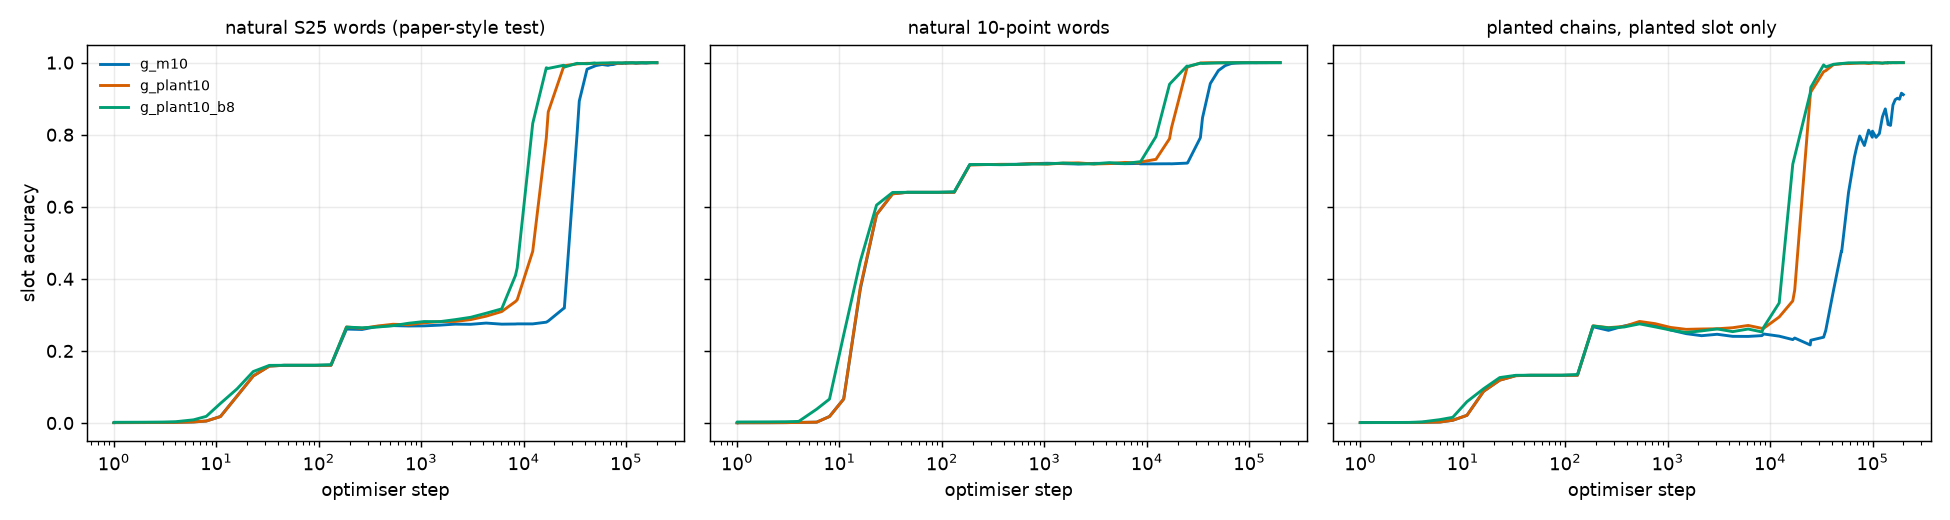
\includegraphics[width=1.00\linewidth]{fig_train_learning_curves.png}\caption{Accuracy (slot accuracy, teacher-forced) during training of the three general arms: natural 25-point words as in the paper’s test (left), natural 10-point words (middle) and the planted slot of planted chains of all tested $(L,s)$ cells (right). The $x$ axis is logarithmic.}\end{figure}

\lead{Learning curves.} Every arm goes through the same plateaus: first about 16\% (slot accuracy), then 27\%,
then a long stretch at 27–32\% on natural 25-point words, and then a rapid rise. The rise comes earlier for the
planted arms:

\begin{center}\small
\begin{tabular}{@{}l r >{\raggedright\arraybackslash}p{1.9cm} r >{\raggedright\arraybackslash}p{2.2cm}
>{\raggedright\arraybackslash}p{2.1cm} >{\raggedright\arraybackslash}p{2.1cm}@{}}
\toprule
\hdr{arm} & \hdr{blocks} & \hdr{steps (words)} & \hdr{wall time (h)} & \hdr{natural 25-point words, slots at least 90\% right} & \hdr{planted slots at least 90\% right} & \hdr{planted slots at least 99\% right} \\
\midrule
\code{g\_\allowbreak{}m10} & 5 & 200,000 (205M) & 5.33 & step 41,667 & step 175,000 & never \\
\code{g\_\allowbreak{}plant10} & 5 & 200,000 (205M) & 5.46 & step 24,676 & step 24,676 & step 41,667 \\
\code{g\_\allowbreak{}plant10\_\allowbreak{}b8} & 8 & 200,000 (205M) & 8.56 & step 16,667 & step 24,676 & step 33,333 \\
\code{e\_\allowbreak{}base} & 5 & 106,250 (109M), stopped by the deadline & 9.57 & step 45,833 (16-point uniform words) & step 106,250 & never \\
\bottomrule
\end{tabular}
\end{center}

So the planted chains bring the transition on natural words forward by 1.7 times (5 blocks) and 2.5 times (8
blocks), with one seed each; I do not know how much of that is seed-to-seed variation in the length of the
plateau. The control’s rise in planted accuracy is slower and not finished: 0.37 at step 41,667, 0.64 at 58,333,
0.81 at 100,000, 0.83 at 150,000 and 0.91 at 200,000, while its training loss on natural words falls from
$10^{-3}$ to $2\times10^{-5}$ over the same stretch. The learning rate also starts to decay at step 120,000, so
I cannot say whether the late gain is more data, the lower learning rate, or both.

Final accuracy on natural words (2,000 words per set, teacher-forced; for the elementary arm 2,000 words each):

\begin{center}\small
\begin{tabular}{@{}l >{\raggedright\arraybackslash}p{2.6cm} >{\raggedright\arraybackslash}p{2.8cm}
>{\raggedright\arraybackslash}p{4.2cm}@{}}
\toprule
\hdr{arm} & \hdr{10-point words: words right} & \hdr{25-point words: slots right} & \hdr{25-point words: words right} \\
\midrule
\code{g\_\allowbreak{}m10} & 100\% & 99.99\% & 99.75\% (1,995 of 2,000) \\
\code{g\_\allowbreak{}plant10} & 100\% & 99.95\% & 98.75\% (1,975 of 2,000) \\
\code{g\_\allowbreak{}plant10\_\allowbreak{}b8} & 100\% & 100\% & 100\% (2,000 of 2,000) \\
\code{e\_\allowbreak{}base} & training-like words: 99.4\% & 16-point uniform words: 99.6\% & 93.95\% \\
\bottomrule
\end{tabular}
\end{center}

(The last row has different test sets: words that look like the training data, and uniform words on the 16
points as in the paper’s real test file.) The original \code{torn-\allowbreak{}bigger-\allowbreak{}13} got
19,999 of 20,000 words on fresh natural words (\S\,\ref{sec:1} item 1); those are not the same words. It was
trained on 8M distinct words, each seen 161 times (about 1.3 billion words presented), where each general arm
here saw 205M distinct words once (table above). With one seed each, I would not read the small differences
between the three general arms as an effect of the data.

\begin{figure}[htbp]\centering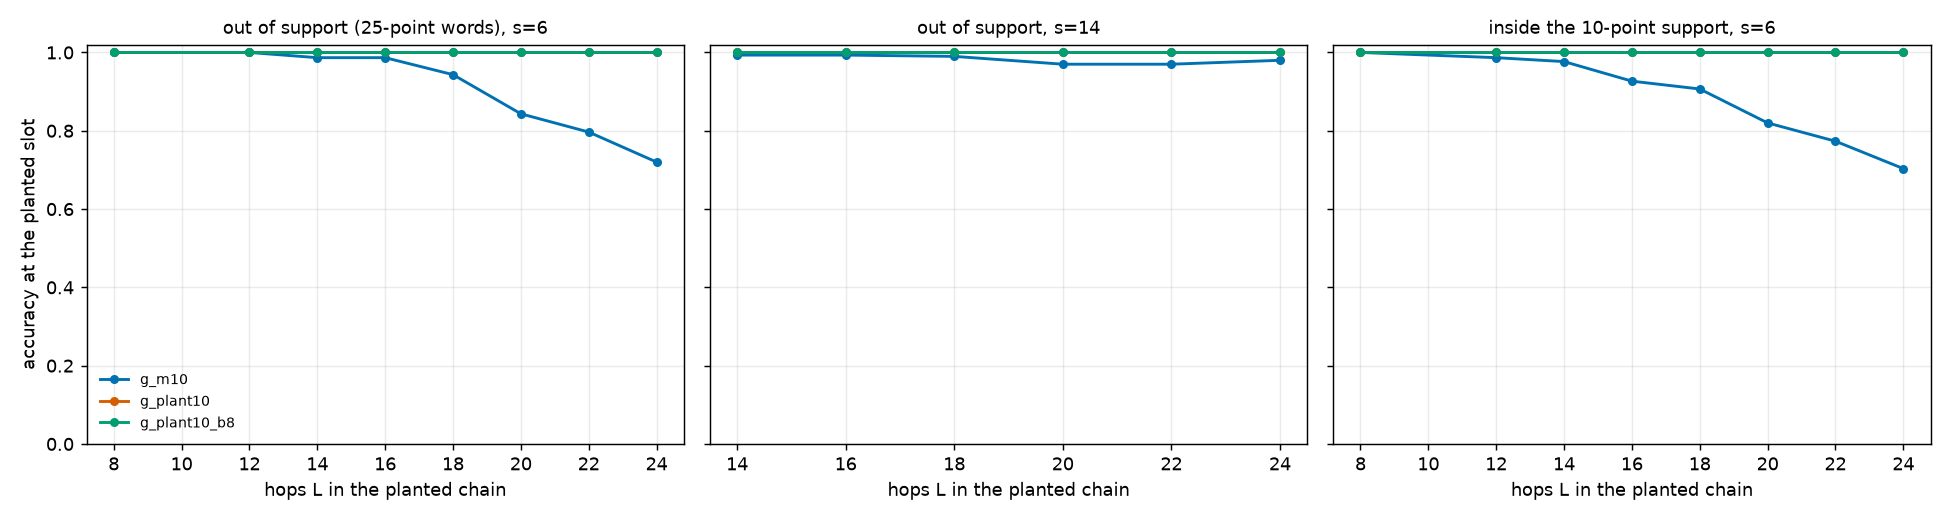
\includegraphics[width=1.00\linewidth]{fig_train_hop_cliff.png}\caption{Accuracy at the planted slot at the final checkpoint, by the number of hops $L$ in the planted chain, for chains through 6 points where the word is on 25 points (left), through 14 points (middle, outside the 10-point support) and through 6 points inside the 10-point support (right). \code{g\_\allowbreak{}plant10} (orange) is hidden behind \code{g\_\allowbreak{}plant10\_\allowbreak{}b8} (green): both are at 100\% at every point. 300 words per point.}\end{figure}

\lead{Planted chains at the final checkpoint} (300 words per cell; the planted slot only; $s$ is the number of
distinct points the chain visits, and every training word of the three general arms touches at most 10 points,
so $s\ge11$ is outside the support):

{\small\nopagebreak[4]
\begin{longtable}{@{}r r r r r@{}}
\toprule
\hdr{hops $L$} & \hdr{points $s$} & \hdr{\code{g\_\allowbreak{}m10} (\%)} & \hdr{\code{g\_\allowbreak{}plant10} (\%)} & \hdr{\code{g\_\allowbreak{}plant10\_\allowbreak{}b8} (\%)} \\
\midrule
\endfirsthead
\toprule
\hdr{hops $L$} & \hdr{points $s$} & \hdr{\code{g\_\allowbreak{}m10} (\%)} & \hdr{\code{g\_\allowbreak{}plant10} (\%)} & \hdr{\code{g\_\allowbreak{}plant10\_\allowbreak{}b8} (\%)} \\
\midrule
\endhead
\bottomrule
\endlastfoot
12 & 3 & 96.0 & 100 & 100 \\
12 & 6 & 100 & 100 & 100 \\
12 & 10 & 100 & 100 & 100 \\
16 & 3 & 73.7 & 100 & 100 \\
16 & 6 & 98.7 & 100 & 100 \\
16 & 10 & 99.0 & 100 & 100 \\
16 & 14 & 99.3 & 100 & 100 \\
20 & 3 & 64.7 & 100 & 100 \\
20 & 6 & 84.3 & 100 & 100 \\
20 & 10 & 97.7 & 100 & 100 \\
20 & 14 & 97.0 & 100 & 100 \\
20 & 20 & 98.3 & 100 & 100 \\
24 & 3 & 69.0 & 100 & 100 \\
24 & 6 & 72.0 & 100 & 100 \\
24 & 10 & 87.0 & 100 & 100 \\
24 & 14 & 98.0 & 100 & 100 \\
24 & 20 & 96.7 & 100 & 100 \\
\end{longtable}}

My own sweep (\code{run\_\allowbreak{}arm\_\allowbreak{}accuracy.\allowbreak{}py}, 300 words per cell,
$s=\min(L+1,10)$ and beyond the support up to $s=25$; summary in \code{summary.\allowbreak{}md}) agrees: 300 of
300 in all 19 cells for both planted arms, and for the control 100\% up to $L=12$, 98.3–99.3\% at $L=14$–20
($s=10$), 93.3\% at 22 and 88.3\% at 24 (my NumPy code gives 88\%, the training code 87\%).

\lead{The elementary arm} (\code{e\_\allowbreak{}base}, final checkpoint, step 106,250; my sweep
\code{run\_\allowbreak{}arm\_\allowbreak{}accuracy.\allowbreak{}py elem}, 300 words per cell). Planted chains
inside a window of 8 positions: 100\% up to 40 hops, 99.7\% at 56, 99.0\% at 70, 94.3\% at 80, 88.3\% at 100 and
85.3\% at 118 hops (the original model: 99.7\% at 80 and 94.7\% at 118, \S\,\ref{sec:3.13}). At 24 hops the
accuracy falls with the width of the window: 100\% at widths 4 and 8, 97.0\% at 11, 95.7\% at 12, 86.3\% at 14
and 66.7\% at 16 (the original: 95.6\% at width 16, \S\,\ref{sec:3.8}). So \code{e\_\allowbreak{}base} is less
accurate than the original elementary model, as expected from 1/14 of its word views, and the shapes agree: no
cliff in the number of hops, a fall with window width beyond about 12, and accuracy at 100 to 118 hops (82–88\%)
that is well above chance although my sample of its training data has no chain beyond about 78 hops.

\lead{How rare long chains are in the data.} In a natural word over 10 points, a pointer that sits on one of the
points is moved by each of the 25 letters independently with probability $0.18$ (the letter holds that point and
is not the identity: $2\times0.1\times0.9$), so the number of hops of a slot is exactly Binomial$(25, 0.18)$. I
checked this on 4M simulated slots (for example at least 12 hops: 2,335 observed against 2,313 expected; at
least 16: 2 against 1.9; the longest chain was 16). Each word has 10 such slots, so:

{\small\nopagebreak[4]
\begin{longtable}{@{}r >{\raggedright\arraybackslash}p{3.3cm} >{\raggedright\arraybackslash}p{4.2cm}
>{\raggedright\arraybackslash}p{4.2cm}@{}}
\toprule
\hdr{hops $L$} & \hdr{probability per slot of at least $L$ hops} & \hdr{expected slots in the control’s 205M words (2.05 billion slots)} & \hdr{expected slots in the original 8M-word file (80M slots)} \\
\midrule
\endfirsthead
\toprule
\hdr{hops $L$} & \hdr{probability per slot of at least $L$ hops} & \hdr{expected slots in the control’s 205M words (2.05 billion slots)} & \hdr{expected slots in the original 8M-word file (80M slots)} \\
\midrule
\endhead
\bottomrule
\endlastfoot
12 & $5.8\times10^{-4}$ & 1,200,000 & 46,000 \\
14 & $2.2\times10^{-5}$ & 46,000 & 1,800 \\
16 & $4.7\times10^{-7}$ & 960 & 38 \\
18 & $5.1\times10^{-9}$ & 10 & 0.4 \\
20 & $2.7\times10^{-11}$ & 0.05 & 0.002 \\
22 & $5.4\times10^{-14}$ & 0.0001 & $4\times10^{-6}$ \\
24 & $2.8\times10^{-17}$ & $6\times10^{-8}$ & $2\times10^{-9}$ \\
\end{longtable}}

So the control saw about 10 slots of 18 hops or more in the whole run, and (in expectation) none of 20 or more,
and still gets 97.7\% at $L=20$ with $s=10$. It generalises about two to four hops beyond where its training
chains run out. Of the possible words: a 25-letter word has 625 possible letters per position, so there are
$625^{25}\approx10^{69.9}$ words, and 205M is $2.6\times10^{-62}$ of them; natural words over 10 points number
about $100^{25}\binom{25}{10}\approx3\times10^{56}$ (an overestimate, because words that use fewer than 10
points are counted several times), so the expected number of repeated words among 205M fresh ones is about
$6\times10^{-41}$: none.

\begin{center}\small
\begin{tabular}{@{}>{\raggedright\arraybackslash}p{6.0cm} >{\raggedright\arraybackslash}p{8.6cm}@{}}
\toprule
\hdr{prediction written before the run (\S\,\ref{sec:6.1})} & \hdr{outcome} \\
\midrule
Coverage: \code{g\_\allowbreak{}plant10} at 90\% or more at 20 to 24 hops at every $s$, including $s=14$ and 20 & \textbf{Confirmed.} 100\% in all 17 cells above and in all 19 of my sweep, including $s=14$ to 25 \\
Depth: \code{g\_\allowbreak{}plant10} still falls off between about 16 and 24 hops, and \code{g\_\allowbreak{}plant10\_\allowbreak{}b8} does not & \textbf{Refuted for \code{g\_\allowbreak{}plant10}.} The five-block planted model does not fall off at all, so the eight-block model has nothing to improve on (a ceiling) \\
The control reproduces the cliff at 15 to 20 hops & \textbf{Not reproduced.} 97–100\% at $L=14$ to 20 with $s\ge10$; the original model was at about 51\% at $L=20$ \\
Mixed outcomes are plausible & The control is worse than the planted arms at $L\ge22$ and for chains through few points; it does not show a cliff \\
\code{e\_\allowbreak{}base}: no prediction & See the paragraph above and \S\,\ref{sec:3.15} \\
\bottomrule
\end{tabular}
\end{center}

\begin{findbox}{What this does and does not say}
\begin{itemize}
\item \lead{Five blocks are enough for 24 hops when the data contains such chains.}
  \code{g\_\allowbreak{}plant10} has 100\% at 24 hops through 3 to 20 points with 5 blocks and 6 heads. A reach
  that doubles with each block would cap five blocks at about 16 hops (the reading of \S\,\ref{sec:3.9}), so
  this model either grows its reach faster than doubling or composes chains in another way. \S\,\ref{sec:3.16}
  shows that its probes do not follow the staircase, and I did not find the mechanism. This refutes a limit of
  the architecture, not one of the rule \code{torn-\allowbreak{}bigger-\allowbreak{}13} learned:
  \S\,\ref{sec:3.17} finds that the original’s accuracy on fresh chains falls with the number of hops whatever
  the number of points.
\item \lead{The data do matter at the edges.} The control is at 97–99\% for $L\le20$ with 10 or more points, but
  falls to 87\% at $L=24$ with 10 points and to 65–74\% for chains through 3 points at $L\ge16$, which natural
  words essentially never contain (for a slot that has 16 hops, the chance that they visit only 3 points is
  about $4\times10^{-9}$). Adding planted chains removes all of these. This is a difference in coverage of the
  pair $(L,s)$, not of $L$ alone, which is a refinement of \S\,\ref{sec:3.3}: for the original model I found $s$
  almost irrelevant at $L=20$ (about 50–56\% at 4 or at 21 points); for the control, the weak spot is chains
  with few points.
\item \lead{The original model’s cliff is not reproduced, and I do not know why.} The control matches the data
  distribution of \code{torn-\allowbreak{}bigger-\allowbreak{}13} but differs from the original run in at least:
  fresh data at every step (205M distinct words, each seen once) instead of an 8M-word file read 161 times, a
  batch of 1,024 words instead of 4,096 and 200,000 steps instead of about 315,000, my own learning-rate
  schedule, fused attention without DeepSpeed, and one seed (the original run also used bfloat16, so that is not
  a difference; version 9 listed it as one). These pull in different directions: the control saw 25 times as
  many distinct words, and so many more chains of every length, and about a sixth as many words presented, so
  fewer updates. A cliff that came from repeating a finite file would be absent from the control for the first
  reason; I did not test that (\S\,\ref{sec:6}, priority 2). The result says that the cliff is not a property of
  five blocks together with natural words over 10 points as such; it does not say which of these differences
  made the original’s cliff.
\item \lead{The eight-block arm answers nothing about depth}, because the five-block planted arm is already at
  the ceiling of the test. A depth test needs a model with fewer blocks (the 3-block arm listed in
  \S\,\ref{sec:6.1}) or a harder task.
\item Not tested: more than one seed, a control trained longer or with a constant learning rate, and chains
  longer than 24 hops (a 25-letter word cannot hold them).
\end{itemize}
\end{findbox}

\begin{limbox}{Limits}
One seed per arm; the planted test words are drawn by the same generator as half of the planted arms’ training
data (so “100\%” is in-distribution for them at $s\le10$, and outside it for $s\ge11$);
\code{e\_\allowbreak{}base} was stopped at 97\% of its steps; 300 words per cell; the tests are teacher-forced
at the planted slot.
\end{limbox}

\subsection{Position embeddings of the elementary arm during training: has the block at 72 formed?
(\texorpdfstring{\code{e\_\allowbreak{}base}}{e_base})}\label{sec:3.15}
\lead{Why.} In the original elementary model (Figure 5b, \S\,\ref{sec:3.8}) the word-position embeddings split
into two blocks at position 72, and the 16 output positions form a third at 120. The training data are
position-stationary (\S\,\ref{sec:3.8}), so the block is learned and not read off the data. The question for the
run was when, if at all, such blocks appear in \code{e\_\allowbreak{}base}.

\lead{What I measured} (\code{make\_\allowbreak{}ebase\_\allowbreak{}figure.\allowbreak{}py}; the position
embeddings of \code{e\_\allowbreak{}base} at 59 snapshots are in the run’s
\code{pos\_\allowbreak{}emb.\allowbreak{}npz}, and the original is the checkpoint of \S\,\ref{sec:3.8}). For
each snapshot, the cosine between the embeddings of positions $t$ and $t+1$ for $t=0,\dots,118$: the median over
$t$, the value at $t=71$ (the pair across the boundary at 72) and the smallest value. I also repeated the
comparison of rows used in \code{fig5b\_\allowbreak{}provenance.\allowbreak{}py} (how much row $k$ and row $k+1$
of the cosine matrix differ outside the diagonal band, for $k$ from 61 to 119), which is what finds the boundary
at 72 in the original.

\begin{figure}[htbp]\centering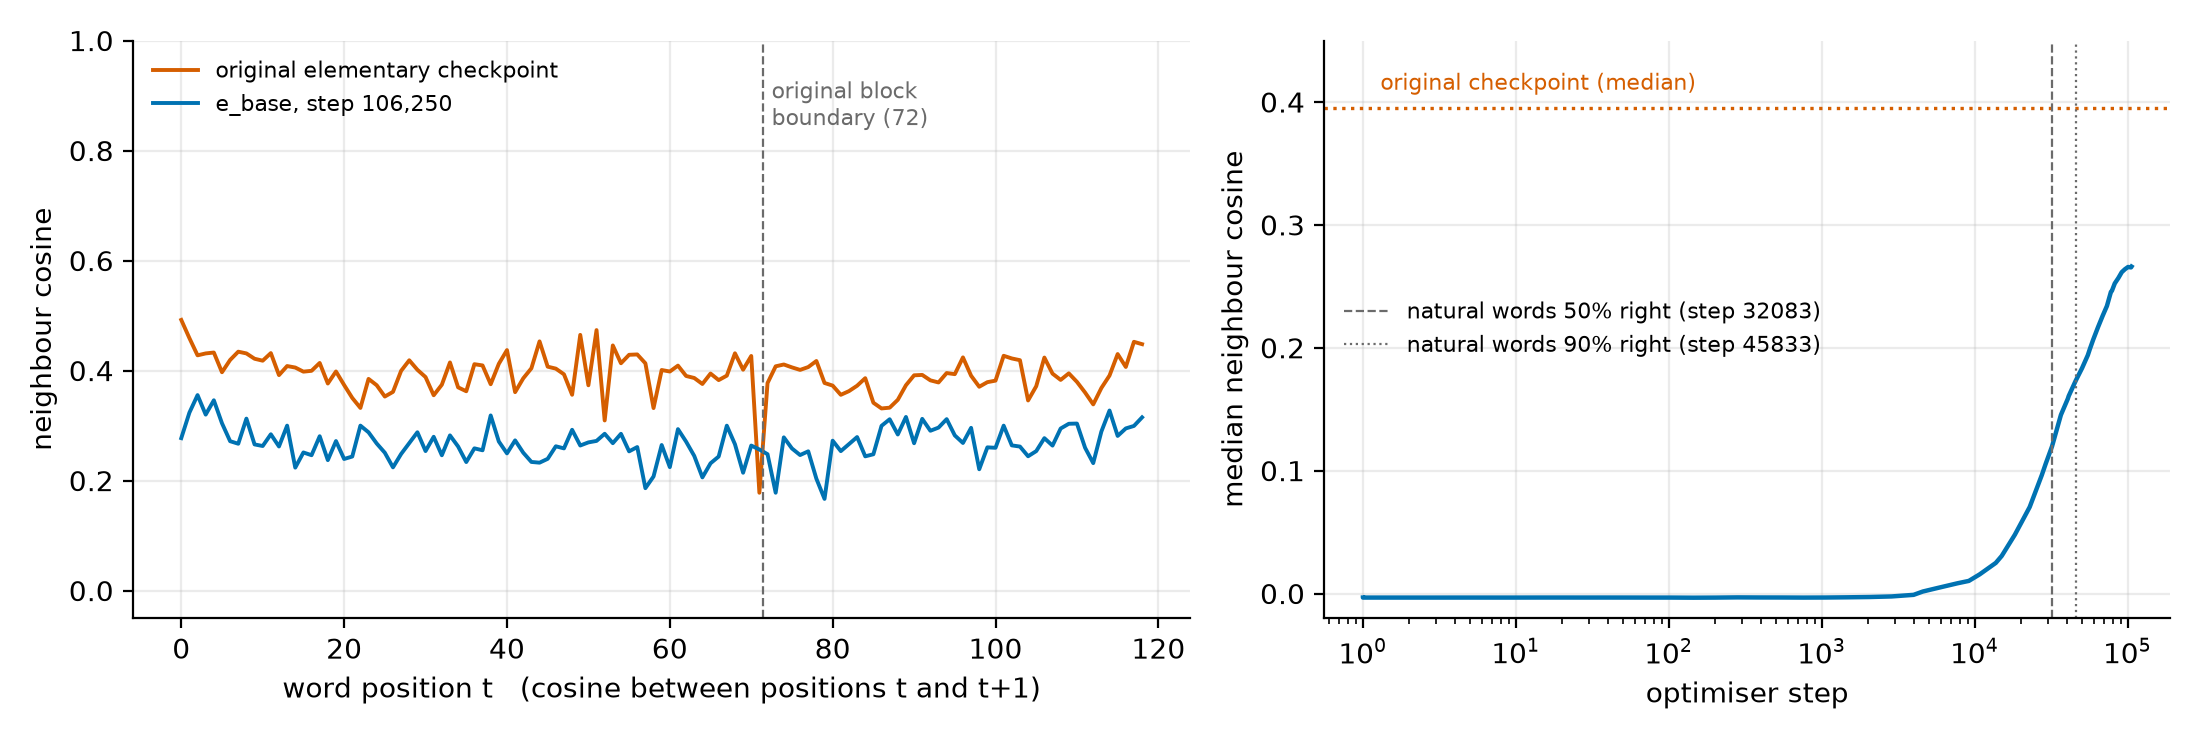
\includegraphics[width=1.00\linewidth]{fig_ebase_blocks.png}\caption{Left: cosine between the embeddings of word positions $t$ and $t+1$, for the original elementary checkpoint (orange) and \code{e\_\allowbreak{}base} at its final step (blue). Right: the median of that quantity over $t$ during training of \code{e\_\allowbreak{}base}, with the steps at which natural words reach 50\% and 90\% slot accuracy.}\end{figure}

\begin{center}\small
\begin{tabular}{@{}>{\raggedright\arraybackslash}p{5.0cm} >{\raggedright\arraybackslash}p{4.0cm}
>{\raggedright\arraybackslash}p{4.6cm}@{}}
\toprule
\hdr{} & \hdr{original checkpoint} & \hdr{\code{e\_\allowbreak{}base}, step 106,250} \\
\midrule
median neighbour cosine & 0.40 & 0.27 \\
value across the boundary, $t=71$ & \textbf{0.18} (the smallest of all 119 pairs) & 0.26 (median 0.27) \\
smallest value, and where & 0.18 at $t=71$ & 0.17 at $t=79$ \\
\bottomrule
\end{tabular}
\end{center}

The median neighbour cosine of \code{e\_\allowbreak{}base} is about 0 up to step 4,000 (random initialisation),
then grows: 0.01 at step 7,746, 0.03 at 15,037, 0.10 at 27,500, 0.16 at 40,670, 0.19 at 55,000, 0.23 at 68,750,
0.25 at 82,500 and 0.27 at the end.

\begin{findbox}{What it shows}
\begin{itemize}
\item \lead{There is no block at 72 in \code{e\_\allowbreak{}base} yet.} The pair $(71,72)$ is as similar as a
  typical neighbour pair (0.26 against a median of 0.27), where the original has its lowest value (0.18 against
  0.40). The row comparison does not single out 72 either: its largest values are at 79 and 82.
\item \lead{The positions become smooth first, from the diagonal outwards, and this starts before the accuracy
  jump.} The neighbour cosine is already 0.03 at step 15,037 and 0.10 at 27,500, before natural words reach 50\%
  slot accuracy (step 32,083) and 90\% (step 45,833); it keeps growing afterwards and is still rising at the
  end. The position-embedding pictures in
  \code{figures/\allowbreak{}pos\_\allowbreak{}pictures\_\allowbreak{}e\_\allowbreak{}base.\allowbreak{}png} of
  the run show this as a band along the diagonal that widens and gets structure at steps 41,250 to 106,250, and
  a faint separate square for the 16 output positions in the corner.
\item \lead{The lowest neighbour cosine moves around}: at $t=60$ from initialisation to about step 15,000, at 73
  from step 27,500 to 68,750 and at 79 from step 82,500. Position 79 is already among the two largest row
  differences at initialisation (with 64), so at least that dip may come from the random initialisation and not
  from the data; I did not test this with a second seed.
\item \lead{So the block is not an early event of training in this run.} \code{e\_\allowbreak{}base} has seen
  109M distinct words, each once; the original elementary model was trained on 16M distinct words for 96 epochs,
  about 1.5 billion words presented, and has a median neighbour cosine that \code{e\_\allowbreak{}base} has not
  reached. So \code{e\_\allowbreak{}base} has had one fourteenth of the original’s words presented and about 7
  times its distinct words, and I cannot say which of the two matters for the block; I tested neither. Whether a
  block at 72 (or somewhere) appears with much longer training, with a repeated finite file, with another seed,
  or never, I cannot say from this run. \S\,\ref{sec:3.18}: in the Spartan model folder a boundary appears in
  about half the fully trained runs with this config, at 72 to 81, whatever their length of training.
\end{itemize}
\end{findbox}

\begin{limbox}{Limits}
One seed, one arm, stopped at 97\% of its planned steps, and the cosine of neighbours is a crude summary of the
block structure (the original’s block is found from the whole matrix, which I only compared by rows).
\end{limbox}

\subsection{Inside the retrained models: probes, attention, ablation and patching (Tests 7 to 12 on the new
checkpoints, and Test 15)}\label{sec:3.16}
\lead{What was run.} The tests of \S\,\ref{sec:3.9} to \S\,\ref{sec:3.12}, unchanged, on the final checkpoint of
each arm (\code{analyze\_\allowbreak{}run.\allowbreak{}py}; per-arm result files and logs are in
\code{analysis-\allowbreak{}20261126-\allowbreak{}121524/\allowbreak{}<arm>/}; side-by-side tables in
\code{analysis-\allowbreak{}20261126-\allowbreak{}121524/\allowbreak{}summary.\allowbreak{}md}). The scripts
take the checkpoint from environment variables (\code{ckpt\_\allowbreak{}env.\allowbreak{}py}), so the same code
runs on the original and on the new models. The 8-block model was checked by running a padded copy of the
5-block original through the pipeline: the results agree exactly on the shared blocks. The probes and the
attention analysis use the same planted and natural words as before. A new test, Test 15 (greedy ablation), is
described below. Every number is for one checkpoint of one seed.

\lead{Probes at the word positions (Test 7).} Accuracy (\%) of the continuation probe of \S\,\ref{sec:3.9}
(chance 4\%) at the last two layers that matter, by the number of hops $h$ still to go. The last layer of each
model is shown for completeness: no block reads the word positions after it, so what is computed there is not
used.

{\small\nopagebreak[4]
\begin{longtable}{@{}l *{8}{r}@{}}
\toprule
\hdr{model, layer} & \hdr{$h=1$} & \hdr{2} & \hdr{3} & \hdr{4} & \hdr{5–6} & \hdr{7–8} & \hdr{9–12} & \hdr{13–24} \\
\midrule
\endfirsthead
\toprule
\hdr{model, layer} & \hdr{$h=1$} & \hdr{2} & \hdr{3} & \hdr{4} & \hdr{5–6} & \hdr{7–8} & \hdr{9–12} & \hdr{13–24} \\
\midrule
\endhead
\bottomrule
\endlastfoot
original \code{torn-\allowbreak{}bigger-\allowbreak{}13}, layer 4 & 77 & 66 & 61 & 60 & 47 & 40 & 10 & 5 \\
original, layer 5 & 75 & 64 & 61 & 64 & 56 & 57 & 64 & 74 \\
\code{g\_\allowbreak{}m10}, layer 4 & 76 & 53 & 46 & 41 & 38 & 4 & 4 & 6 \\
\code{g\_\allowbreak{}m10}, layer 5 & 75 & 52 & 49 & 43 & 46 & 49 & 49 & 53 \\
\code{g\_\allowbreak{}plant10}, layer 4 & 65 & 50 & 46 & 30 & 6 & 4 & 7 & 6 \\
\code{g\_\allowbreak{}plant10}, layer 5 & 63 & 50 & 47 & 32 & 14 & 17 & 26 & 38 \\
\code{g\_\allowbreak{}plant10\_\allowbreak{}b8}, layer 7 & 79 & 57 & 45 & 35 & 17 & 20 & 28 & 29 \\
\code{g\_\allowbreak{}plant10\_\allowbreak{}b8}, layer 8 & 78 & 55 & 45 & 39 & 45 & 54 & 61 & 69 \\
\end{longtable}}

\begin{findbox}{What it shows}
\begin{itemize}
\item \lead{The staircase is later and flatter in the retrained models than in the original.} At layer 4 the
  control’s probe reads $h=1$ and 2 at 76\% and 53\%, $h=3$ to 6 at 38–46\% and nothing beyond (4–6\%), where
  the original reads $h\le4$ at 60–77\% and $h=5$ to 8 at 40–47\%; everything beyond 6 hops appears only at the
  last layer, at about 50\%. So the staircase of \S\,\ref{sec:3.9} (about 1, 1, 4, 8 and 13 or more hops at
  layers 1 to 5) is not a fixed property of this architecture and data distribution: the control has the
  original’s architecture and data distribution and a shorter reach at layer 4.
\item \lead{\code{g\_\allowbreak{}plant10} answers 24 hops with probes that read less.} At layer 5, where the
  original reads 56–74\% at every $h$ and the control about 50\%, it reads 14–38\% at $h\ge5$, although it is
  right on 100\% of the planted chains. The linear probe does not read what this model uses, and I cannot say
  what that is.
\item \lead{More blocks do not bring the reach earlier.} In the 8-block model, $h=1$ is readable from layer 5,
  $h=2$ from layer 6, $h=3$ from layer 7 (45\%), and every $h$ only at layer 8 (45–78\%). The three extra blocks
  have pushed the staircase back by three layers; they have not given it a bigger step.
\item \code{e\_\allowbreak{}base} has the staircase of the original elementary model: at layer 4 its probe reads
  $h\le4$ at 62–93\%, $h=5$ to 6 at 47\% and $h=7$ to 8 at 42\%, against 66–89\%, 50\% and 45\% for the original
  (\S\,\ref{sec:3.11}), and 31\% against 23\% at $h=9$ to 12.
\end{itemize}
\end{findbox}

\lead{Attention (Test 11).} The strongest hop offsets of the heads at the word positions, at the longest $L$
tested: in \code{g\_\allowbreak{}m10} ($L=16$), $\pm1$ only (11 to 13 times uniform attention), in blocks 2 and
3; in \code{g\_\allowbreak{}plant10} ($L=24$), $\pm1$ in blocks 2 and 3 (9 to 13 times) and one head at $+2$
(block 3 head 4, 9 times); in \code{g\_\allowbreak{}plant10\_\allowbreak{}b8} ($L=24$), $\pm1$ in blocks 2 to 6
(9 to 10 times). None of them has offsets that grow with depth, so there is no doubling in the attention of the
general models, which agrees with the original general model (\S\,\ref{sec:3.12}), and does not explain how 24
hops are composed. \code{e\_\allowbreak{}base} shows the doubling of the original elementary model (at $L=80$):
offsets $\pm1$ (up to 66 times uniform), with some $\pm2$ and $\pm3$ (10 to 32 times) in blocks 1 and 2, $\pm1$
to $\pm4$ in block 3 (up to 42 times) and $\pm4$ to $\pm8$ in block 4 (8 to 10 times).

\lead{Single-head ablation (Test 12).} Zeroing one head at the word positions (blocks 1 to $n-1$; block $n$ is
never read there), compared with replacing it by its mean over 150 other words:

\begin{center}\small
\begin{tabular}{@{}>{\raggedright\arraybackslash}p{2.9cm} >{\raggedright\arraybackslash}p{3.2cm}
>{\raggedright\arraybackslash}p{8.0cm}@{}}
\toprule
\hdr{arm, $L$} & \hdr{heads that cost more than 10 points} & \hdr{the three costliest, accuracy with the head zeroed (mean replacement)} \\
\midrule
\code{g\_\allowbreak{}m10}, 16 & 6 of 24 & b1h2: 0.37 (0.37); b3h5: 0.46 (0.58); b2h3: 0.48 (0.82) \\
\code{g\_\allowbreak{}plant10}, 24 & 4 of 24 & b2h1: 0.46 (0.98); b2h3: 0.61 (0.99); b2h4: 0.64 (0.99) \\
\code{g\_\allowbreak{}plant10\_\allowbreak{}b8}, 24 & 2 of 42 & b2h5: 0.69 (0.94); b2h3: 0.86 (0.97); b6h2: 0.91 (0.94) \\
\code{e\_\allowbreak{}base}, 80 & 17 of 24 & b1h5: 0.39 (0.47); b2h3: 0.43 (0.43); b1h4: 0.45 (0.42) \\
\bottomrule
\end{tabular}
\end{center}

\begin{findbox}{What it shows}
In the planted arms no single head matters much: the costliest ones lose 9 to 54 points when zeroed and at most
6 when replaced by their mean, so what these heads give is a word-independent contribution that the later blocks
expect, not information about the word that no other head provides. In the control, the heads b1h2 and b3h5 do
carry word-dependent information that nothing replaces (their mean replacement is as bad as zeroing or nearly).
\code{e\_\allowbreak{}base} is the opposite case: 17 of its 24 heads cost more than 10 points at 80 hops and
mean replacement is about as bad as zeroing, so it uses many heads, each of which carries word-dependent
information.
\end{findbox}

\lead{Greedy ablation (Test 15; \code{run\_\allowbreak{}greedy\_\allowbreak{}ablation.\allowbreak{}py}).} Single
heads cannot show redundancy (\S\,\ref{sec:3.13}). Starting from no head removed, I zeroed at each step the one
further head at the word positions whose removal lowered the accuracy at the planted slot the most, on planted
words of the longest $L$ tested that the intact model answers correctly (150 words), for at most 8 heads, and
stopped below 15\%.

\begin{center}\small
\begin{tabular}{@{}>{\raggedright\arraybackslash}p{2.6cm} r r >{\raggedright\arraybackslash}p{9.0cm}@{}}
\toprule
\hdr{arm} & \hdr{$L$} & \hdr{words} & \hdr{heads removed in this order (accuracy after each removal; 1.00 with none removed)} \\
\midrule
\code{g\_\allowbreak{}m10} & 16 & 149 & b3h5 (0.43), b1h2 (0.30), b2h3 (0.18), b1h4 (0.17), b3h4 (0.15), b2h2 (0.15) \\
\code{g\_\allowbreak{}plant10} & 24 & 150 & b2h1 (0.51), b2h5 (0.39), b2h3 (0.31), b2h2 (0.25), b3h3 (0.20), b1h0 (0.19), b1h4 (0.20), b1h5 (0.21) \\
\code{g\_\allowbreak{}plant10\_\allowbreak{}b8} & 24 & 150 & b2h5 (0.75), b2h3 (0.38), b1h3 (0.29), b5h3 (0.24), b2h1 (0.23), b1h0 (0.23), b1h1 (0.23), b1h2 (0.23) \\
\code{e\_\allowbreak{}base} & 80 & 146 & b1h5 (0.33), b3h1 (0.32), b2h3 (0.31), b2h1 (0.28), b4h0 (0.27), b1h3 (0.25), b2h2 (0.24), b3h2 (0.25) \\
\bottomrule
\end{tabular}
\end{center}

\begin{findbox}{What it shows}
\begin{itemize}
\item \lead{Removing three to five heads of 24 takes every general model to 15–31\% at the longest $L$ tested.}
  Removing three heads brings the accuracy at the planted slot from 1.00 to 0.18 in the control ($L=16$; b3h5,
  b1h2, b2h3), to 0.31 in \code{g\_\allowbreak{}plant10} (b2h1, b2h5, b2h3) and to 0.29 in
  \code{g\_\allowbreak{}plant10\_\allowbreak{}b8} (b2h5, b2h3, b1h3, out of 42). The control reaches 15\% with
  five heads and my stopping rule (below 15\%) ends the search at six (0.148). The two planted models do not go
  below 0.19 (\code{g\_\allowbreak{}plant10}, six heads) and 0.23
  (\code{g\_\allowbreak{}plant10\_\allowbreak{}b8}, from five heads on) within 8 heads: their accuracy drops
  steeply over the first three or four heads and then flattens at a level well above chance (0.04), which I did
  not look into.
\item \lead{The first heads removed are in blocks 1 to 3,} mostly block 2 (all of the first three in
  \code{g\_\allowbreak{}plant10}, two of three in \code{g\_\allowbreak{}plant10\_\allowbreak{}b8}, one each in
  blocks 1, 2 and 3 in the control); the fourth in the 8-block model is in block 5 (b5h3). In
  \code{g\_\allowbreak{}plant10} and \code{g\_\allowbreak{}plant10\_\allowbreak{}b8} the same two heads, b2h5
  and b2h3, are among the first three. \code{g\_\allowbreak{}m10} and \code{g\_\allowbreak{}plant10} started
  from the same random weights (\S\,\ref{sec:6.1}), and I did not check whether the first blocks of
  \code{g\_\allowbreak{}plant10\_\allowbreak{}b8} did too, so I do not read the coincidence as an independent
  finding. In \code{torn-\allowbreak{}bigger-\allowbreak{}13} these two heads are the next-hop head b2h5 and the
  previous-hop head b2h3 (\S\,\ref{sec:3.13}).
\item \lead{This is redundancy of a particular kind.} In the planted models a single head is cheap to replace by
  its mean (at most 6 points, \S\,\ref{sec:3.16}), yet three of them zeroed together leave 30\% of the answers.
  So the model needs these heads to be present and to give a typical output, not to give a word-specific one.
  The greedy set is not shown to be the mechanism: zeroing puts the later blocks into states they never see, so
  a collapse after zeroing a few heads is an upper bound on what these heads do, and a test with mean
  replacement of the whole set would be a better measure. I did not run it.
\item \lead{\code{e\_\allowbreak{}base} is different in shape.} At 80 hops one head, b1h5, takes it from 1.00 to
  0.33, the next seven cost only 8 more points (0.25 after eight heads, never below 0.15), where chance is 0.06.
  This agrees with \S\,\ref{sec:3.16}, where 17 of its 24 heads cost more than 10 points on their own: nearly
  every head matters, and the first removal already takes away two thirds of the correct answers. After that
  there is little left to remove at 80 hops that the greedy order can find, and I did not look into what the
  model answers at that floor.
\end{itemize}
\end{findbox}

\lead{Activation patching (Test 8 re-run).} The tests of \S\,\ref{sec:3.10}: corrupt one hop letter, patch clean
activations back into the corrupted run, at $L=8$, 12 and 16, 200 words per condition (the models are right on
the clean words).

\begin{itemize}
\item \lead{For a middle or last hop, the last readable block reads the answer from the word positions in every
  retrained model, as in the original.} Patching all word positions after block $n-1$ restores 1.00 of the words
  in \code{g\_\allowbreak{}plant10} and \code{g\_\allowbreak{}plant10\_\allowbreak{}b8} at every $L$, and 0.98
  to 1.00 in the control (0.99 at $L=16$, last hop). Patching only the letters to the right of the corrupted
  middle hop at the same layer restores 0.78 in the control (original 0.92), 0.45 in
  \code{g\_\allowbreak{}plant10} and 0.45 in \code{g\_\allowbreak{}plant10\_\allowbreak{}b8} ($L=12$), while
  patching the chain letters restores 0.98 to 1.00 in all. Patching the letters to the left of the corrupted hop
  (read later) restores 0.17 and 0.20 in the two planted arms and 0.06 in the control, so in the planted arms
  the information about a hop letter is a little more spread over the chain and less concentrated on the letters
  read before it.
\item \lead{The first hop is read by the query earlier in the control and later in the planted arms.} Share
  restored at $L=12$ when the first hop is corrupted and all word positions are patched after block $\ell$:
\end{itemize}

{\small\nopagebreak[4]
\begin{longtable}{@{}r r r r r@{}}
\toprule
\hdr{$\ell$} & \hdr{original} & \hdr{\code{g\_\allowbreak{}m10}} & \hdr{\code{g\_\allowbreak{}plant10}} & \hdr{\code{g\_\allowbreak{}plant10\_\allowbreak{}b8}} \\
\midrule
\endfirsthead
\toprule
\hdr{$\ell$} & \hdr{original} & \hdr{\code{g\_\allowbreak{}m10}} & \hdr{\code{g\_\allowbreak{}plant10}} & \hdr{\code{g\_\allowbreak{}plant10\_\allowbreak{}b8}} \\
\midrule
\endhead
\bottomrule
\endlastfoot
0 & 1.00 & 1.00 & 1.00 & 1.00 \\
1 & 1.00 & 1.00 & 1.00 & 1.00 \\
2 & 0.43 & 0.47 & 0.90 & 1.00 \\
3 & 0.10 & 0.07 & 0.48 & 0.41 \\
4 & 0.04 & 0.05 & 0.21 & 0.24 \\
5 &  & 0.05 & 0.04 & 0.23 \\
6 &  &  &  & 0.07 \\
7 &  &  &  & 0.03 \\
8 &  &  &  & 0.03 \\
\end{longtable}}

A high value means that the query has not yet taken in the corrupted first hop at that layer. In the control the
query has taken it in by block 3, as in the original. In \code{g\_\allowbreak{}plant10} it has hardly taken it
in by block 2 (0.90) and does so over blocks 3 and 4; in the 8-block model it has not taken it in by block 2
either (1.00) and does so over blocks 3 to 6.

\begin{itemize}
\item \lead{\code{e\_\allowbreak{}base} agrees with the original elementary model for a middle or last hop, and
  takes in the first hop earlier} (\code{run\_\allowbreak{}patching\_\allowbreak{}elem.\allowbreak{}py}, $L=12$,
  24, 40 and 80, about 200 words per $L$, results in
  \code{e\_\allowbreak{}base/\allowbreak{}patching\_\allowbreak{}elem\_\allowbreak{}results\_\allowbreak{}e\_\allowbreak{}base.\allowbreak{}json}).
  Restoring all word positions after block 4 brings back the clean answer in 1.00 of the words for a corrupted
  middle or last hop at every $L$, as in \S\,\ref{sec:3.11}, and the letters to the right of a corrupted last
  hop restore it from block 3 on (0.94–1.00 after block 4, against 1.00 for the original at $L=40$). For the
  first hop the original is still repairable after block 3 (0.97–1.00 at every $L$) and not after block 4
  (0.02–0.17). In \code{e\_\allowbreak{}base} the share restored after blocks 2, 3 and 4 is 0.72, 0.37 and 0.07
  at $L=12$; 0.54, 0.19 and 0.06 at $L=24$; 0.39, 0.14 and 0.07 at $L=40$; and 0.47, 0.26 and 0.22 at $L=80$
  (0.22 is the share of words that are right without any patch). So its query position has taken in the first
  hop about one block earlier than the original’s, which may be a difference of training length or of seed.
\end{itemize}

\begin{findbox}{What this does and does not say}
\begin{itemize}
\item \lead{The planted models differ from the original and from the control in every internal measurement I
  made} (one seed each; these are differences in measurements, not a demonstrated difference in algorithm), with
  less probe-readable structure at the word positions, little reliance on any single head, a collapse when 4 or
  5 of the 24 word-position heads are removed together, and a later hand-over of the first hop to the query. I
  did not find the mechanism, and the hop offsets of attention do not show doubling in any of the general
  models.
\item \lead{The extra blocks of the 8-block model are used for the same pattern, later}: the probe staircase and
  the first-hop patching are pushed back by about three layers, not made steeper.
\item \code{e\_\allowbreak{}base} reproduces what I found in the original elementary model (the probe staircase,
  the doubling of hop offsets with depth, patching) at 97\% of its planned training, with many heads each
  needed.
\end{itemize}
\end{findbox}

\begin{limbox}{Limits}
One checkpoint per arm; probes are linear and trained within the arm; attention is not causal; zeroing is a
blunt tool; the greedy order is greedy and not the best possible subset; patching is at the word positions all
at once, not one head at a time.
\end{limbox}

\subsection{Memorisation, and hops against points (Test 16)}\label{sec:3.17}
\lead{Why.} The wandb history of \code{torn-\allowbreak{}bigger-\allowbreak{}13} (exported by you on 27 Nov
2026) shows the run trained for 161 epochs on 12 Feb 2025 and, nine months later, for 24 more epochs after an
automatic resume with a fresh optimiser (\S\,\ref{sec:3.18}). Its training loss and its validation loss agree
within a factor of 1 to 2 until about epoch 80; between epochs 81 and 100 the training loss falls to about
$4\times10^{-9}$ while the validation loss stays near $10^{-5}$, a ratio of 2,000 to 3,800 from then on. The
learning rate is not logged; replaying \code{ReduceLROnPlateau} on the logged training loss puts its drops
either at epochs 86, 119, 130, 141 and 152 or at 4, 61, 69, 73 and 77 (if accelerate stepped the scheduler once
per process), down to $3\times10^{-9}$ either way, and the resume favours the second reading. The question: does
the model know the long chains of its own training file better than fresh ones?

\lead{Test 16} (\code{run\_\allowbreak{}memorisation.\allowbreak{}py}). Every output slot of all 8M training
words (commit \code{5863de5}, the run’s data) gets its hop count $h$. Training slots with $h\ge12$ (up to 1,500
per $h$, and all with $h\ge14$), slots of the run’s validation file, and fresh natural slots found by rejection
among 60M generated words (the generator matches the file: at least 12 hops in $2.31\times10^{-4}$ of training
slots and $2.30\times10^{-4}$ of generated ones). Teacher-forced accuracy and median margin at the slot. The
same slots then go through the resumed model, the fresh-data control and \code{g\_\allowbreak{}plant10}; for
those, the training slots of \code{torn-\allowbreak{}bigger-\allowbreak{}13} are just more held-out words.

{\small\nopagebreak[4]
\begin{longtable}{@{}r r >{\raggedright\arraybackslash}p{2.0cm} >{\raggedright\arraybackslash}p{2.0cm}
>{\raggedright\arraybackslash}p{2.0cm} >{\raggedright\arraybackslash}p{2.0cm}
>{\raggedright\arraybackslash}p{2.0cm}@{}}
\toprule
\hdr{hops $h$} & \hdr{training slots} & \hdr{Feb 2025, its training slots} & \hdr{Feb 2025, fresh} & \hdr{resumed, fresh} & \hdr{\code{g\_\allowbreak{}m10}, fresh} & \hdr{\code{g\_\allowbreak{}plant10}, fresh} \\
\midrule
\endfirsthead
\toprule
\hdr{hops $h$} & \hdr{training slots} & \hdr{Feb 2025, its training slots} & \hdr{Feb 2025, fresh} & \hdr{resumed, fresh} & \hdr{\code{g\_\allowbreak{}m10}, fresh} & \hdr{\code{g\_\allowbreak{}plant10}, fresh} \\
\midrule
\endhead
\bottomrule
\endlastfoot
12 & 1500 & 1.000 (18.8) & 0.999 (18.8) & 0.997 (18.5) & 0.993 (12.1) & 1.000 (14.7) \\
13 & 1500 & 1.000 (17.7) & 0.989 (17.4) & 0.993 (17.4) & 0.990 (10.8) & 1.000 (14.6) \\
14 & 1468 & 1.000 (16.7) & 0.976 (15.5) & 0.987 (15.8) & 0.989 (10.0) & 1.000 (14.5) \\
15 & 270 & 1.000 (15.5) & 0.943 (13.0) & 0.960 (14.1) & 0.985 (9.1) & 1.000 (14.6) \\
16 & 34 & 1.000 (13.8) & 0.868 (9.5) & 0.904 (11.0) & 0.978 (8.6) & 1.000 (14.6) \\
17 & 2 & 1.000 (12.4) & 0.719 (7.6) & 0.750 (8.0) & 1.000 (8.1) & 1.000 (14.4) \\
\end{longtable}}

Accuracy (median margin); 1,500 fresh slots per $h$ up to 15, 228 at 16 and 32 at 17. The validation file has
461, 91 and 21 slots at 12, 13 and 14 hops: 0.996, 0.989 and 1.000.

\begin{figure}[htbp]\centering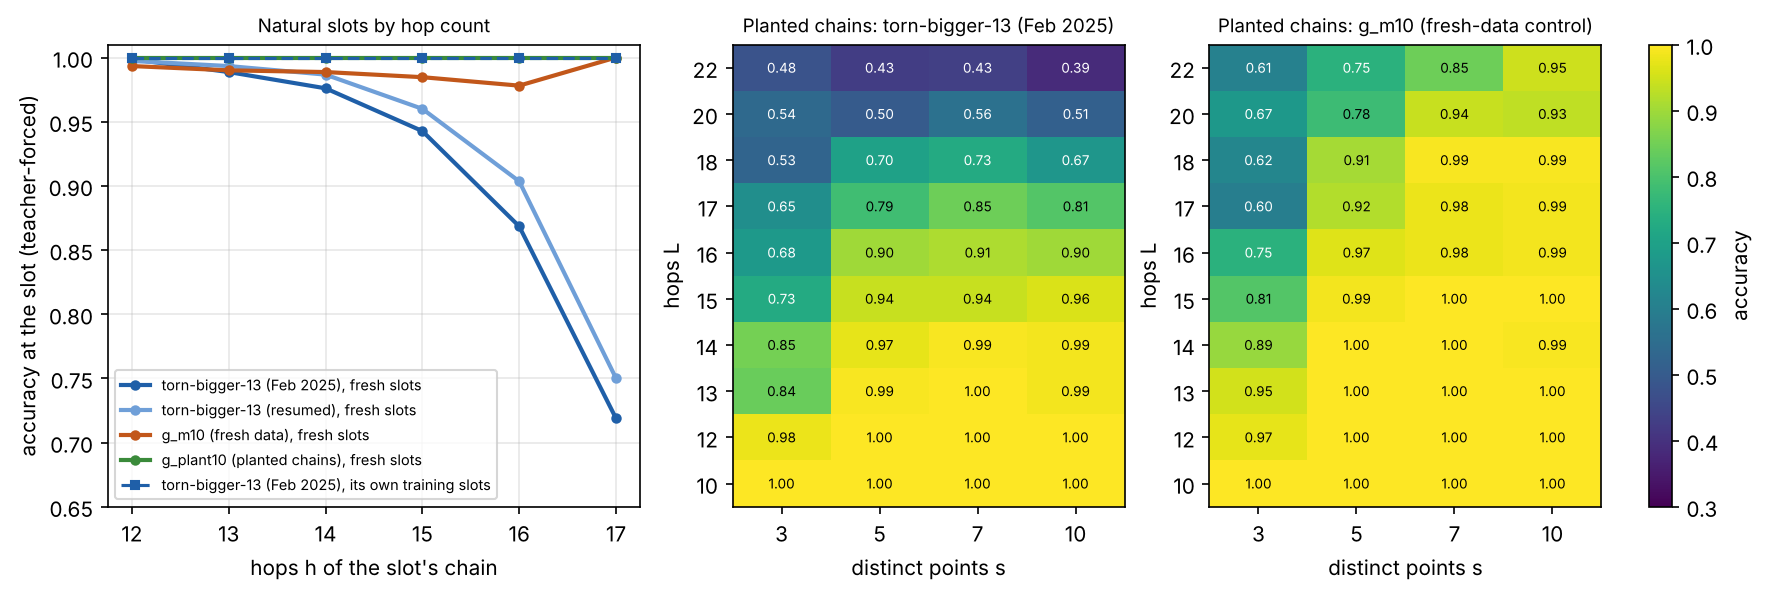
\includegraphics[width=1.00\linewidth]{fig_memorisation.png}\caption{Left: accuracy on natural slots by hop count, fresh slots for four models and \code{torn-\allowbreak{}bigger-\allowbreak{}13}’s own training slots. Middle and right: planted chains by hops $L$ and distinct points $s$, 150 words per cell, for \code{torn-\allowbreak{}bigger-\allowbreak{}13} (February 2025) and the fresh-data control.}\end{figure}

\lead{Hops against points} (\code{hop\_\allowbreak{}points\_\allowbreak{}grid.\allowbreak{}py}, planted chains,
150 words per cell, standard error about 4 points in the middle of the range). Accuracy for $s$ = 3 / 5 / 7 / 10
distinct points:

{\small\nopagebreak[4]
\begin{longtable}{@{}r l l@{}}
\toprule
\hdr{hops $L$} & \hdr{\code{torn-\allowbreak{}bigger-\allowbreak{}13} (Feb 2025)} & \hdr{\code{g\_\allowbreak{}m10} (fresh-data control)} \\
\midrule
\endfirsthead
\toprule
\hdr{hops $L$} & \hdr{\code{torn-\allowbreak{}bigger-\allowbreak{}13} (Feb 2025)} & \hdr{\code{g\_\allowbreak{}m10} (fresh-data control)} \\
\midrule
\endhead
\bottomrule
\endlastfoot
12 & 0.98 / 1.00 / 1.00 / 1.00 & 0.97 / 1.00 / 1.00 / 1.00 \\
13 & 0.84 / 0.99 / 1.00 / 0.99 & 0.95 / 1.00 / 1.00 / 1.00 \\
14 & 0.85 / 0.97 / 0.99 / 0.99 & 0.89 / 1.00 / 1.00 / 0.99 \\
15 & 0.73 / 0.94 / 0.94 / 0.96 & 0.81 / 0.99 / 1.00 / 1.00 \\
16 & 0.68 / 0.90 / 0.91 / 0.90 & 0.75 / 0.97 / 0.98 / 0.99 \\
17 & 0.65 / 0.79 / 0.85 / 0.81 & 0.60 / 0.92 / 0.98 / 0.99 \\
18 & 0.53 / 0.70 / 0.73 / 0.67 & 0.62 / 0.91 / 0.99 / 0.99 \\
20 & 0.54 / 0.50 / 0.56 / 0.51 & 0.67 / 0.78 / 0.94 / 0.93 \\
22 & 0.48 / 0.43 / 0.43 / 0.39 & 0.61 / 0.75 / 0.85 / 0.95 \\
\end{longtable}}

\code{g\_\allowbreak{}plant10} is at 1.00 in every cell; the resumed
\code{torn-\allowbreak{}bigger-\allowbreak{}13} is ahead of the February model in all 24 cells from 15 to 22
hops, by 2 to 18 points (\S\,\ref{sec:3.18}).

\lead{The elementary models} (\code{elem\_\allowbreak{}memorisation.\allowbreak{}py}). The same test with slots
binned by hop count (40–49 up to 80 or more), 300 per bin: training slots from 2M words of the boosted training
data, the validation file, and fresh slots from the matched generator. Accuracy, training / validation / fresh:

\begin{center}\small
\begin{tabular}{@{}>{\raggedright\arraybackslash}p{2.6cm} >{\raggedright\arraybackslash}p{3.4cm}
>{\raggedright\arraybackslash}p{3.6cm} >{\raggedright\arraybackslash}p{3.6cm}@{}}
\toprule
\hdr{model} & \hdr{wandb final validation loss over training loss} & \hdr{60–69 hops} & \hdr{70–79 hops (158, 13 and 300 slots)} \\
\midrule
\code{rerun-\allowbreak{}4} & 3,189 & 1.000 / 0.997 / 0.997 & 1.000 / 1.000 / 1.000 \\
\code{boosted-\allowbreak{}2} & 701 & 1.000 / 0.993 / 1.000 & 1.000 / 1.000 / 0.983 \\
\code{rerun-\allowbreak{}3} & 880 & 0.997 / 0.997 / 0.993 & 0.994 / 1.000 / 0.980 \\
\code{boosted-\allowbreak{}4} & 40 & 1.000 / 1.000 / 1.000 & 1.000 / 1.000 / 0.997 \\
\code{boosted-\allowbreak{}1} & 2.4 & 1.000 / 1.000 / 1.000 & 1.000 / 1.000 / 1.000 \\
\bottomrule
\end{tabular}
\end{center}

The 40–59 bins are at 0.997–1.000 for every model and source, and the median margins of the three sources agree
within about one logit in every bin. Whether the committed training files are what the December reruns trained
on is checked only weakly
(\code{elem\_\allowbreak{}train\_\allowbreak{}val\_\allowbreak{}check.\allowbreak{}py}:
\code{rerun-\allowbreak{}4} fits words from them more tightly than its validation words, $4.4\times10^{-7}$
against $1.6\times10^{-4}$ per slot; for the others a 3,000-word sample cannot tell), but their size and folder
match.

\begin{findbox}{What it shows}
\begin{itemize}
\item \lead{\code{torn-\allowbreak{}bigger-\allowbreak{}13} is right on every long chain it was trained on and
  not on fresh ones.} The differences are significant at every $h$ from 13 to 16 (Fisher’s exact test, $p$ from
  $3\times10^{-5}$ to 0.02). Up to 12 hops the margins of training and fresh slots agree (18.8 and 18.8); from
  13 they part (at 15 hops the 10th-percentile margin is 11.3 on training slots and 2.7 on fresh ones). So the
  model has memorised its long chains, and its general rule is reliable only to about 13 hops.
\item \lead{The decline starts inside the range the file covers.} The file holds 1,468 slots with 14 hops and
  270 with 15, yet 2 to 6\% of fresh ones are wrong. The cliff is not “beyond the data” (versions 4 to 7 said it
  was, \S\,\ref{sec:5} item 11).
\item \lead{The original fails by hops, the control by points.} For chains through 5, 7 or 10 points the
  original’s columns agree within the noise at every length; the control is near perfect through 10 points up to
  22 hops and loses accuracy as the chain revisits fewer points. These are qualitatively different weaknesses.
\item \lead{Confidence tells the same story.} The original’s median margin on fresh slots falls from 18.8 at 12
  hops to 9.5 at 16; the control’s from 12.1 to 8.6; \code{g\_\allowbreak{}plant10}’s stays at 14.4–14.7 from 12
  to 17 hops, on fresh slots and on \code{torn-\allowbreak{}bigger-\allowbreak{}13}’s training slots alike.
\item \lead{The elementary models do not do this.} In all five, training, validation and fresh slots are alike
  at every hop count, although four end with a validation loss 40 to 3,000 times their training loss
  (\S\,\ref{sec:3.18}). So memorising long chains is not a general effect of a static training file, and the
  loss gap is not by itself a sign of it.
\end{itemize}
\end{findbox}

\begin{findbox}{What this does and does not say}
\begin{itemize}
\item The original’s hop limit is a limit of the rule it learned (fresh chains), not of what it stores (its
  training chains are all right) and not of the architecture (\S\,\ref{sec:3.14}).
\item The most coherent account I have: a rule that composes chains to about 13 hops, the reach of the probe
  staircase at layer 5 (\S\,\ref{sec:3.9}), and memorised long chains on top. Once the training file is fit to a
  loss of about $10^{-9}$ no gradient is left to improve the rule. This is a hypothesis.
\item Whether the rule was ever longer and was lost when the model memorised, or was never longer, the final
  checkpoint cannot say; snapshots during a faithful rerun would (\S\,\ref{sec:6.1}).
\item Why the control learned a longer rule I do not know; it differs from the original run in more than the
  data (\S\,\ref{sec:3.14}).
\end{itemize}
\end{findbox}

\begin{limbox}{Limits}
One checkpoint per model and one seed; 228 and 32 fresh slots at 16 and 17 hops; only 34 training slots at 16
hops and 4 beyond; teacher-forced at one slot.
\end{limbox}

\subsection{The Spartan model folder: block boundaries in other runs, and which checkpoint is
which}\label{sec:3.18}
You uploaded the model folder from Spartan (206 checkpoints, the final epoch of every run since mid-2024), and
wandb histories for 15 of the runs. Details, tables for every model and the scripts are in
\code{snapshot-\allowbreak{}survey/\allowbreak{}README.\allowbreak{}md}; configs come from the git history of
\code{Midataur/\allowbreak{}permutations}.

\lead{Reading the older checkpoints.} Every model before
\code{elem-\allowbreak{}partitioned-\allowbreak{}long-\allowbreak{}boosted-\allowbreak{}1} (11 Feb 2025) has one
extra multi-head attention layer applied to the embeddings before the blocks, with no layer norm and no residual
connection (\code{LEGACY\_\allowbreak{}ARCHITECTURE}), and some were trained with other attention masks, which
the checkpoints store. \code{np\_\allowbreak{}transformer.\allowbreak{}py} now handles both.

\lead{Which \code{torn-\allowbreak{}bigger-\allowbreak{}13}.} The file on Spartan was saved in float32 on 29 Nov
2025, after the resume; the repo checkpoint is bfloat16, like every February save, and every trained weight
differs from the Spartan file. So this report is about the February model (161 epochs), presumably the paper’s.
The resumed model has the same shape of hop limit, is a little better at 15 to 22 hops (\S\,\ref{sec:3.17}), and
still gets 99.3–100\% of its training slots.

\lead{The block boundary in other runs} (\code{block\_\allowbreak{}survey.\allowbreak{}py}: for each $k$, how
much rows $k$ and $k+1$ of the position-cosine matrix differ away from the diagonal, as a robust $z$-score;
Figure 5b’s model has $z\approx5$ at 72–73, untrained models at most 2.5):

{\small\nopagebreak[4]
\begin{longtable}{@{}>{\raggedright\arraybackslash}p{5.2cm} r >{\raggedright\arraybackslash}p{2.6cm} r
>{\raggedright\arraybackslash}p{3.2cm}@{}}
\toprule
\hdr{run} & \hdr{seed} & \hdr{epochs (wandb)} & \hdr{test slots right} & \hdr{boundary} \\
\midrule
\endfirsthead
\toprule
\hdr{run} & \hdr{seed} & \hdr{epochs (wandb)} & \hdr{test slots right} & \hdr{boundary} \\
\midrule
\endhead
\bottomrule
\endlastfoot
\code{elem-\allowbreak{}partitioned-\allowbreak{}long-\allowbreak{}boosted-\allowbreak{}1} (Figure 5b) & 42 & 96 & 99.99\% & 72–73 ($z$ 4.9) \\
\code{elem-\allowbreak{}partitioned-\allowbreak{}long-\allowbreak{}boosted-\allowbreak{}2} & 43 & 63 & 100.00\% & 81 ($z$ 5.8) \\
\code{elem-\allowbreak{}partitioned-\allowbreak{}long-\allowbreak{}boosted-\allowbreak{}4} & 97 & 341 & 100.00\% & none \\
\code{rerun-\allowbreak{}2} (Dec 2025) & 42 & 193 & 99.91\% & weak, about 79 ($z$ 3.9) \\
\code{rerun-\allowbreak{}3} (Dec 2025) & 43 & 193 & 99.99\% & 78 ($z$ 7.3) \\
\code{rerun-\allowbreak{}4} (Dec 2025) & 44 & 193 & 99.99\% & none \\
\code{elem-\allowbreak{}partitioned-\allowbreak{}long-\allowbreak{}14} (older data and architecture) & 42 & 150 & 98.28\% & 69 ($z$ 15.6) \\
\code{elem-\allowbreak{}partitioned-\allowbreak{}long-\allowbreak{}11}, \code{-\allowbreak{}12} (same) & 42 & 332, 276 & 98.2–98.3\% & none \\
\code{e\_\allowbreak{}base} (\S\,\ref{sec:3.15}) & 0 & 109M fresh words (about 7 epochs’ worth) & 99.58\% & none \\
\end{longtable}}

\code{elem-\allowbreak{}partitioned-\allowbreak{}long-\allowbreak{}boosted-\allowbreak{}3} and
\code{rerun-\allowbreak{}1} are left out: the first was restarted from scratch under the same name (its last
logged epoch repeats epoch 1), the second ran 7 epochs; their checkpoints are early ones.

\begin{findbox}{What it shows}
\begin{itemize}
\item \lead{The boundary is common but not fixed.} Three of six fully trained runs with Figure 5b’s config have
  a clear boundary, one a weak one and two none; the places are 72, 78, 79 and 81, and an older run has one at
  69. It does not follow the length of training (63 to 341 epochs) or the accuracy, and the same seed did not
  give the same result in February and December (seed 42: 72, then a weak 79), when the code and environment had
  changed.
\item \lead{The first layers use it.} For attention between word positions at most 6 apart, several heads of
  block 1 (and some of block 2) put far less weight across the boundary than across other places
  (\code{block\_\allowbreak{}attention.\allowbreak{}py}: \code{boosted-\allowbreak{}1} b1h0 at 0.13 of its
  average, \code{boosted-\allowbreak{}2} b1h5 at 0.05, \code{rerun-\allowbreak{}3} b1h5 at 0.14,
  \code{long-\allowbreak{}14} all six heads of block 1 at 0.04 to 0.56). In \code{boosted-\allowbreak{}4},
  without a boundary, no early head dips near 72; \code{rerun-\allowbreak{}4}, also without one, has a single
  block-1 head with a dip at 82.
\item \lead{Chains across it are not harder}
  (\code{block\_\allowbreak{}crossing\_\allowbreak{}test.\allowbreak{}py}): 24 hops inside 40 positions centred
  on the boundary are followed as well as inside the left block (\code{boosted-\allowbreak{}1} 1.000 and 1.000,
  \code{rerun-\allowbreak{}3} 0.937 and 0.997, \code{long-\allowbreak{}14} 0.630 and 0.697); the later blocks
  bridge the split, as the position swaps of \S\,\ref{sec:3.8} suggested.
\item \lead{No other general model helps with the cliff.} \code{torn-\allowbreak{}bigger-\allowbreak{}5} to
  \code{-\allowbreak{}8} and \code{-\allowbreak{}10} to \code{-\allowbreak{}12} never left the plateau (at most
  73\% of training slots in 75 to 286 epochs); \code{torn-\allowbreak{}bigger-\allowbreak{}9}’s 100\% at 24 hops
  comes from a mask that lets the word positions see the teacher-forced answers.
  \code{torn-\allowbreak{}bigger-\allowbreak{}13} is the only general model trained with the original recipe
  that learned the task.
\end{itemize}
\end{findbox}

\begin{limbox}{Limits}
Final checkpoints only; one run per seed and setup; the boundary detector is a summary of a matrix that can have
other structure (the “chevron” patterns of
\code{fig\_\allowbreak{}block\_\allowbreak{}survey.\allowbreak{}png}).
\end{limbox}

% ====================================================================================================
% 4 What this means for the density idea [UPDATED]
% ====================================================================================================
\section{What this means for the density idea \tagupd{}}\label{sec:4}
\begin{itemize}
\item The algebraic reason the target is local (Moore’s presentation: every relation involves at most 4 points,
  and the pointer chase needs one point at a time) stands. The experiments above don’t test it directly.
\item What the data does say is that the model’s generalization beyond the training support is real at the level
  of whole words (all 2,000 real test words touch 17 or more points, against at most 10 in training), while each
  output slot only needs a short chase (at most 9 distinct points in the real test file). The original model’s
  ability to follow fresh chains falls off from about 13 to 15 hops, while it is right on every long chain of
  its own training file (\S\,\ref{sec:3.17}); version 9 said the fall was where the training data runs out of
  long chains, which \S\,\ref{sec:3.17} contradicts. Crossing the support boundary ($s=10\to11$) costs only 2 to
  4 points. An accurate statement of what training “covers” is therefore about \textbf{chain length (hop count)}
  much more than about how many distinct points a word or a trajectory touches. \S\,\ref{sec:3.14} qualifies
  this: a control trained on the same distribution with fresh data does not show the cliff, and the weak spots
  it does show are in the pair (hops, distinct points), chains through few points, so what training covers is
  hops and distinct points together. \S\,\ref{sec:3.17} adds that the two models fail differently: the original
  by hops whatever the points, the control only on chains through few points.
\item In the spirit of the $\mathbb{Q}\subset\mathbb{R}$ analogy: the objects that need to be dense are
  trajectories (chases), not words. The training distribution is dense in short chains, wherever they sit among
  25 points, and sparse in long ones. A density argument would need a metric in which “long chain” is far from
  “short chain”. \S\,\ref{sec:3.17} adds a distinction such an argument needs: what the data contain is not what
  the learned rule covers. \code{torn-\allowbreak{}bigger-\allowbreak{}13}’s file contains chains of up to 18
  hops and the model is right on all of them, but its rule extends to fresh chains only up to about 13 hops; the
  fresh-data control, which saw about as few chains of 18 or more hops (10 slots in its whole run), follows
  fresh chains through 10 points to 22 hops. So density of the training sample in (hops, points) is necessary
  for an argument of this kind but not sufficient: the argument has to say which chains the model generalises
  to, and for the original model that is fewer than the data contain.
\item The training experiment (\S\,\ref{sec:6.1}) separates the two readings for the general model: with long
  chains in the data a five-block model gets 24 of 24 hops, so five blocks are not what limits it
  (\S\,\ref{sec:3.14}). \S\,\ref{sec:3.9}–\ref{sec:3.10} had made the depth reading more plausible than I judged
  in version 4 and \S\,\ref{sec:3.11} had qualified that; \S\,\ref{sec:3.14} settles it within the range a
  25-letter word can test. That rules out a limit of the architecture, not that
  \code{torn-\allowbreak{}bigger-\allowbreak{}13} learned a rule limited by its depth: its accuracy on fresh
  chains falls with the number of hops whatever the number of points (\S\,\ref{sec:3.17}), from about where its
  probe staircase stops (\S\,\ref{sec:3.9}). What made it learn a short rule I do not know; the control, trained
  differently, learned a longer one (\S\,\ref{sec:3.14}).
\item Seven results from \S\,\ref{sec:3.6}–\ref{sec:3.14} bear on this. (i) The elementary model, trained on far
  longer chases than the general model, shows no hop-count cliff up to 80 hops and loses accuracy only beyond
  the widths it was trained on. That supports reading the general model’s cliff as a coverage effect in hop
  count, though the two tasks differ, and the elementary model’s hops are $\pm1$ steps inside a window of at
  most 11 positions, which may be composed differently. Test 13 (\S\,\ref{sec:3.13}) adds that the elementary
  model also follows chains of 100 to 118 hops, longer than any in my sample of its training data. (ii) The
  interventions say the general model is local in the sense the algebra suggests: for $L\le12$ the output
  depends on the chase letters and nothing else. (iii) The probes at the query position say it does not hold the
  chain’s later states (\S\,\ref{sec:3.6}); the probes and patching at the word positions say they are built
  there, layer by layer, with a reach of roughly 1, 1, 4, 8 and 13 or more hops at layers 1 to 5, and read in
  the last block (\S\,\ref{sec:3.9}–\ref{sec:3.10}). (iv) If that is how five blocks compose chains, the hop
  limit may be set by depth, and more long chains in the data would not move it, while a deeper model would.
  \S\,\ref{sec:3.14} refutes this: planted chains moved the limit beyond 24 hops with the same five blocks. (v)
  The elementary model has the same word-position staircase (about 1, 2, 4, 8 and 12 hops at layers 1 to 5) and
  still follows 80 hops (\S\,\ref{sec:3.11}), so a per-position reach of about $2^\ell$ does not by itself cap
  the hop length, and (iv) is weaker than I wrote in version 5. (vi) The heads that link hop letters are needed
  more as chains get longer, in both models, and in the elementary model the hop offsets they attend to double
  with depth (\S\,\ref{sec:3.12}); but I did not find how its 80 hops are composed, so (iv) is not settled
  either way. (vii) The training run (\S\,\ref{sec:3.14}): long chains in the data remove the cliff at five
  blocks (24 of 24 hops, including chains through up to 25 points, outside the 10-point support), the control
  trained on the original distribution has no cliff at 20 hops, and the retrained models do not show the probe
  staircase or the hop-offset doubling of the others (\S\,\ref{sec:3.16}). A density argument built on chains
  would then need to be about what the data contain, in hops and in distinct points together, and not about the
  architecture: up to 24 hops, which is all a 25-letter word can test, I found no limit that five blocks set.
  How the model composes the chains I did not find. (viii) \S\,\ref{sec:3.17}: the original’s limit is in what
  it learned to generalise, not in what it stored; it knows every long chain of its file. A density argument
  therefore has to be about the chains a training procedure makes the model generalise to, which for the
  original recipe is fewer than the data contain.
\end{itemize}

\subsection{What algorithm I think the general model learned \tagnew{}}\label{sec:4.1}
This is an interpretation that puts together \S\,\ref{sec:3.6}–\ref{sec:3.18}. No single test shows it, and the
parts I am least sure of are marked.

\lead{The task, in the pointer picture (\S\,\ref{sec:3.1}).} Output slot $k$ is where a pointer that starts at
$k$ ends up when the word’s letters are read from right to left, each letter $(a,b)$ moving the pointer if it
sits on $a$ or $b$. Only the letters that move the pointer (the hop letters) matter. The answer for slot $k$ is
the end of a chain of hop letters, each of which shares a point with the next.

\lead{What I think \code{torn-\allowbreak{}bigger-\allowbreak{}13} computes.}

\begin{enumerate}
\item \lead{At the word positions: suffix composition.} For each letter, and each of its two endpoints, the
  model builds the letter’s \emph{continuation}: where a pointer that leaves the letter there ends up after the
  letters to its left (\S\,\ref{sec:3.9}). Letters are linked to the next and previous letter on their chain by
  content: heads in blocks 1–3 attend to letters that share a point, not to fixed offsets (\S\,\ref{sec:3.12},
  the natural-word control). Several heads do this redundantly: no single one is needed at 8 hops, but the four
  together are (\S\,\ref{sec:3.13}).
\item \lead{The reach grows faster than one hop per layer.} The continuation is linearly readable about 1, 1, 4,
  8 and 13 or more hops ahead after layers 1 to 5 (\S\,\ref{sec:3.9}). That is the pattern of pointer jumping
  (each layer a letter joins its continuation to the continuation of the letter at the end of it, roughly
  doubling the reach), not of one hop per layer, which would give 5. The general model’s attention offsets show
  this only weakly (mostly $\pm1$ hop, one head at $+2$ and $+4$, \S\,\ref{sec:3.12}), so the exact composition
  step is not pinned down. In the elementary model the doubling is clear in both the probes and the attention
  offsets ($\pm1$, $\pm2$, $\pm4$, then $\pm6$ to $\pm12$ by block 4, \S\,\ref{sec:3.11}–\ref{sec:3.12}).
\item \lead{At the query position: find the first hop, read its continuation.} The output position for slot $k$
  takes in the first hops of its chain early (patching the first hop stops helping after block 3,
  \S\,\ref{sec:3.10}). It does not hold the chain’s later states in linearly readable form (\S\,\ref{sec:3.6}).
  In the last block it reads the answer off the word positions: restoring the word positions after block 4
  restores the answer for a corrupted middle or last hop in every word (\S\,\ref{sec:3.10}).
\item \lead{The limit is the reach.} If the continuation stored at the chain’s first letters covers the whole
  chain, the answer is right; if the chain is longer than the reach the layers have built, it is not. This
  predicts a limit in hops, not in points, at about the layer-5 reach. That is what \S\,\ref{sec:3.17} finds on
  fresh chains: about 0.99 to 13–14 hops, then a steady fall, the same through 5, 7 or 10 points.
\item \lead{Long training chains are stored separately.} \code{torn-\allowbreak{}bigger-\allowbreak{}13} is
  right on all its training chains of 14 to 18 hops (\S\,\ref{sec:3.17}), beyond the reach of its rule. So for
  those it has something else, a memorised association for those particular words, which does not transfer to
  fresh ones. How it is stored I did not look at.
\end{enumerate}

\lead{What I am least sure of.}

\begin{itemize}
\item The doubling step itself in the general model (point 2): the probes show the reach, but the attention
  offsets do not show how it is achieved.
\item Whether the query reads one continuation or combines several (points 3 and 4).
\item Whether the rule was ever longer during training and was overtaken by memorisation, or was never longer
  (\S\,\ref{sec:3.17}; snapshots of a faithful rerun would answer it).
\end{itemize}

\lead{The other models.}

\begin{itemize}
\item \lead{The elementary model} fits the same scheme with clean doubling, and its reach at layer 5 (about 12
  hops in its probe, \S\,\ref{sec:3.11}) is far below the 80 to 118 hops it follows. So either the reach is
  underestimated by a linear probe or its windows (at most 11 positions) let it compose differently. I cannot
  decide this.
\item \lead{The planted model (\code{g\_\allowbreak{}plant10})} does not show the staircase (\S\,\ref{sec:3.16})
  and its confidence does not depend on chain length at all (\S\,\ref{sec:3.17}: median margin 14.4–14.7 from 12
  to 17 hops, and 100\% to 24 hops). Whatever it does is not limited by a reach that grows with depth. I did not
  find its algorithm.
\item \lead{The fresh-data control (\code{g\_\allowbreak{}m10})} follows chains through 10 points to 22 hops but
  fails on chains that keep revisiting 3 to 5 points (\S\,\ref{sec:3.17}). That suggests a computation organised
  around points rather than letters (for example, tracking the last letter that touched each point). This is a
  guess.
\end{itemize}

\subsection{What notion of density fits the results \tagnew{}}\label{sec:4.2}
The aim is a statement of the form “the training distribution is dense in the test distribution in a sense that
explains why the model generalises”, in the spirit of $\mathbb{Q}\subset\mathbb{R}$. Here is the notion I think
the results support, built in three steps, each from a result.

\lead{Step 1: the objects are slots, through their chains, up to relabelling.} Three results fix this.

\begin{itemize}
\item \lead{Locality.} The output at a slot depends only on its hop letters (\S\,\ref{sec:3.7}: replacing every
  other letter leaves 98–100\% of predictions unchanged for $L\le12$).
\item \lead{Symmetry.} The token embeddings are close to $S_{25}$-invariant (\S\,\ref{sec:3.5}), and the
  training words are 10-point words relabelled into all 25 labels.
\item \lead{Pattern.} So the natural object is the \emph{chain pattern} of a slot: the sequence of points the
  pointer visits, up to relabelling (a walk with $L$ hops through $s$ distinct points, written as a string such
  as $a\,b\,a\,c\,b$), together with where the hop letters sit in the word.
\end{itemize}

Write $\pi(w,k)$ for the pattern of slot $k$ of word $w$. A training set $T$ and a test distribution $\mu$ then
define two distributions on patterns: $\pi_*T$ and $\pi_*\mu$.

\lead{Step 2: support in pattern space explains the paper’s result.} Every test word touches 17 to 25 points,
outside the 10-point training support (\S\,\ref{sec:2.3}). But every slot of the real test file has a chain of
at most 9 hops through at most 9 points (\S\,\ref{sec:1} item 3). Every such pattern fits in 10 points and
occurs, under every relabelling, in the training data, and often: 0.8\% of training slots have 10 or more hops
(Binomial(25, 0.18)), while a slot of a uniform 25-point test word has about 2 hops on average (Binomial(25,
0.077)).

So the paper’s generalisation from $S_{10}$ to $S_{25}$ needs no extrapolation at all in pattern space:
$\pi_*\mu_{\text{test}}$ is supported inside $\pi_*T$, and the model is right there (\S\,\ref{sec:3.2}). This is
the sense in which the training set is “dense”: not as words, but as patterns of the slots, modulo the symmetry.
It is the analogue of $\mathbb{Q}\subset\mathbb{R}$ with a much simpler topology: the relevant space is discrete
and the test patterns are literally contained, with plenty of examples each.

\lead{Step 3: containment is not enough; frequency and the training procedure decide the edge.} At long chains
the two runs on the same distribution disagree.

{\small\nopagebreak[4]
\begin{longtable}{@{}r >{\raggedleft\arraybackslash}p{1.9cm} >{\raggedleft\arraybackslash}p{2.2cm}
>{\raggedleft\arraybackslash}p{2.4cm} >{\raggedleft\arraybackslash}p{2.5cm}
>{\raggedleft\arraybackslash}p{2.5cm}@{}}
\toprule
\hdr{hops $h$} & \hdr{probability per slot} & \hdr{slots in the original’s 8M-word file} & \hdr{in the control’s 205M fresh words} & \hdr{\code{torn-\allowbreak{}bigger-\allowbreak{}13}, fresh slots} & \hdr{\code{g\_\allowbreak{}m10}, fresh slots} \\
\midrule
\endfirsthead
\toprule
\hdr{hops $h$} & \hdr{probability per slot} & \hdr{slots in the original’s 8M-word file} & \hdr{in the control’s 205M fresh words} & \hdr{\code{torn-\allowbreak{}bigger-\allowbreak{}13}, fresh slots} & \hdr{\code{g\_\allowbreak{}m10}, fresh slots} \\
\midrule
\endhead
\bottomrule
\endlastfoot
12 & $4.6\times10^{-4}$ & 36,000 & 930,000 & 0.999 & 0.993 \\
13 & $1.0\times10^{-4}$ & 8,000 & 205,000 & 0.989 & 0.990 \\
14 & $1.9\times10^{-5}$ & 1,500 & 39,000 & 0.976 & 0.989 \\
15 & $3.0\times10^{-6}$ & 240 & 6,200 & 0.943 & 0.985 \\
16 & $4.2\times10^{-7}$ & 33 & 850 & 0.868 & 0.978 \\
17 & $4.8\times10^{-8}$ & 4 & 99 & 0.72 & 1.00 (32 slots) \\
18 & $4.7\times10^{-9}$ & 0.4 & 10 &  &  \\
20–22 & $\le2.5\times10^{-11}$ & 0 & 0 & 0.4–0.5 (planted, 10 points) & 0.93–0.95 (planted, 10 points) \\
\end{longtable}}

(Probabilities are exact, Binomial(25, 0.18) per slot (\S\,\ref{sec:3.14}); the counts are expected values.)

\begin{itemize}
\item \lead{\code{torn-\allowbreak{}bigger-\allowbreak{}13} generalises where the data are dense and memorises
  where they are not.} Its rule is reliable while there are some $10^4$ training slots per hop count (12–13
  hops). Between about $10^3$ and a few (14–17 hops) the patterns are in its support, and it is right on all of
  them in training, but 2 to 28\% of fresh ones are wrong. So \emph{containment} of a pattern in the training
  set does not make the model generalise to it; \emph{frequency} does, for this recipe.
\item \lead{The control generalises beyond its data.} With about 25 times as many examples at every hop count it
  is reliable to 16–17 hops, and on planted chains through 10 points it is still at 0.93–0.95 at 20–22 hops,
  where it has seen no example at all. So its rule extends past the patterns it has seen. Its failures are at
  patterns with few distinct points (chains through 3 points: 0.6–0.75 from 16 hops), which are rare in every
  natural training set (about $4\times10^{-9}$ per slot for 16 hops through 3 points, \S\,\ref{sec:3.14}).
\item \lead{The elementary model is like the control:} it follows 100 to 118 hops, beyond the longest chain in
  my sample of its training data (78, \S\,\ref{sec:3.13}), and does not memorise its long chains
  (\S\,\ref{sec:3.17}).
\end{itemize}

\lead{The notion I would propose.} Two parts:

\begin{enumerate}
\item \lead{Coverage:} the set $C_N(T)$ of chain patterns, modulo relabelling, that occur at least $N$ times in
  the training set. A test distribution is covered at level $(N,\varepsilon)$ if $\pi_*\mu(\text{patterns
  outside } C_N(T))\le\varepsilon$. For the paper’s test file it is covered for any reasonable $N$ with
  $\varepsilon=0$.
\item \lead{Closure:} the patterns the trained model actually gets right on fresh words. That is $C_N(T)$
  extended by whatever the learned rule composes, $\overline{C}(T,\text{procedure})$. For
  \code{torn-\allowbreak{}bigger-\allowbreak{}13} it is smaller than the support of its data (it stops at about
  13 hops, below the 18 its file contains). For the control and the elementary model it is larger (to 22 and to
  118 hops). If \S\,\ref{sec:4.1} is right, the closure is the set of patterns whose chains fit within the reach
  built by the layers from frequent short segments. That suggests a form: chains that split into at most about
  $2^{\ell}$ frequent segments after $\ell$ layers.
\end{enumerate}

A density argument for generalisation then has two halves. The first, coverage, is a property of the data and
the symmetry and can be proved or counted; it is all the paper’s $S_{10}\to S_{25}$ result needs. The second,
closure, is a property of the training procedure as much as of the data, and I can only measure it
(\S\,\ref{sec:3.17}).

\lead{What this leaves open.}

\begin{itemize}
\item I have measured patterns only by $(L, s)$. The full pattern (the order of revisits, the gaps between hop
  letters) may matter at the edges; the control’s weakness on few-point chains is one sign that it does.
\item The threshold $N$ at which \code{torn-\allowbreak{}bigger-\allowbreak{}13} stops generalising (about
  $10^3$–$10^4$ slots per hop count) comes from one run, and the control shows it is not a property of the data
  alone.
\item Whether a larger static file moves the original’s edge (a single-change experiment) would say how much of
  the closure is frequency and how much is the recipe.
\end{itemize}

% ====================================================================================================
% 5 Corrections to my earlier messages
% ====================================================================================================
\section{Corrections to my earlier messages}\label{sec:5}
\begin{enumerate}
\item \lead{Ladder hypothesis.} I framed the ladder test around a boundary at 11 distinct points, the first
  beyond the $m=10$ support. That boundary is correct (\S\,\ref{sec:2.3}). There is no collapse at it (summary
  item 5).
\item \lead{Word length.} My earlier closed-form tail estimates assumed 24 letters. The config uses 25
  (\code{MAX\_\allowbreak{}TRANS\_\allowbreak{}NUMBER = 25}). Recomputed, the per-trajectory probability of at
  least 11 distinct points is $1.1\times10^{-6}$ (was $7.0\times10^{-7}$), and per word at most
  $2.7\times10^{-5}$ (was $1.7\times10^{-5}$). The simulation I ran earlier used 24 letters; the stratified run
  here uses 25 and saw none in 20,000 words, consistent with this.
\item \lead{Training support.} I assumed $m=10$, then switched to $m=16$ on the config’s say-so, and finally
  measured the real data: $m=10$ (\S\,\ref{sec:2.3}). The config’s
  \code{ACTUAL\_\allowbreak{}GROUP\_\allowbreak{}SIZE} does not describe the data.
\item \lead{Gram spectrum.} See \S\,\ref{sec:3.5}.
\item \lead{Untested:} my earlier suggestion that $m=4$ or $5$ might already suffice has not been tested (it
  needs retraining).
\item \lead{Leftover in \S\,\ref{sec:7}.} Version 1 of this report described the fixed-hop sweep as crossing an
  $s=16/17$ boundary in the file table in \S\,\ref{sec:7}. That was left over from the wrong $m=16$; the sweep
  crosses $s=10/11$, as \S\,\ref{sec:3.3} says. Fixed in version 2.
\item \lead{The block in Figure 5b.} In version 2 of \S\,\ref{sec:3.8} I said this checkpoint was not a clear
  example of the position-embedding block and that I had no seed that shows it. After finding that the saved
  picture in the original repo matches this checkpoint exactly, and you confirming it is Figure 5b, that was
  wrong. The blocks are at 72 and 120, not 45 (\S\,\ref{sec:3.8}).
\item \lead{Coverage versus depth.} In version 4 (\S\,\ref{sec:1} item 12, \S\,\ref{sec:4}, \S\,\ref{sec:6} item
  1) I said that the elementary model’s results favoured “rare in training” over “five layers cannot do it”, and
  called training on long-chain-enriched data “now more motivated”. The probes and patching at the word
  positions (\S\,\ref{sec:3.9}–\ref{sec:3.10}) show a depth-like staircase, so I no longer lean either way: it
  is open, and \S\,\ref{sec:6.1} is designed to settle it.
\item \lead{The depth reading of \S\,\ref{sec:3.9}.} In version 5 I wrote that the staircase of
  \S\,\ref{sec:3.9} (about 1, 1, 4, 8 and 13 or more hops at layers 1 to 5) was “a reason to take a depth limit
  seriously”, because about $2^\ell$ hops per layer would cap five blocks near 16 hops. The elementary model has
  the same staircase at its word positions and follows 80 hops (\S\,\ref{sec:3.11}). So the staircase is
  compatible with a depth limit but is not evidence for one by itself; I have marked the sentence in
  \S\,\ref{sec:3.9} and the point in \S\,\ref{sec:4}.
\item \lead{Two first readings of the attention numbers.} (a) At first I called heads that put 30 to 40 times
  the uniform attention on the next or previous hop letter “next-hop” and “previous-hop” heads. In planted words
  most letters are chain letters, so a head that only looks at the nearest letters on one side would give the
  same numbers. The control on natural words (\S\,\ref{sec:3.12}) shows that the best of these heads do prefer
  the hop letter to non-chain letters at the same distance (3 to 4 times in the general model, 13 to 40 times in
  the elementary model), but against decoys (non-chain letters that hold the same point) the ratio is only about
  1.1 to 4 in the general model and 2 to 4 for most of those elementary heads, and 1.1 to 1.3 for block 1 heads
  1 and 3 of the elementary model. So what some of these heads follow is partly “a letter that holds the point I
  am at”, not only “the next letter on the chain”. (b) I first read the query’s attention (block 5 head 1 of the
  elementary model, mass peak at hop about 28 at $L=80$) as a rule about hop number. It reads a fixed range of
  word positions (72 to 83); the hop number grows with $L$ only because longer chains put more hops in the same
  positions.
\item \lead{Four things I said or assumed around the training run.} (a) \emph{Tail frequencies.} In a message I
  gave the chance of 14 or more hops per slot as $1.2\times10^{-5}$ and of 16 or more as $10^{-6}$ (from a
  sample of 1M slots), and said that chains of 18 or more hops essentially never occur in the control’s data.
  The number of hops is exactly Binomial(25, 0.18); the exact values are $2.2\times10^{-5}$ and
  $4.7\times10^{-7}$, a 4M-slot simulation agrees, and the control saw about 10 slots with 18 or more hops
  (\S\,\ref{sec:3.14}). (b) \emph{Testing beyond the longest trained chain.} I said I could test
  \code{g\_\allowbreak{}plant10} beyond its longest training chain. A 25-letter word cannot hold a chain longer
  than the 25 hops it was trained on, so this is impossible; the beyond-the-edge tests are the control
  (\S\,\ref{sec:3.14}) and Test 13 (\S\,\ref{sec:3.13}). (c) \emph{The depth prediction.} I wrote that
  \code{g\_\allowbreak{}plant10} would still fall off between 16 and 24 hops if depth were the limit, and that
  the 8-block arm would not. That design cannot show a depth limit once the five-block planted model is at the
  ceiling, which it was; a model with fewer blocks (the 3-block optional arm of \S\,\ref{sec:6.1}) is the
  informative one, and I should have made it a main arm. (d) \emph{Where the cliff sits.} Versions 4 to 7 said
  that the general model’s cliff sits where its training data ends (\S\,\ref{sec:3.3}, \S\,\ref{sec:4}). The
  control extrapolates two to four hops beyond that point (\S\,\ref{sec:3.14}), so the end of the training
  chains is not by itself the explanation.
\item \lead{How I compared the data of the original and the retrained models (\S\,\ref{sec:3.14},
  \S\,\ref{sec:3.15}).} In version 8 I wrote that the original general model saw 1.3 billion word views against
  205M for the control, and that the original elementary model saw 14 times as many word views as
  \code{e\_\allowbreak{}base}. Those are counts of words presented (epochs times file size), and I used them as
  if they measured how much data each model had. By distinct words the order is the reverse: the original
  general model saw 8M distinct words and the control 205M (25 times as many); the original elementary model saw
  16M and \code{e\_\allowbreak{}base} 109M (about 7 times as many). Both counts are now given in a table in
  \S\,\ref{sec:3.14}, and \S\,\ref{sec:1} items 21 and 23, \S\,\ref{sec:3.14} and \S\,\ref{sec:3.15} say which
  of them each statement is about. You pointed this out.
\item \lead{Things versions 8 and 9 and my messages got wrong or overstated.} (a) \emph{bfloat16.} Version 9
  listed bfloat16 among the differences between the control and the original run; the original also used it
  (\S\,\ref{sec:3.14}). (b) \emph{The seed.} In a message I gave the original run’s seed as 44 (from the current
  \code{config.\allowbreak{}py}); \code{torn-\allowbreak{}bigger-\allowbreak{}13}’s config has 42. (c)
  \emph{Which checkpoint.} In a message I said the analysed \code{torn-\allowbreak{}bigger-\allowbreak{}13} was
  “almost certainly” the model after the November 2025 resume (185 epochs); it is the February model (161
  epochs, \S\,\ref{sec:3.18}). (d) \emph{The elementary loss gap.} In a message I said the elementary run’s lack
  of a gap between training and validation loss fitted the memorisation reading; that holds only for
  \code{elem-\allowbreak{}partitioned-\allowbreak{}long-\allowbreak{}boosted-\allowbreak{}1}, and the other
  elementary runs have large gaps and no memorisation of long chains (\S\,\ref{sec:3.17}). (e) \emph{What the
  training run showed.} Version 8 (written by an earlier model in this conversation) said that planted chains
  “remove the cliff” and that the depth reading was “refuted”, and called the coverage prediction “confirmed”.
  The control has no cliff either, so the planted arm removes nothing it had; the run refutes a limit of the
  architecture, not of the rule the original learned; and the coverage prediction was met by the planted arm and
  nearly by the control (\S\,\ref{sec:1} items 6, 12 and 20). (f) \emph{Internals.} Version 8 said the planted
  models “organise the work differently” and that the original “does not keep a step-by-step record”; both rest
  on linear probes, one seed and zero ablation, and are now stated as differences in measurements and as not
  linearly decodable (\S\,\ref{sec:1} items 9 and 22).
\end{enumerate}

% ====================================================================================================
% 6 Not done, and suggested next steps
% ====================================================================================================
\section{Not done, and suggested next steps}\label{sec:6}
\lead{Inference-only tests run in this version:} Test 16 and the hops-against-points grid (\S\,\ref{sec:3.17}),
and the survey of the Spartan model folder (\S\,\ref{sec:3.18}); before them, layer-wise probes
(\S\,\ref{sec:3.6}), irrelevance interventions (\S\,\ref{sec:3.7}), the elementary-transposition port with
baseline, width and hop-count tests (\S\,\ref{sec:3.8}, Tests 6a and 6b), probes and activation patching at the
word positions (\S\,\ref{sec:3.9}, \S\,\ref{sec:3.10}), the same two tests on the elementary model
(\S\,\ref{sec:3.11}), and attention patterns and single-head ablation of both models (\S\,\ref{sec:3.12}). In
this version: the elementary model beyond its longest training chase and zeroing groups of heads of the general
model (\S\,\ref{sec:3.13}), and probes, attention, ablation, greedy ablation and patching on the four retrained
models (\S\,\ref{sec:3.16}).

\lead{Inference-only tests not yet run:} gap/alignment variations beyond spread versus contiguous; weight-level
equivariance; removing the block structure itself from the elementary model’s position embeddings (for example
by projecting out the directions that separate the blocks), and swaps involving the 16 output positions
(\S\,\ref{sec:3.8}). Patching the general model for $L=20$ and above (the elementary model is patched up to
$L=80$, \S\,\ref{sec:3.11}). Patching one head or one component at a time (head groups are now ablated,
\S\,\ref{sec:3.13} and \S\,\ref{sec:3.16}), which would say what the heads of \S\,\ref{sec:3.12} carry and how
24 hops (the planted models) and 80 hops (the elementary model) are composed.

\lead{Needs training (not possible in my environment):} done once on Spartan (\S\,\ref{sec:3.14}):
long-chain-enriched data, an 8-block model and a control, one seed each. Still open: more seeds; a model with
fewer blocks as the depth test (3 blocks on the planted data); the control trained longer or with a constant
learning rate (its planted-slot accuracy was still rising); a control with the original’s batch size, schedule
and repeated 8M-word file, to see whether the cliff comes back; the support-size sweep (planted chains on 5
points); and \code{e\_\allowbreak{}base} run to its full length (the block at 72).

Given \S\,\ref{sec:3.6}–\ref{sec:3.18}, and with the density argument as the aim, I would prioritise:

\begin{enumerate}
\item \lead{Which chains a training procedure makes the model generalise to}, measured as in \S\,\ref{sec:3.17}
  (training against fresh chains by hops and points) on any model trained from here on. That is the quantity a
  density argument built on chains needs, and \S\,\ref{sec:3.17} shows it can differ from what the data contain.
\item \lead{A faithful rerun of \code{torn-\allowbreak{}bigger-\allowbreak{}13} with snapshots}
  (\code{../\allowbreak{}hpc-\allowbreak{}replication/}, prepared, \S\,\ref{sec:6.1}): whether the hop limit
  reproduces with the original recipe and whether it forms when the training loss collapses. Optional if the
  cliff itself is not the point.
\item \lead{A depth test with fewer blocks:} 3 blocks on the planted data of \code{g\_\allowbreak{}plant10},
  since five blocks are at the ceiling for 24 hops (\S\,\ref{sec:3.14}).
\item \lead{More seeds}, because every number of \S\,\ref{sec:3.14} to \S\,\ref{sec:3.18} is one run; the block
  boundary of \S\,\ref{sec:3.18} shows how much one seed can differ from another.
\item \lead{Head-level patching} of \code{g\_\allowbreak{}plant10} and \code{e\_\allowbreak{}base}, to find how
  24 and 80 hops are composed.
\end{enumerate}

\subsection{The training experiment
(\texorpdfstring{\code{../\allowbreak{}hpc-\allowbreak{}experiment/}}{../hpc-experiment/}, run on Spartan on
2026-11-26)}\label{sec:6.1}
\code{bash submit.\allowbreak{}sh} submits four independent single-GPU jobs, one per model (a single job asking
for four GPUs waited too long to start). The jobs can start and finish in any order: each has a fixed step
count, writes only into its own folder, and refreshes the combined zip when it finishes, so the last one to
finish leaves the complete zip. Details, assumptions and how to shorten or resume it are in
\code{hpc-\allowbreak{}experiment/\allowbreak{}README.\allowbreak{}md}.

\begin{center}\small
\begin{tabular}{@{}>{\raggedright\arraybackslash}p{2.9cm} >{\raggedright\arraybackslash}p{5.8cm}
>{\raggedright\arraybackslash}p{5.2cm}@{}}
\toprule
\hdr{arm} & \hdr{data} & \hdr{question} \\
\midrule
\code{g\_\allowbreak{}m10} & natural words over 10 points (the paper’s data) & control: does it reproduce the cliff at 15–20 hops? \\
\code{g\_\allowbreak{}plant10} & half natural, half words with one planted chain of 3–25 hops through 2–10 points, whole word on 10 points & \textbf{coverage}: does the cliff move? \\
\code{g\_\allowbreak{}plant10\_\allowbreak{}b8} & the same, 8 blocks instead of 5 & \textbf{depth}: does the cliff go away? \\
\code{e\_\allowbreak{}base} & elementary model, as for Figure 5b & position-embedding pictures during training: when do the blocks form? \\
\bottomrule
\end{tabular}
\end{center}

At about 60 snapshots per arm it records accuracy on fixed test sets split by hops and by distinct points, the
position embeddings, and (less often) the token embeddings. Optional arms: 3 blocks, planted chains on 5 points,
natural words on 5 points.

\lead{Predictions, written before the run.} If the cliff is coverage: \code{g\_\allowbreak{}plant10} is at 90\%
or more at 20–24 hops at every $s$, including $s=14$ and 20, which are outside the 10-point support. If it is
depth: \code{g\_\allowbreak{}plant10} still falls off between about 16 and 24 hops and
\code{g\_\allowbreak{}plant10\_\allowbreak{}b8} does not. Mixed outcomes are plausible. For
\code{e\_\allowbreak{}base} I have no prediction.

\lead{What has been checked, and what not.} Checked on CPU: the model computes the same function as
\code{transformer.\allowbreak{}py} (logits agree to $10^{-6}$ for both configs; same checkpoint layout, readable
by \code{np\_\allowbreak{}transformer.\allowbreak{}py}); the data generators reproduce the real data (hop
histogram of the natural general words to three decimals; for the elementary data token frequencies, window
spans and the hops-by-width histogram, total variation distance 0.010); planted chains have exactly the
requested $L$ and $s$ for 3,000 of 3,000 words at each support; a tiny version of the whole pipeline runs end to
end and writes the zip, and early stop and resume work. Not checked: anything on a GPU, the speed, and whether
the chosen number of steps is enough to converge. It differs from your training code in four ways (fresh data
every step, a fixed learning-rate schedule, fused attention and bfloat16 autocast, one seed), listed in the
README. The single-GPU version was tested on CPU only: three arms started out of order and overlapping, one
complete zip and no leftovers, and a per-arm stop and resume while another arm ran;
\code{submit.\allowbreak{}sh} was run against a stand-in for \code{sbatch}.

{\raggedright \lead{What happened.} The four jobs ran as one single-GPU job each (run 20261126-121524). The
general arms finished their 200,000 steps in 5.33 hours (\code{g\_\allowbreak{}m10}), 5.46 hours
(\code{g\_\allowbreak{}plant10}) and 8.56 hours (\code{g\_\allowbreak{}plant10\_\allowbreak{}b8});
\code{e\_\allowbreak{}base} was stopped by the deadline at step 106,250 of 110,000 after 9.57 hours. The
README’s estimate of how many words an arm needs was right for the general arms (natural words converge between
steps 25,000 and 100,000) and a little short for \code{e\_\allowbreak{}base}, as I had written. The control’s
planted-slot accuracy was still rising at the end. The predictions and the outcome are compared in
\S\,\ref{sec:3.14}; the analysis in \S\,\ref{sec:3.14} to \S\,\ref{sec:3.16} is
\code{analyze\_\allowbreak{}run.\allowbreak{}py} (\S\,\ref{sec:7}).\par}

{\raggedright \lead{A faithful rerun, prepared and not run}
(\code{../\allowbreak{}hpc-\allowbreak{}replication/}). One 4-GPU job that reruns the original training (code,
config and data of commit \code{5863de5}, \code{accelerate launch} with DeepSpeed ZeRO 2, bfloat16 and 4
processes, seed 42) for 120 epochs, changing only the model name, the epoch count and wandb’s offline mode, with
a copy of the weights after every epoch. \code{setup\_\allowbreak{}env.\allowbreak{}sh} builds a Python 3.9
environment with the original package versions, and \code{submit.\allowbreak{}sh} checks the environment,
fetches the data from git history and submits. A first attempt stopped in \code{wandb.\allowbreak{}init} (wandb
0.16.1 fails against the current server); the scripts now log offline. Training on fresh data, a different batch
and schedule, as in \S\,\ref{sec:3.14}, changed too many things at once to say why the control differs from the
original; this run changes nothing that affects training.\par}

% ====================================================================================================
% 7 Reproducing
% ====================================================================================================
\section{Reproducing}\label{sec:7}
{\raggedright Run from this folder (\code{claude-\allowbreak{}analysis/}). Scripts find the checkpoint at
\code{../\allowbreak{}scaling-\allowbreak{}generator/\allowbreak{}trained-\allowbreak{}models/\allowbreak{}torn-\allowbreak{}bigger-\allowbreak{}13/\allowbreak{}model.\allowbreak{}safetensors};
set \code{TORN\_\allowbreak{}MODEL} to override. Needs only \code{numpy} (plus \code{matplotlib} for figures);
no PyTorch. To get the real data for \code{data\_\allowbreak{}stats.\allowbreak{}py}, run \code{git
cat-\allowbreak{}file blob
5863de5:\allowbreak{}scaling-\allowbreak{}generator/\allowbreak{}data/\allowbreak{}torn\_\allowbreak{}bigger/\allowbreak{}<file>}
in a clone of \code{Midataur/\allowbreak{}permutations} for \code{train\_\allowbreak{}data1.\allowbreak{}csv},
\code{train\_\allowbreak{}data1\_\allowbreak{}perms.\allowbreak{}csv},
\code{test\_\allowbreak{}data.\allowbreak{}csv} and
\code{test\_\allowbreak{}data\_\allowbreak{}perms.\allowbreak{}csv}.\par}

{\footnotesize\nopagebreak[4]
\begin{longtable}{@{}>{\raggedright\arraybackslash}p{5.6cm} >{\raggedright\arraybackslash}p{8.6cm}@{}}
\toprule
\hdr{file} & \hdr{purpose} \\
\midrule
\endfirsthead
\toprule
\hdr{file} & \hdr{purpose} \\
\midrule
\endhead
\bottomrule
\endlastfoot
\code{st\_\allowbreak{}loader.\allowbreak{}py}, \code{np\_\allowbreak{}transformer.\allowbreak{}py} & safetensors reader and NumPy forward/decoder \\
\code{permdata.\allowbreak{}py}, \code{evalutil.\allowbreak{}py} & word generation, pointer-chase statistics, planted words, teacher-forced evaluation \\
\code{sanity.\allowbreak{}py} & checks the decoder and pointer picture \\
\code{run\_\allowbreak{}stratified.\allowbreak{}py N\_\allowbreak{}FREE N\_\allowbreak{}TF} then \code{analyse\_\allowbreak{}strat.\allowbreak{}py} & baseline and stratified accuracy (I used \code{3000 20000}; about 7 minutes) \\
\code{run\_\allowbreak{}ladder.\allowbreak{}py N\_\allowbreak{}FREE N\_\allowbreak{}TF} & ladder tests (I used \code{200 400}; about 5 minutes) \\
\code{run\_\allowbreak{}beyond\_\allowbreak{}support.\allowbreak{}py N\_\allowbreak{}TF} & fixed-hop sweep across the $s=10$/$11$ boundary (I used \code{1000}; about 3 minutes) (version 1 of this table said $s=16/17$, left over from the wrong $m=16$) \\
\code{support\_\allowbreak{}stats.\allowbreak{}py} & how many points fresh test words touch and move (seconds) \\
\code{data\_\allowbreak{}stats.\allowbreak{}py DATA\_\allowbreak{}DIR} & statistics of the real training file and test file, and the model on the real test file (\S\,\ref{sec:2.3}; needs the data, see below) \\
\code{run\_\allowbreak{}error\_\allowbreak{}anatomy.\allowbreak{}py} & failure anatomy (\S\,\ref{sec:3.4}) \\
\code{run\_\allowbreak{}gram.\allowbreak{}py} & Gram spectrum (\S\,\ref{sec:3.5}) \\
\code{make\_\allowbreak{}figure.\allowbreak{}py} & draws \code{fig\_\allowbreak{}accuracy\_\allowbreak{}vs\_\allowbreak{}hops.\allowbreak{}png} from \code{ladder\_\allowbreak{}results.\allowbreak{}csv} \\
\code{probe\_\allowbreak{}layers.\allowbreak{}py N\_\allowbreak{}WORDS}, \code{make\_\allowbreak{}probe\_\allowbreak{}figure.\allowbreak{}py} & layer-wise probes (\S\,\ref{sec:3.6}; I used \code{4000}; about 6 minutes), \code{fig\_\allowbreak{}probe\_\allowbreak{}layers.\allowbreak{}png} \\
\code{run\_\allowbreak{}irrelevance.\allowbreak{}py N\_\allowbreak{}WORDS N\_\allowbreak{}MAP}, \code{make\_\allowbreak{}influence\_\allowbreak{}figure.\allowbreak{}py} & irrelevance interventions (\S\,\ref{sec:3.7}; I used \code{800 300}; about 12 minutes), \code{fig\_\allowbreak{}influence\_\allowbreak{}map.\allowbreak{}png} \\
\code{elem\_\allowbreak{}tools.\allowbreak{}py} & helpers for the elementary model: trajectories, widths, planted chases, evaluation \\
\code{elem\_\allowbreak{}stats.\allowbreak{}py DATA\_\allowbreak{}DIR} & real elementary training and test statistics, and the model on the real test file (\S\,\ref{sec:3.8}; needs the data) \\
\code{run\_\allowbreak{}elem\_\allowbreak{}cells.\allowbreak{}py N\_\allowbreak{}PER\_\allowbreak{}CELL N\_\allowbreak{}NATURAL} & planted cells and natural-word accuracy by width (\S\,\ref{sec:3.8}; I used \code{500 3000}; about 8 minutes) \\
\code{make\_\allowbreak{}elem\_\allowbreak{}figure.\allowbreak{}py} & draws \code{fig\_\allowbreak{}elem\_\allowbreak{}cells.\allowbreak{}png} \\
\code{elem\_\allowbreak{}data\_\allowbreak{}stats.\allowbreak{}py DATA\_\allowbreak{}DIR}, \code{elem\_\allowbreak{}pos\_\allowbreak{}gram.\allowbreak{}py} & position-45 checks on the elementary data (\S\,\ref{sec:3.8}); the picture from \code{elem\_\allowbreak{}pos\_\allowbreak{}gram.\allowbreak{}py} uses a colour scale that hides the blocks, use \code{fig5b\_\allowbreak{}provenance.\allowbreak{}py} instead \\
\code{fig5b\_\allowbreak{}provenance.\allowbreak{}py CLONE\_\allowbreak{}DIR} & searches the notebook history of \code{Midataur/\allowbreak{}permutations}, decodes the saved pictures, compares them with the checkpoints and locates the blocks (\S\,\ref{sec:3.8}); output \code{fig5b\_\allowbreak{}provenance.\allowbreak{}txt} \\
\code{run\_\allowbreak{}input\_\allowbreak{}probes.\allowbreak{}py N\_\allowbreak{}WORDS\_\allowbreak{}PER\_\allowbreak{}SET} & probes at the word positions, per layer and per hop bin (\S\,\ref{sec:3.9}; I used the default 700 per set, 2,100 words; about 1 minute); output \code{input\_\allowbreak{}probe\_\allowbreak{}results.\allowbreak{}json}, \code{input\_\allowbreak{}probe\_\allowbreak{}log.\allowbreak{}txt} \\
\code{run\_\allowbreak{}patching.\allowbreak{}py N\_\allowbreak{}WORDS} & activation patching at the word positions (\S\,\ref{sec:3.10}; I used the default 200 words per $L$; about 14 minutes); output \code{patching\_\allowbreak{}results.\allowbreak{}json}, \code{patching\_\allowbreak{}log.\allowbreak{}txt} \\
\code{make\_\allowbreak{}input\_\allowbreak{}figure.\allowbreak{}py} & draws \code{fig\_\allowbreak{}input\_\allowbreak{}positions.\allowbreak{}png} from the two result files \\
\code{run\_\allowbreak{}input\_\allowbreak{}probes\_\allowbreak{}elem.\allowbreak{}py N\_\allowbreak{}WORDS\_\allowbreak{}PER\_\allowbreak{}SET} & probes at the word positions of the elementary model (\S\,\ref{sec:3.11}; I used the default 450 per set, 1,350 words; about 1.5 minutes on one core); output \code{input\_\allowbreak{}probe\_\allowbreak{}elem\_\allowbreak{}results.\allowbreak{}json}, \code{input\_\allowbreak{}probe\_\allowbreak{}elem\_\allowbreak{}log.\allowbreak{}txt} \\
\code{run\_\allowbreak{}patching\_\allowbreak{}elem.\allowbreak{}py N\_\allowbreak{}WORDS} & activation patching of the elementary model (\S\,\ref{sec:3.11}; I used 200 words per $L$ for $L=12$, 24, 40 and 80; about 33 minutes on one core); output \code{patching\_\allowbreak{}elem\_\allowbreak{}results.\allowbreak{}json}, \code{patching\_\allowbreak{}elem\_\allowbreak{}log.\allowbreak{}txt} \\
\code{make\_\allowbreak{}input\_\allowbreak{}figure\_\allowbreak{}elem.\allowbreak{}py} & draws \code{fig\_\allowbreak{}input\_\allowbreak{}positions\_\allowbreak{}elem.\allowbreak{}png} from the two result files \\
\code{run\_\allowbreak{}pos\_\allowbreak{}ablation.\allowbreak{}py DATA\_\allowbreak{}DIR N\_\allowbreak{}SEG N\_\allowbreak{}PAIR} & position-embedding ablation, Test 6b (\S\,\ref{sec:3.8}; I used \code{150 150}; about 10 minutes); output \code{pos\_\allowbreak{}ablation\_\allowbreak{}results.\allowbreak{}json}, \code{pos\_\allowbreak{}ablation\_\allowbreak{}log.\allowbreak{}txt} \\
\code{attn\_\allowbreak{}tools.\allowbreak{}py} & helpers for \S\,\ref{sec:3.12}: loading either model, hop letters, planted words, and a forward pass that can switch one head off at chosen positions (checked against the plain forward pass) \\
\code{run\_\allowbreak{}attention.\allowbreak{}py MODEL N\_\allowbreak{}WORDS} & attention shares, hop-offset profile and query-position attention (\S\,\ref{sec:3.12}; \code{MODEL} is \code{general} or \code{elem}; I used 300 and 200 words per $L$; about 30 s and 46 s); output \code{attention\_\allowbreak{}<MODEL>\_\allowbreak{}results.\allowbreak{}json}, \code{attention\_\allowbreak{}<MODEL>\_\allowbreak{}log.\allowbreak{}txt} \\
\code{run\_\allowbreak{}attention\_\allowbreak{}content.\allowbreak{}py MODEL N\_\allowbreak{}WORDS} & the control on natural words, with decoys (\S\,\ref{sec:3.12}; I used 200 and 150 words; seconds); output \code{attention\_\allowbreak{}content\_\allowbreak{}<MODEL>\_\allowbreak{}results.\allowbreak{}json} \\
\code{run\_\allowbreak{}head\_\allowbreak{}ablation.\allowbreak{}py MODEL N\_\allowbreak{}WORDS} & zeroing one head at a time (\S\,\ref{sec:3.12}; I used 200 and 100 words per $L$; about 9 and 12 minutes); output \code{head\_\allowbreak{}ablation\_\allowbreak{}<MODEL>\_\allowbreak{}results.\allowbreak{}json} \\
\code{run\_\allowbreak{}head\_\allowbreak{}ablation\_\allowbreak{}mean.\allowbreak{}py MODEL N\_\allowbreak{}WORDS N\_\allowbreak{}MEAN\_\allowbreak{}WORDS} & the same with mean replacement for the heads that lost more than 8 points (\S\,\ref{sec:3.12}; I used \code{200 150} and \code{100 150}; about 2 to 3 minutes); output \code{head\_\allowbreak{}ablation\_\allowbreak{}mean\_\allowbreak{}<MODEL>\_\allowbreak{}results.\allowbreak{}json} \\
\code{make\_\allowbreak{}attention\_\allowbreak{}figures.\allowbreak{}py} & draws \code{fig\_\allowbreak{}attention\_\allowbreak{}heads.\allowbreak{}png} and \code{fig\_\allowbreak{}attention\_\allowbreak{}profiles.\allowbreak{}png} from the result files \\
\code{run\_\allowbreak{}elem\_\allowbreak{}beyond\_\allowbreak{}hops.\allowbreak{}py} & Test 13 (\S\,\ref{sec:3.13}): the elementary model on planted chains of up to 118 hops (300 words per row; about 2 minutes); output \code{elem\_\allowbreak{}beyond\_\allowbreak{}hops\_\allowbreak{}log.\allowbreak{}txt}, \code{elem\_\allowbreak{}beyond\_\allowbreak{}hops\_\allowbreak{}results.\allowbreak{}json} \\
\code{run\_\allowbreak{}group\_\allowbreak{}ablation.\allowbreak{}py [N\_\allowbreak{}WORDS]} & Test 14 (\S\,\ref{sec:3.13}): every subset of the next-hop and previous-hop heads zeroed together (I used 200; about 3 minutes); output \code{group\_\allowbreak{}ablation\_\allowbreak{}general\_\allowbreak{}results.\allowbreak{}json}, \code{group\_\allowbreak{}ablation\_\allowbreak{}general\_\allowbreak{}log.\allowbreak{}txt} \\
\code{ckpt\_\allowbreak{}env.\allowbreak{}py} & reads \code{ATTN\_\allowbreak{}CKPT}, \code{ATTN\_\allowbreak{}BLOCKS}, \code{ATTN\_\allowbreak{}TAG} and \code{ATTN\_\allowbreak{}LS} from the environment, so that the scripts of \S\,\ref{sec:3.9}–\ref{sec:3.12} run unchanged on another checkpoint (also with 8 blocks) and write tagged output files \\
\code{run\_\allowbreak{}arm\_\allowbreak{}accuracy.\allowbreak{}py MODEL N\_\allowbreak{}WORDS} & planted-chain accuracy of any checkpoint, inside and beyond the 10-point support (general) or by width (elementary) (\S\,\ref{sec:3.14}; 300 words per cell); output \code{arm\_\allowbreak{}accuracy\_\allowbreak{}<MODEL>\_\allowbreak{}<TAG>\_\allowbreak{}results.\allowbreak{}json} \\
\code{run\_\allowbreak{}greedy\_\allowbreak{}ablation.\allowbreak{}py MODEL N\_\allowbreak{}WORDS MAXK} & Test 15 (\S\,\ref{sec:3.16}): greedy removal of word-position heads, at the longest $L$ tested (I used \code{general 150 8} and \code{elem 150 8}; 5 to 30 minutes per arm); output \code{greedy\_\allowbreak{}ablation\_\allowbreak{}<MODEL>\_\allowbreak{}<TAG>\_\allowbreak{}results.\allowbreak{}json} \\
\code{compare\_\allowbreak{}arms.\allowbreak{}py OUT\_\allowbreak{}DIR} & puts the arms side by side in \code{summary.\allowbreak{}md} \\
\code{analyze\_\allowbreak{}run.\allowbreak{}py ZIPS --\allowbreak{}out DIR [--\allowbreak{}patching] [--\allowbreak{}greedy]} & runs all of the above on the last checkpoint of every arm of an \code{hpc-\allowbreak{}experiment} run (about 1.5 hours for four arms on 2 cores, more with \code{--\allowbreak{}patching --\allowbreak{}greedy}; finished jobs are skipped) \\
\code{make\_\allowbreak{}ebase\_\allowbreak{}figure.\allowbreak{}py RUN\_\allowbreak{}DIR} & draws \code{fig\_\allowbreak{}ebase\_\allowbreak{}blocks.\allowbreak{}png} (\S\,\ref{sec:3.15}) from the position embeddings of \code{e\_\allowbreak{}base} and the original checkpoint \\
\code{run\_\allowbreak{}memorisation.\allowbreak{}py DATA\_\allowbreak{}DIR} & Test 16 (\S\,\ref{sec:3.17}): training against fresh slots by hop count; \code{TORN\_\allowbreak{}MODEL=... MEMO\_\allowbreak{}TAG=...} runs another checkpoint on the same slots; \code{memorisation\_\allowbreak{}results*.\allowbreak{}json} \\
\code{hop\_\allowbreak{}points\_\allowbreak{}grid.\allowbreak{}py N name=\allowbreak{}path:\allowbreak{}blocks ...} & planted chains by hops and distinct points (\S\,\ref{sec:3.17}); \code{hop\_\allowbreak{}points\_\allowbreak{}grid.\allowbreak{}json} \\
\code{make\_\allowbreak{}memorisation\_\allowbreak{}figure.\allowbreak{}py} & draws \code{fig\_\allowbreak{}memorisation.\allowbreak{}png} \\
\code{elem\_\allowbreak{}memorisation.\allowbreak{}py REPO NFILES CAP name=\allowbreak{}path:\allowbreak{}blocks ...} & Test 16 for elementary models (\S\,\ref{sec:3.17}; needs torch for the generator) \\
\code{elem\_\allowbreak{}train\_\allowbreak{}val\_\allowbreak{}check.\allowbreak{}py} & do the committed boosted files fit the reruns more tightly than validation words (\S\,\ref{sec:3.17}) \\
\code{block\_\allowbreak{}survey.\allowbreak{}py}, \code{make\_\allowbreak{}block\_\allowbreak{}boundary\_\allowbreak{}figure.\allowbreak{}py}, \code{block\_\allowbreak{}attention.\allowbreak{}py}, \code{block\_\allowbreak{}crossing\_\allowbreak{}test.\allowbreak{}py}, \code{elem\_\allowbreak{}model\_\allowbreak{}survey.\allowbreak{}py}, \code{cliff\_\allowbreak{}survey.\allowbreak{}py} & the survey of the Spartan model folder (\S\,\ref{sec:3.18}); write-up in \code{snapshot-\allowbreak{}survey/\allowbreak{}README.\allowbreak{}md} \\
\end{longtable}}

{\raggedright The elementary data is in \code{Midataur/\allowbreak{}permutations} at commit \code{fdefb8c},
folder
\code{scaling-\allowbreak{}generator/\allowbreak{}data/\allowbreak{}elem\_\allowbreak{}partitioned\_\allowbreak{}long\_\allowbreak{}boosted/};
fetch \code{train\_\allowbreak{}data1.\allowbreak{}csv},
\code{train\_\allowbreak{}data1\_\allowbreak{}perms.\allowbreak{}csv},
\code{test\_\allowbreak{}data.\allowbreak{}csv} and
\code{test\_\allowbreak{}data\_\allowbreak{}perms.\allowbreak{}csv} with \code{git cat-\allowbreak{}file blob}
as above. The elementary checkpoint is
\code{elem-\allowbreak{}partitioned-\allowbreak{}long-\allowbreak{}boosted-\allowbreak{}1/\allowbreak{}model.\allowbreak{}safetensors}
in the same \code{trained-\allowbreak{}models} folder as the general one.\par}

{\raggedright Results included: \code{ladder\_\allowbreak{}results.\allowbreak{}csv},
\code{beyond\_\allowbreak{}support\_\allowbreak{}results.\allowbreak{}csv},
\code{support\_\allowbreak{}stats.\allowbreak{}txt}, \code{data\_\allowbreak{}stats.\allowbreak{}txt},
\code{strat\_\allowbreak{}summary.\allowbreak{}txt}, \code{gram\_\allowbreak{}results.\allowbreak{}json},
\code{gram\_\allowbreak{}spectrum.\allowbreak{}png},
\code{fig\_\allowbreak{}accuracy\_\allowbreak{}vs\_\allowbreak{}hops.\allowbreak{}png},
\code{probe\_\allowbreak{}results.\allowbreak{}csv}, \code{probe\_\allowbreak{}controls.\allowbreak{}json},
\code{probe\_\allowbreak{}log.\allowbreak{}txt}, \code{irrelevance\_\allowbreak{}results.\allowbreak{}json},
\code{influence\_\allowbreak{}map.\allowbreak{}json}, \code{irrelevance\_\allowbreak{}log.\allowbreak{}txt},
\code{elem\_\allowbreak{}stats.\allowbreak{}txt},
\code{elem\_\allowbreak{}cells\_\allowbreak{}results.\allowbreak{}csv},
\code{elem\_\allowbreak{}cells\_\allowbreak{}log.\allowbreak{}txt},
\code{elem\_\allowbreak{}data\_\allowbreak{}stats.\allowbreak{}txt},
\code{fig5b\_\allowbreak{}provenance.\allowbreak{}txt},
\code{pos\_\allowbreak{}ablation\_\allowbreak{}results.\allowbreak{}json},
\code{pos\_\allowbreak{}ablation\_\allowbreak{}log.\allowbreak{}txt},
\code{input\_\allowbreak{}probe\_\allowbreak{}results.\allowbreak{}json},
\code{input\_\allowbreak{}probe\_\allowbreak{}log.\allowbreak{}txt},
\code{patching\_\allowbreak{}results.\allowbreak{}json}, \code{patching\_\allowbreak{}log.\allowbreak{}txt},
\code{elem\_\allowbreak{}pos\_\allowbreak{}gram.\allowbreak{}png},
\code{fig\_\allowbreak{}probe\_\allowbreak{}layers.\allowbreak{}png},
\code{fig\_\allowbreak{}influence\_\allowbreak{}map.\allowbreak{}png},
\code{fig\_\allowbreak{}elem\_\allowbreak{}cells.\allowbreak{}png},
\code{fig\_\allowbreak{}input\_\allowbreak{}positions.\allowbreak{}png},
\code{fig\_\allowbreak{}patching\_\allowbreak{}setup.\allowbreak{}png} (drawn by
\code{make\_\allowbreak{}patching\_\allowbreak{}schematic.\allowbreak{}py}),
\code{input\_\allowbreak{}probe\_\allowbreak{}elem\_\allowbreak{}results.\allowbreak{}json},
\code{input\_\allowbreak{}probe\_\allowbreak{}elem\_\allowbreak{}log.\allowbreak{}txt},
\code{patching\_\allowbreak{}elem\_\allowbreak{}results.\allowbreak{}json},
\code{patching\_\allowbreak{}elem\_\allowbreak{}log.\allowbreak{}txt},
\code{fig\_\allowbreak{}input\_\allowbreak{}positions\_\allowbreak{}elem.\allowbreak{}png},
\code{attention\_\allowbreak{}\{general,elem\}\_\allowbreak{}results.\allowbreak{}json},
\code{attention\_\allowbreak{}content\_\allowbreak{}\{general,elem\}\_\allowbreak{}results.\allowbreak{}json},
\code{head\_\allowbreak{}ablation\_\allowbreak{}\{general,elem\}\_\allowbreak{}results.\allowbreak{}json},
\code{head\_\allowbreak{}ablation\_\allowbreak{}mean\_\allowbreak{}\{general,elem\}\_\allowbreak{}results.\allowbreak{}json},
the matching \code{*\_\allowbreak{}log.\allowbreak{}txt} files,
\code{fig\_\allowbreak{}attention\_\allowbreak{}heads.\allowbreak{}png},
\code{fig\_\allowbreak{}attention\_\allowbreak{}profiles.\allowbreak{}png}, and the arrays
\code{elem\_\allowbreak{}train\_\allowbreak{}chase\_\allowbreak{}hist.\allowbreak{}npz} and
\code{elem\_\allowbreak{}natural.\allowbreak{}npz}. The raw per-slot arrays from the stratified run
(\code{strat\_\allowbreak{}results.\allowbreak{}npz}, 2.3 MB) are not included;
\code{run\_\allowbreak{}stratified.\allowbreak{}py} regenerates them with the same seed.\par}

{\raggedright \lead{Results of the training run} are in
\code{analysis-\allowbreak{}20261126-\allowbreak{}121524/} (one folder per arm with the result files and logs of
every test, \code{run\_\allowbreak{}info.\allowbreak{}json}, and \code{summary.\allowbreak{}md} with the arms
side by side; the unpacked checkpoints in \code{\_\allowbreak{}unzipped/} are not in the repository). The
figures \code{fig\_\allowbreak{}train\_\allowbreak{}learning\_\allowbreak{}curves.\allowbreak{}png} and
\code{fig\_\allowbreak{}train\_\allowbreak{}hop\_\allowbreak{}cliff.\allowbreak{}png} are copies of the run’s
own \code{figures/\allowbreak{}learning\_\allowbreak{}curves\_\allowbreak{}general.\allowbreak{}png} and
\code{figures/\allowbreak{}hop\_\allowbreak{}cliff\_\allowbreak{}final.\allowbreak{}png};
\code{fig\_\allowbreak{}ebase\_\allowbreak{}blocks.\allowbreak{}png} is drawn by
\code{make\_\allowbreak{}ebase\_\allowbreak{}figure.\allowbreak{}py}. To analyse a run: \code{python
analyze\_\allowbreak{}run.\allowbreak{}py hpc-\allowbreak{}run-<id>.\allowbreak{}zip
hpc-\allowbreak{}run-<id>-\allowbreak{}extras.\allowbreak{}zip --\allowbreak{}out analysis-<id>
--\allowbreak{}patching --\allowbreak{}greedy} (NumPy only).\par}

{\raggedright \lead{The training experiment} is in \code{../\allowbreak{}hpc-\allowbreak{}experiment/} (design
in \S\,\ref{sec:6.1}; how to run it, what it measures and its limits are in its \code{README.\allowbreak{}md}).
From that folder, \code{bash submit.\allowbreak{}sh} submits one single-GPU job per model, and each finishing
job refreshes the same zip (\code{bash collect.\allowbreak{}sh <run dir> --\allowbreak{}status} shows where each
model is); \code{run.\allowbreak{}slurm} is the older one-job, four-GPU version.
\code{tests/\allowbreak{}run\_\allowbreak{}tests.\allowbreak{}sh} runs the CPU tests (the original ones about 6
minutes, the independent-jobs test about 7.5 more).\par}

\end{document}
